%\pdfoutput=1 %for arXiv submission
%\documentclass[iop,apj]{emulateapj}
\documentclass[twocolumn,twocolappendix]{aastex63}
\usepackage{hyperref}
\usepackage{amsmath,amstext}
\usepackage[T1]{fontenc}
%\usepackage{apjfonts} 
\usepackage{graphicx}
\usepackage[figure,figure*]{hypcap}
%\usepackage[fleqn]{amsmath}
\usepackage{multirow}
\usepackage{comment}
\usepackage{nicefrac}

%\usepackage{booktabs} % to use \midrule
% \usepackage{tabularray}
% \usepackage{tabularx}
\usepackage{stackengine}

\usepackage[]{algorithm2e} % algorithms

\renewcommand*{\sectionautorefname}{Section} %for \autoref
\renewcommand*{\subsectionautorefname}{Section} %for \autoref

%%% software mentioned again and again
\def\SPARK{\texttt{SPARK}}
\def\TARDIS{\texttt{TARDIS}}
\def\AUTOSTRUCTURE{\texttt{AUTOSTRUCTURE}}
\def\approxposterior{\texttt{approxposterior}}

%%% other useful commands
\def\citneeded{\textcolor{red}{\textbf{(citation needed)}}}
\newcommand\redbf[1]{\textbf{\textcolor{red}{#1}}}

\newcommand{\crf}[1]{{\color{violet} RF: #1}} %comment from Rodrigo
\usepackage{soul}
\newcommand{\remove}[1]{{\color{red} \st{#1}}}
\newcommand{\addtext}[1]{{\color{blue} #1}}

% %%% alias for Vieira+23
% \defcitealias{vieira23}{V23}

\def\lbol{${L}_{\rm bol}$}
\def\ledd{${L}_{\rm Edd}$}
\def\lsun{${L}_{\odot}$}
\def\sun{$_{\odot}$}
\def\lx{${L}_{\rm X}$}
\def\fx{${f}_{\rm X}$}
\def\f28{${f}_{2-8{\rm keV}}$}
\def\fr{${f}_R$}
\def\fo{f$_{opt}$}
\def\fxfr{${f}_X$/${f}_R$}
\def\fratio{${f}_X$/${f}_R$} 
\def\fxfopt{${f}_X$/${f}_{opt}$}
\def\fxfV{${f}_X$/${f}_V$}
\def\nh{N$_{\rm H}$}
\def\rc{r$_c$}
\def\mass{${\cal M}$}
\def\msun{${\cal M}_{\odot}$}
\def\mearth{${\cal M}_{\oplus}$}
\def\sun{$_{\odot}$}
\def\mdot{$\dot{\cal M}$}

\def\ergs{erg s$^{-1}$}
\def\ergscm2{erg s$^{-1}$ cm$^{-2}$}
\def\yr-1{yr$^{-1}$}
\def\kms{km s$^{-1}$}
\def\persec{\,\hbox{s}^{-1}}
\def\percc{\,\hbox{cm}^{-3}}
\def\persqcm{\,\hbox{cm}^{-2}}
\def\mic{\,\mu \hbox{m}}

\def\eg{{\it e.g.}}
\def\et{{\it et al.}}
\def\ie{{\it i.e.}}
\def\cf{{\it cf.}}

\def\a{$\&$}
\def\x{$\times$}
\def\about{$\sim$}
\def\simlt{\buildrel{<}\over \sim}
\def\simgt{\buildrel{>}\over \sim}
\def\simeq{\sim \over $=$}
\def\simgreat{\buildrel{>}\over \sim}
\def\simlt{$\la$}
\def\simgt{$\ga$}
\def\half{${\textstyle{1\over2}}$}
\def\thalf{{\textstyle{ 3\over 2}}}
\def\subr #1{_{{\rm #1}}}
\def\w{$\omega$}
\def\sig{$\sigma$}

\def\deg{$^{\rm o}$}
%\def\asec{$''$} 
\def\asec{\ifmmode^{\prime\prime}\else$^{\prime\prime}$\fi}
\def\amin{$'$}
\def\spt{$\buildrel{\prime\prime}\over .$}
\def\secspt{$\buildrel{\prime\prime}\over .$}
\def\minspt{$\buildrel{\prime}\over .$}
\def\magspt{$\buildrel{\rm m}\over .$}

%\def\Chandra{{\it Chandra}}
%\def\XMM{XMM {\it Newton}}
%\def\Rosat{{\it Rosat}}
%\def\Einstein{{\it Einstein}}
%\def\HST{{\it HST}}
%\def\Swift{{\it Swift}}
%\def\Nustar{{\it NuSTAR}}

\hypersetup{linkcolor=magenta}

\submitjournal{ApJ}
%\received{(ApJ) September 14, 2022}
%\accepted{on December 22, 2022}

\shorttitle{Lanthanides in the Inferred Abundance Patterns from the GW170817 Kilonova} 
\shortauthors{Vieira {\it et al.}}

\begin{document}

\title{Spectroscopic $r$-Process Abundance Retrieval for Kilonovae II: Lanthanides in the Inferred Abundance Patterns of Multi-Component Ejecta from the GW170817 Kilonova}

\correspondingauthor{Nicholas~Vieira}
\email{nicholas.vieira@mail.mcgill.ca}

\author[0000-0001-7815-7604]{Nicholas~Vieira}
\affil{Trottier Space Institute at McGill and Department of Physics, McGill University, 3600 rue University, Montreal, Qu{\'e}bec, H3A 2T8, Canada}

\author[0000-0001-8665-5523]{John~J.~Ruan}
\affil{Department of Physics and Astronomy, Bishop's University, 2600 rue College, Sherbrooke, Qu{\'e}bec, J1M 1Z7, Canada}

\author[0000-0001-6803-2138]{Daryl Haggard}
\affil{Trottier Space Institute at McGill and Department of Physics, McGill University, 3600 rue University, Montreal, Qu{\'e}bec, H3A 2T8, Canada}

\author[0000-0001-8921-3624]{Nicole M. Ford}
\affil{Trottier Space Institute at McGill and Department of Physics, McGill University, 3600 rue University, Montreal, Qu{\'e}bec, H3A 2T8, Canada}

% \author[X]{Élodie L'Esclure}
% \affil{Department of Physics and Astronomy, Bishop's University, 2600 rue College, Sherbrooke, Qu{\'e}bec, J1M 1Z7, Canada}

\author[0000-0001-7081-0082]{Maria~R.~Drout}
\affil{Department of Astronomy and Astrophysics, University of Toronto, 50 St. George St., Toronto, Ontario, M5S 3H4, Canada}

\author[0000-0003-4619-339X]{Rodrigo Fern{\'a}ndez}
\affil{Department of Physics, University of Alberta, Edmonton, Alberta, T6G 2E1, Canada}

% \author{N.~R.~Badnell}
% \affil{Department of Physics, University of Strathclyde, Glasgow, G4 0NG, UK}



\begin{abstract}
In kilonovae, freshly-synthesized $r$-process elements imprint absorption features on optical spectra, as observed in AT2017gfo, the optical counterpart to the GW170817 binary neutron star merger. These spectra provide insights into the physical conditions of the $r$-process, but measuring the detailed composition of the ejecta is challenging. \cite{vieira23} introduced Spectroscopic r-Process Abundance Retrieval for Kilonovae (\SPARK), a tool for performing Bayesian inference on kilonova spectra to (1) retrieve element-by-element abundance patterns of the ejecta, and (2) associate individual spectral features with particular species. We have applied \SPARK~to the 1.4 day spectrum of AT2017gfo and recovered the first element-by-element abundance patterns, characterized by high electron $Y_e = 0.31$, leading to a dearth of lanthanides and heavier elements. This component is consistent with a viscously-driven wind from a remnant accretion disk. We now extend our inference on AT2017gfo to 2.4 and 3.4 days, and present the inferred abundance pattern over this optically thick phase. In addition, we test the need for multi-component models, where the ejecta is radially stratified in elemental composition. The ejecta at 1.4 and 2.4 days is best described by the single blue component, while at 3.4 days, a new redder component with lower electron fraction $Y_e = 0.16$ and a significant abundance of lanthanides emerges. This new component, which is consistent with \redbf{[some component]}, emerges as the ejecta expands, the photosphere recedes into the ejecta, and the earlier bluer component dims. In addition to previous identifications of strontium at 1.4 days, we find strontium at subsequent epochs. At 3.4 days, we find evidence for an ensemble of lanthanides, with the identification of cerium most concrete. The higher inferred lanthanide fraction at 3.4 days has important implications for the ability of kilonovae to produce the Universal $r$-process abundance pattern seen in the Solar system and beyond.  

\end{abstract}
\keywords{Nuclear abundances (1128) --- R-process (1324) --- Radiative transfer simulations (1967) --- Spectral line identification (2073)}

% ====================================================


%%% === SECTION 1 === %%%
%% INTRODUCTION %%
\section{Introduction}\label{sec:intro}

About half of the elements in the Universe heavier than iron are synthesized by rapid neutron capture nucleosynthesis: the $r$-process (see \citealt{cowan21} for a review). Extreme astrophysical environments---namely, those created by collapsars and mergers of neutron stars (NS-NS) or a neutron star and black hole (NS-BH)---offer leading candidate sites for this $r$-process nucleosynthesis due to their exceptionally high densities of free neutrons (\citealt{lattimer74, symbalisty82, eichler89, freiburghaus99, goriely11, korobkin12, bauswein13}). However, it is still unclear which of these channels dominates. The NS-NS merger GW170817, first detected in gravitational waves and then across the electromagnetic spectrum (\citealt{abbottLIGO17a, abbottLIGO17b}), has provided some insight. Both photometry (\citealt{andreoni17, arcavi17, coulter17, diaz17, drout17, evans17, hu17, kasliwal17, lipunov17, tanvir17, troja17, utsumi17, valenti17})\footnote{See \cite{villar17} for a compilation of this photometry considering inter-instrument variation.} and spectroscopy (\citealt{chornock17, kasen17, pian17, shappee17, smartt17}) of the optical/near-infrared counterpart, AT2017gfo, matched theoretical expectations for a kilonova: an explosive transient event powered by radioactive decay of freshly-synthesized $r$-process elements. However, we do not yet know the precise abundances of these $r$-process elements in the ejecta, nor whether GW170817-like kilonovae could yield the $r$-process abundances seen across the Universe. 

Inferring the abundance pattern of the ejecta allows us to tackle the question of collapsars versus kilonovae as the source of the Universal $r$-process, and, to gain insight into the physical ejection mechanisms at play during NS-NS/BH mergers. By measuring the abundance pattern of the ejecta, we can determine whether we observe dynamical ejecta from tidal disruption, disk winds, or some other ejection mechanism. We also gain insight into the fundamental conditions of $r$-process nucleosynthesis, which occurs in the first $\sim$1 second post-merger. The spectra of kilonovae, which are marked by the presence of a suite of $r$-process elements, are key to this inference. Insights gained from spectra are independent of and complementary to light curve modelling, which has served mostly to infer macroscopic properties of the kilonova such as the heating rates, total ejecta masses, average ejecta velocities, and temperatures of the ejecta (\eg, \citealt{villar17, almualla21, breschi21, ristic22}).

Spectral modelling has already provided evidence that the GW170817 kilonova ejecta contained $r$-process elements, and, enabled associations of certain spectral features with individual species. \cite{watson19} analyzed the early time, optically thick spectra of AT2017gfo, and found the imprint of a P Cygni feature arising from \ion{Sr}{2} (strontium, ${}_{38}$Sr) at $\sim$8000~\AA, at 1.4, 2.4, and 3.4 days post-merger. \cite{domoto21, domoto22} similarly ascribe this feature to \ion{Sr}{2}, and find tentative evidence for doubly-ionized lanthanides \ion{La}{3} and \ion{Ce}{3} (lanthanum, ${}_{57}$La and cerium, ${}_{58}$Ce) in the near-infrared ($\sim$12,000-14,000 \AA). Similarly, \cite{gillanders22} argues for the presence of \ion{Sr}{2}, but also ions of adjacent first $r$-process peak elements \ion{Y}{2} and \ion{Zr}{2} (yttrium, ${}_{39}$Y and zirconium, ${}_{39}$Zr) at wavelengths $\lesssim$ 6000 \AA. They also suggest the presence of a modest amount of lanthanide material beyond $\sim$3-4 days. \cite{sneppenwatson23} argues that another P Cygni feature, from \ion{Y}{2}, emerges at 4.4 and 5.4 days post-merger at $\sim$7600~\AA. 

While these studies have shed valuable light on some of the species present in the ejecta of AT2017gfo, the abundances of \textit{all} elements in the ejecta are not known. In \cite{vieira23}, we fit the spectrum of AT2017gfo at 1.4 days post-merger, in the early, optically-thick phase of the ejecta, using our inference approach and software tool Spectroscopic $r$-Process Abundance Retrieval for Kilonovae (\SPARK). With \SPARK, we inferred the complete element-by-element abundance pattern of the ejecta with uncertainties, identified the presence of \ion{Sr}{2}, and tentatively identified \ion{Y}{2} and \ion{Zr}{2}. We found that the ejecta was best-described by a ``blue'' (lower opacity in the UV and optical, in contrast with ``red'') ejecta component with electron fraction $Y_e = 0.311^{+0.013}_{-0.011}$ and specific entropy per nucleon $s / k_{\mathrm{B}} = 13.6^{+4.1}_{-3.0}$, which yielded an extremely lanthanide-poor abundance pattern with lanthanide fraction $\log_{10} X_{\mathrm{lan}} = {-7.03}^{+0.46}_{-0.47}$. This lanthanide fraction is inconsistent with the $r$-process abundance pattern seen in the Solar system and beyond (\citealt{ji19}). 

However, we have not previously inferred the abundances at later epochs: 2.4 days, 3.4 days, and beyond. At later epochs, as the kilonova ejecta expands and becomes more optically thin, we expect that the photosphere recedes into the ejecta. This may uncover additional redder or bluer components which power the kilonova at later times, after being hidden at early times. The emergence of new components would align with photometric light curve modelling (\eg, \citealt{villar17}), which has indicated multiple ejecta components; in particular, a redder component emerging at $\sim 3$ days post-merger. These different ejecta components have different physical origins. In a NS-NS merger, we expect a redder component mostly confined to the plane of the initial binary from the tidal ejecta, a bluer squeezed polar component due to the collisional interface between the two objects, and a more isotropic disk wind from an accretion disk around the merger remnant. Our inferred $Y_e$ and $s$ at 1.4 days are consistent with a viscously-driven accretion disk wind. Importantly, different components are characterized by different velocities, masses, and heating rates as a function of time. It is thus possible that the spectrum at later times might be dominated or better described by a different ejecta, or, a multi-component ejecta configuration. 

Here, we explore the time evolution of the inferred abundance pattern and the need for multi-component models to fit the spectra of AT2017gfo, at 1.4, 2.4, and 3.4 days post-merger. We first extend our single-component fitting to 2.4 and 3.4 days to obtain the best single-component models for the ejecta. We then develop a model in the radiative transfer code where the ejecta is stratified and multi-component. We compare our best multi-component fits at 1.4, 2.4, and 3.4 days to their single-component equivalents. The abundances of these single- and multi-component models are then examined to paint a picture of the inferred abundance pattern as a function of time. 

This paper is organized as follows. In Section~\ref{sec:methods}, we briefly review \SPARK~and present the upgrades which enable fitting the later epochs of AT2017gfo with both single- and multi-component models. In Section~\ref{sec:results}, we present our fits. In Section~\ref{sec:disco}, we explore the time evolution of the inferred abundance pattern, the species present in the ejecta, and the physical origin of different components. In Section~\ref{sec:conco}, we conclude.





%%% === SECTION 2 === %%%
%% METHODS %%

\section{Methods}\label{sec:methods}

%%% subsection 2.1: SPARK OVERVIEW
\subsection{Spectroscopic $r$-Process Abundance Retrieval for Kilonovae (\textsc{SPARK})}\label{ssc:spark-summary}

We briefly describe our tool, \SPARK, and refer the reader to \cite{vieira23} (hereafter V23) for more detail. \SPARK~(Spectroscopic $r$-Process Abundance Retrieval for Kilonovae) is designed as a modular inference engine for extracting key parameters of kilonovae spectra, determining the element-by-element abundance pattern of the ejecta, and associating features in the spectra with particular species. 

In \SPARK, we use the 1D \TARDIS~(\citealt{kerzendorf14, kerzendorf23})~radiative transfer code to generate a set of synthetic spectra. In \TARDIS, photon packets are propagated through shell(s) of plasma, where they may undergo either bound-bound processes or electron scattering. To handle bound-bound (matter-radiation) interactions in the ejecta, we require a list of lines for the species in the ejecta. We use a line list of observed lines, obtained through the Vienna Atomic Line Database (VALD; \citealt{ryabchikova15, pakhomov19}). Each spectrum is parameterized by some $\theta_i$ including a luminosity, density, inner/outer computational boundary velocities, and three key parameters which set the abundances in the ejecta: the electron fraction $Y_e$, expansion velocity $v_{\mathrm{exp}}$, and specific entropy per nucleon $s / k_{\mathrm{B}}$. These latter three parameters describe different abundance patterns output by the nuclear reaction network calculations of \cite{wanajo18}, allowing us to infer the abundance pattern of the ejecta.  

To perform this inference, we express our likelihood function using the full formalism of \cite{czekala15} for likelihoods involving spectroscopic data. However, because of the considerable computational cost of spectral synthesis with \TARDIS, we do not use more common methods such as Markov chain Monte Carlo (MCMC) or nested sampling for inference---rather, we couple \TARDIS~to the approximate posterior estimation scheme of \approxposterior~(\citealt{fleming18,fleming20}). In this scheme, we introduce a Gaussian Process (GP) surrogate for the posterior $L_p (\theta)$ and employ Bayesian Active Posterior Estimation (BAPE; \citealt{kandasamy17}). BAPE is a form of active learning in which we maximize an acquisition function with terms including both the mean $\mu(\theta)$ and variance $\sigma^2(\theta)$ of the GP. This acquisition function thus balances exploration (of the parameter space) and exploitation (sampling around the peak(s) of the posterior). The GP is iteratively re-trained as new points $(\theta, L_p(\theta))$ are added to a training set, and this GP converges to an approximation of the posterior. 

In all, inference is dramatically accelerated, and we obtain (among the other kilonova parameters) the $Y_e$, $v_{\mathrm{exp}}$, $s / k_{\mathrm{B}}$ which best describe the ejecta with relatively few forward model evaluations. In V23, we fit the VLT/X-shooter spectrum of AT2017fgfo (\citealt{pian17, smartt17}) at 1.4 days with a baseline of 1500 Latin Hypercube samples + 1140 BAPE active learning samples. This is a factor of $\sim 10^3$ fewer samples than might be required with a standard MCMC for a similar 6-dimensional fit. We refer the reader to V23 for additional details.




%%% subsection 2.2: MULTI-COMPONENT EJECTA
\subsection{Multi-component, stratified ejecta with \textsc{TARDIS}}\label{ssc:multi-component-TARDIS}

In V23, we model the kilonova ejecta as a single shell with a uniform abundance pattern. The plasma in this shell is also described by a single temperature and mass/electron density. This configuration is fully described by the luminosity at the outer boundary $L_{\mathrm{outer}}$, (which in fact sets the initial guess for the temperature at the inner boundary), the normalization in the density power law $\rho_0$, the inner and outer boundary velocities $v_{\mathrm{inner}}$ and $v_{\mathrm{outer}}$, and three parameters which set the abundances: electron fraction $Y_e$, expansion velocity $v_{\mathrm{exp}}$, and specific entropy $s / k_{\mathrm{B}}$. A single-component fit is thus 7-dimensional, unless one or more of the parameters are fixed. For example, we fix $v_{\mathrm{outer}} = 0.35c$ in our fit to the 1.4 day spectrum. This setup can describe a single ejecta component such as dynamical ejecta or some remnant accretion disk wind. It may also describe a kilonova in which one component significantly dominates (by mass or by the strength of the absorption/emission features) over the other(s). 
    
Here, we implement multi-component, stratified ejecta. \TARDIS~allows for ejecta composed of stratified radial shells, each with a specific temperature, density, plasma conditions, and composition. In this configuration, each shell can have a specific abundance pattern. We use 10 shells in all runs. We also employ multiple (30) \TARDIS~iterations when generating synthetic spectra in this configuration. At each iteration, the plasma conditions are updated, and converge towards an ejecta where the luminosity emitted at the outer boundary matches the user-requested $L_{\mathrm{outer}}$. 
    
We begin with a simple two-component ejecta. As with our single-component model, this two-component model is described by an outer boundary luminosity $L_{\mathrm{outer}}$ and density $\rho_0$. Each of the components is then described by inner and outer boundary velocity ($v_{\mathrm{inner}}$ and $v_{\mathrm{outer}}$) and a $Y_e$, $v_{\mathrm{exp}}$, and $s / k_{\mathrm{B}}$. Multi-component fits are thus $2 + 5 + 5 = 12$-dimensional. The components necessarily overlap in physical space because \TARDIS~cannot simulate a gap between them. The abundance in each shell is then determined by the component(s) which are in a given shell. For shells where there is overlap between two components, the abundance is taken as a sum of the two abundance patterns and re-normalized to unity. %We graphically show the difference between single- and multi-component ejecta in Figure~\ref{fig:wedge_examples}.
    
Multiple components allow for additional complexity in the spectral synthesis.\footnote{See \cite{kawaguchi20} for an exploration of the diversity of kilonovae which may be produced when multiple components are present.} In particular, even in 1D with \TARDIS, we can produce the effect of re-processing, where emission from one component is absorbed and reemitted/scattered by another. We can also produce the effect of ``lanthanide curtaining'', in which some outermost lower-$Y_e$ ejecta containing the lanthanides masks an inner, bluer, lighter-element ejecta due to the considerable opacity of the lanthanides in the near-UV and optical. Some kilonova spectra may be better-described by these multi-component ejecta models. In V23, we find that the 1.4 day of AT2017gfo is well-described by a single-component ejecta with $Y_e \sim 0.3-0.35$. However, at later epochs, as the ejecta expands and becomes more optically thin, the photosphere recedes into the ejecta and we may unmask additional components which were hidden at early times. Light curve modelling (\eg, \citealt{villar17}) has shown that the kilonova may indeed be better-described by multiple components of different opacities, and some spectral modelling (\eg, \citealt{kasen17}) also invokes multiple components. This motivates our introduction of multi-component ejecta into \SPARK.




%%% subsection 2.3: INFERENCE SETUP
\subsection{Inference setup}\label{ssc:inference-setup}

All \texttt{approxposterior}/BAPE hyperparameters and optimizers used in this work are the same as those used in V23. We again produce a baseline run of $m_{0} = 1500$ Latin Hypercube sampled points at the beginning of each \SPARK~run. However, the parameter space allowed by our priors differs for the 1.4, 2.4, and 3.4 day fits. Table~\ref{tab:priors-single} includes our priors for each of our single-component fits. All priors are uniform. The bounds on the density $\rho_0$ and abundance-setting parameters $Y_e$, $v_{\mathrm{exp}}$, and $s$ are the same at all epochs. The priors differ in the bounds on the luminosity, as expected given the cooling of the ejecta over time as it expands. We further allow for wider priors on the inner and outer boundary velocities for the fits at later epochs. In V23, we fixed $v_{\mathrm{outer}} = 0.35c$ during our 1.4 day fit but noted that we observed similar results for $v_{\mathrm{outer}}$ in the range $0.35 - 0.38c$. Here, we allow for greater flexibility in our fits to the later epochs.
    
Our priors for our multi-component fits are given in Table~\ref{tab:priors-multi}. These are identical at all epochs, and the priors for the two components in a given fit are also identical. Aside from requiring $v_{\mathrm{inner,i}} < v_{\mathrm{outer,i}}$, our priors also require some overlap between the two components, \ie, $v_{\mathrm{inner},1} < v_{\mathrm{outer},2}$ or $v_{\mathrm{inner},2} < v_{\mathrm{outer},1}$. To allow for even sampling of parameter space for the $m_0 = 1500$ points in the base training set with these complex conditional constraints from the prior, we use constrained Latin Hypercube Sampling (cLHS; \citealt{petelet09}).
    
When attempting to fit the full 3.4 day spectrum, we find that the fit converges to a blackbody with little to no absorption to fit the continuum of the spectrum, especially at the shortest wavelengths $\lesssim$6400~\AA. Since we are interested in determining the species involved in the absorption, and the employed line list is likely especially incomplete at the shortest wavelengths, we prioritize fitting the $\geqslant$6400~\AA~region of the spectrum by excluding shorter wavelengths in the computation of the likelihood. We perform this exclusion for both single- and multi-component fits.

Finally, when expressing the likelihood using the \cite{czekala15} formalism, we use a global covariance term with amplitude $a_{\mathrm{G}} = 10^{-34}~(\mathrm{erg~s^{-1}~cm^{-2}}$~\text{\AA}${}^{-1})^{2}$ and a correlation length scale $\ell = 0.025c$ for all 1.4 and 2.4 day fits. For 3.4 day fits, after some trial and error, we find that a smaller $a_{\mathrm{G}} = 10^{-35}~(\mathrm{erg~s^{-1}~cm^{-2}}$~\text{\AA}${}^{-1})^{2}$ better uncertainties on the observed spectrum at this epoch.


%% single-component priors; Table 1
\begin{deluxetable}{c|ccc}
\centering
\tablecaption{Uniform priors for the single-component fits at 1.4, 2.4, and 3.4 days. $v_{\mathrm{outer}}$ is fixed to $0.35c$ in the 1.4 day fit (see V23).}
\tablehead{parameter & 1.4 days & 2.4 days & 3.4 days}
\startdata\tablewidth{1.0\textwidth}
 \vspace{2pt}
$\log_{10}(\frac{L_\mathrm{outer}}{L_{\odot}})$ & $[7.6, 8.0]$ & $[7.2, 7.8]$ & $[7.2, 7.8]$ \\ 
$\log_{10}(\frac{\rho_0}{\mathrm{g~cm^{-3}}})$ & $[-16.0, -14.0]$ & same & same \\
$v_{\mathrm{inner}}/c$& $[0.250, 0.340]$ & $[0.100, 0.275]$ & $[0.100, 0.275]$ \\
$v_{\mathrm{outer}}/c$& - & $[0.280, 0.400]$ & $[0.280, 0.400]$ \\
$v_{\mathrm{exp}}/c$ & $[0.05, 0.30]$ & same & same \\
$Y_e$ & $[0.01, 0.40]$ & same & same \\
$s~[k_{\mathrm{B}}/\mathrm{nucleon}]$ & $[10, 35]$ & same & same \\
\enddata
\end{deluxetable}\label{tab:priors-single}


%% multi-component priors; Table 2
\begin{deluxetable}{c|c}
\centering
\tablecaption{Uniform priors for the multi-component fits at 1.4, 2.4, and 3.4 days.}
\tablehead{parameter & prior}
\startdata\tablewidth{1.0\textwidth}
 \vspace{2pt}
$\log_{10}(\frac{L_\mathrm{outer}}{L_{\odot}})$ & $[7.0, 8.0]$ \\ 
$\log_{10}(\frac{\rho_0}{\mathrm{g~cm^{-3}}})$ & $[-16.0, -14.0]$ \\\hline
$v_{\mathrm{inner,1}}/c$& $[0.10, 0.35]$ \\
$v_{\mathrm{outer,1}}/c$ &  $[0.25, 0.40]$ \\
$v_{\mathrm{exp,1}}/c$ & $[0.05, 0.30]$ \\
$Y_{e,1}$ & $[0.01, 0.50]$ \\
$s_{1}~[k_{\mathrm{B}}/\mathrm{nucleon}]$ & $[10, 35]$ \\\hline
$v_{\mathrm{inner,2}}/c$& $[0.10, 0.35]$ \\
$v_{\mathrm{outer,2}}/c$ &  $[0.25, 0.40]$ \\
$v_{\mathrm{exp,2}}/c$ & $[0.05, 0.30]$ \\
$Y_{e,2}$ & $[0.01, 0.50]$ \\
$s_{2}~[k_{\mathrm{B}}/\mathrm{nucleon}]$ & $[10, 35]$ \\
\enddata
\end{deluxetable}\label{tab:priors-multi}





%%% === SECTION 3 === %%%
%% RESULTS %%

\section{Fitting Later Epochs and Multi-Component Ejecta}\label{sec:results}

%% compilation of all fits; Fig. 1
\begin{figure*}[!ht]
    \centering
    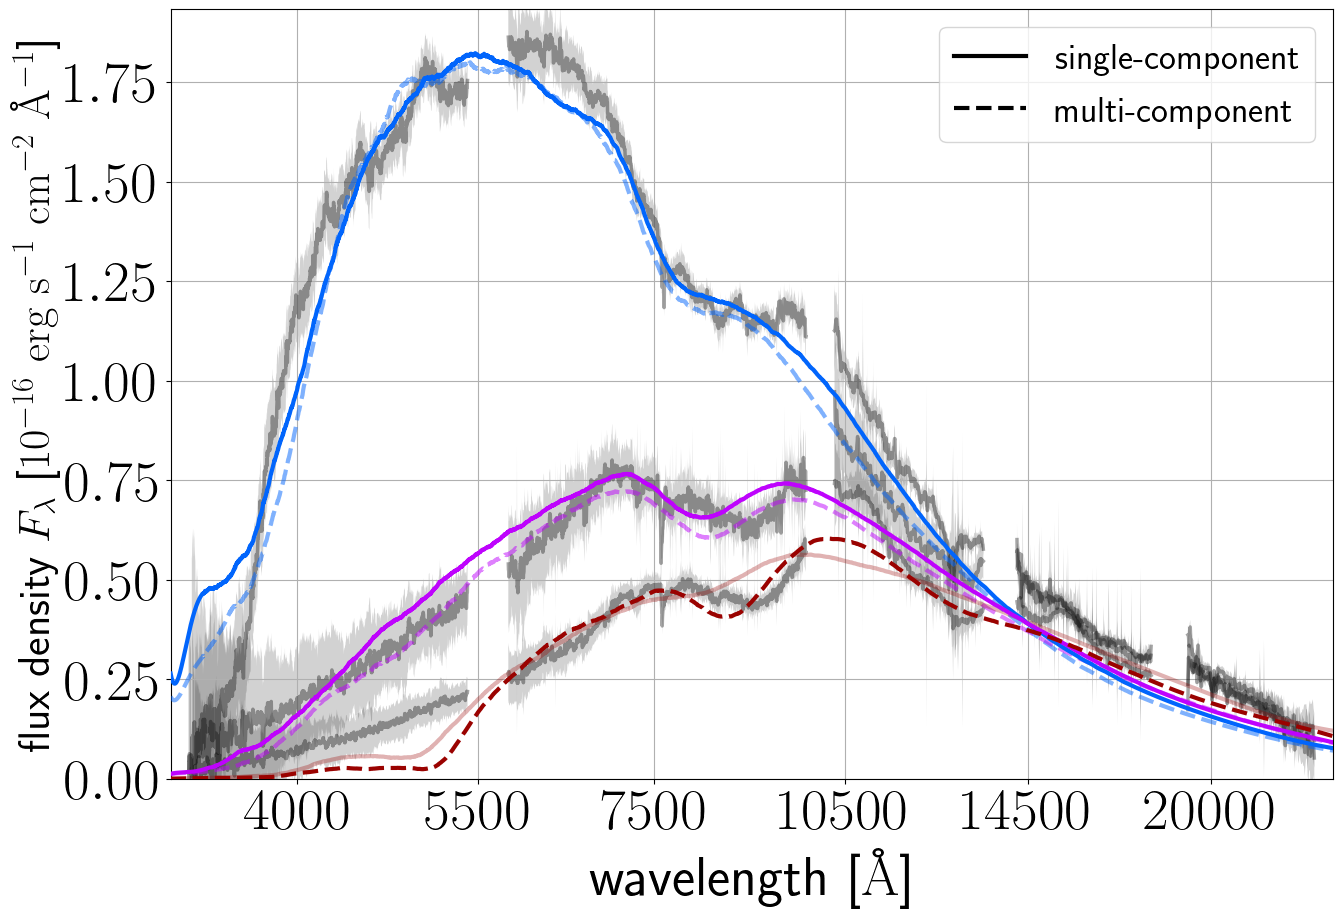
\includegraphics[width=0.98\textwidth]{figs/bestfits_compare_all_SPARK_2_highlighted.png}
    \figcaption{\textbf{Compilation of all best fit models to the spectrum of the GW170817 kilonova, AT2017gfo, from this work at 1.4, 2.4, and 3.4 days post-merger, for both single- and multi-component models.} The preferred models are highlighted; disfavored are more translucent. The single-component models are favored at 1.4 and 2.4 days (solid blue and purple lines). At 3.4 days, we require a multi-component ejecta to adequately fit the spectrum (dashed red line). The abundance patterns corresponding to these preferred models are included in Figure~\ref{fig:abunds_time_evolution}. Zoomed in versions of these best fits are included in Figures~\ref{fig:all_spec_single}~and~\ref{fig:all_spec_multi} (Appendix~\ref{app:allspec_posteriors}). Best fits are obtained as the median of the posterior, or the median of some mode of the posterior; these full posteriors are also included in Appendix~\ref{app:allspec_posteriors}.}\label{fig:bestfits}
\end{figure*}



%% best fit single-component parameters; Table 3
\begin{deluxetable}{cccc}
\centering
\tablecaption{Best fit parameters for single-component fits to the GW170817 kilonova at $1.4$, $2.4$, and $3.4$~days. The $1.4$~day fit is the ``purple + warm'' model of V23. $v_{\mathrm{outer}}$ is fixed to $0.35c$ in the 1.4 day fit. The inner boundary temperature $T_{\mathrm{inner}}$ and lanthanide mass fraction $X_{\mathrm{lan}}$ are derived parameters, \ie, they are not dimensions in $\theta$-space.}
\tablehead{parameter & 1.4 days & 2.4 days & 3.4 days}
\startdata\tablewidth{1.0\textwidth}
 \vspace{2pt}
$\log_{10}(\frac{L_\mathrm{outer}}{L_{\odot}})$ & $7.782^{+0.013}_{-0.014}$ & $7.594^{+0.040}_{-0.061}$ & $7.531^{+0.017}_{-0.016}$ \\ 
$\log_{10}(\frac{\rho_0}{\mathrm{g~cm^{-3}}})$ & $-15.016^{+0.320}_{-0.316}$ & $-15.443^{+0.742}_{-0.463}$ & $-14.586^{+0.313}_{-0.384}$ \\ 
$v_{\mathrm{inner}}/c$ & $0.313^{+0.013}_{-0.014}$ & $0.249^{+0.017}_{-0.032}$ & $0.253^{+0.011}_{-0.021}$ \\
$v_{\mathrm{outer}}/c$ & $0.35$ & $0.342^{+0.047}_{-0.050}$  & $0.309^{+0.032}_{-0.023}$ \\
$v_{\mathrm{exp}}/c$ & $0.240^{+0.055}_{-0.082}$ & $0.172^{+0.107}_{-0.101}$ & $0.132^{+0.094}_{-0.056}$ \\
$Y_e$ & $0.311^{+0.013}_{-0.011}$ & $0.306^{+0.055}_{-0.204}$ & $0.226^{+0.062}_{-0.067}$ \\
$s~[k_{\mathrm{B}}/\mathrm{nuc}]$ & $13.6^{+4.1}_{-3.0}$ & $17.6^{+7.1}_{-6.3}$ & $15.4^{+7.1}_{-6.3}$ \\ \hline
$T_{\mathrm{inner}}~[\mathrm{K}]$ & $3958^{+87}_{-94}$ & $3050^{+126}_{-223}$ & $2455^{+59}_{-104}$ \\ 
%$X_{\mathrm{lan}}$ & $1.8^{+26.3}_{-1.8}\times 10^{-7}$ & $9.5^{+355.1}_{-6.6}\times 10^{-8} $ & $\sim1.1\times 10^{-2}$\\
$\log_{10} X_{\mathrm{lan}}$ & ${-7.03}^{+0.46}_{-0.47}$ & $-5.64^{+1.05}_{-1.31}$ & $-2.10^{+1.28}_{-6.20}$ \\
\enddata
\end{deluxetable}\label{tab:bestfit_single}



%% best fit multi-component parameters; Table 4
\begin{deluxetable*}{cccc}
\centering
\tablecaption{Best fit parameters for multi-component fits to the GW170817 kilonova at $1.4$, $2.4$, and $3.4$~days. The ejecta mass in each component $M_{\mathrm{1; 2}}$, lanthanide mass fraction in each component $X_{\mathrm{lan,1; 2}}$, and the total $X_{\mathrm{lan,total}}$ are derived parameters.}
\tablehead{parameter & 1.4 days & 2.4 days & 3.4 days}
\startdata\tablewidth{1.0\textwidth}
 \vspace{2pt}
$\log_{10}(\frac{L_\mathrm{outer}}{L_{\odot}})$ & $7.854^{+0.012}_{-0.017}$ & $7.700^{+0.065}_{-0.073}$ & $7.605^{+0.049}_{-0.040}$ \\ 
$\log_{10}(\frac{\rho_0}{\mathrm{g~cm^{-3}}})$ & $-15.095^{+0.127}_{-0.401}$ & $-15.440^{+0.813}_{-0.467}$ & $-14.505^{+0.323}_{-0.372}$ \\ \hline
$v_{\mathrm{inner,1}}/c$ & $0.323^{+0.007}_{-0.020}$ & $0.260^{+0.061}_{-0.039}$ & $0.213^{+0.056}_{-0.035}$ \\
$v_{\mathrm{outer,1}}/c$ & $0.326^{+0.009}_{-0.012}$ & $0.335^{+0.054}_{-0.065}$ & $0.344^{+0.035}_{-0.038}$ \\
$v_{\mathrm{exp,1}}/c$ & $0.118^{+0.029}_{-0.025}$ & $0.170^{+0.108}_{-0.100}$ & $0.198^{+0.092}_{-0.102}$ \\
$Y_{e,1}$ & $0.139^{+0.028}_{-0.114}$ & $0.288^{+0.129}_{-0.187}$ & $0.228^{+0.073}_{-0.088}$ \\
$s_{1}~[k_{\mathrm{B}}/\mathrm{nuc}]$ & $24.6^{+3.4}_{-5.1}$ & $21.1^{+10.5}_{-9.5}$ & $14.9^{+8.0}_{-4.5}$ \\ \hline
$v_{\mathrm{inner,2}}/c$ & $0.281^{+0.011}_{-0.013}$ & $0.268^{+0.049}_{-0.045}$ & $0.232^{+0.038}_{-0.027}$ \\
$v_{\mathrm{outer,2}}/c$ & $0.355^{+0.015}_{-0.015}$ & $0.335^{+0.045}_{-0.070}$ & $0.334^{+0.037}_{-0.022}$ \\
$v_{\mathrm{exp,2}}/c$ & $0.195^{+0.034}_{-0.036}$ & $0.183^{+0.089}_{-0.110}$ & $0.134^{+0.091}_{-0.069}$ \\
$Y_{e,2}$ & $0.340^{+0.022}_{-0.021}$ & $0.261^{+0.163}_{-0.124}$ & $0.161^{+0.149}_{-0.104}$ \\
$s_{2}~[k_{\mathrm{B}}/\mathrm{nuc}]$ & $20.1^{+3.8}_{-3.6}$ & $22.0^{+10.0}_{-10.1}$ & $21.5^{+8.3}_{-9.5}$ \\ \hline\hline
$M_{1}~[M_{\odot}]$ & $6.9^{+22.1}_{-6.0} \times 10^{-7}$ & $2.3^{+12.5}_{-0.7}\times 10^{-5}$ & $5.3^{+1.8}_{-1.3}~\times 10^{-4}$ \\
%$X_{\mathrm{lan,1}}$ & & $\sim1.1\times10^{-5}$ & $\geqslant 1.67 \times 10^{-2}$ \\ \hline
$\log_{10} X_{\mathrm{lan,1}}$ & $-1.08^{+0.34}_{-0.34}$ & $-0.63^{+0.26}_{-11.1}$ & $-0.97^{+0.23}_{-0.32}$ \\ \hline
$M_{2}~[M_{\odot}]$ & $7.0^{+0.8}_{-1.0} \times 10^{-5}$ & $4.0^{+4.8}_{-0.9}\times 10^{-5}$ & $3.8^{+1.1}_{-0.9}~\times 10^{-4}$ \\
% $X_{\mathrm{lan,2}}$ & & $\sim2.4\times10^{-3}$ & $2.8^{+26.3}_{-1.1}\times10^{-2}$ \\ \hline
$\log_{10} X_{\mathrm{lan,2}}$ & ${-12.99}^{+3.15}_{-3.45}$ & $-4.53^{+2.61}_{-3.53}$ & $-0.88^{+0.32}_{-0.55}$ \\ \hline
$\log_{10} X_{\mathrm{lan,total}}$ & $-12.99^{+8.82}_{-3.45}$ & $-3.39^{+1.34}_{-1.75}$ & $-0.97^{+0.23}_{-0.32}$ \\
\enddata
\end{deluxetable*}\label{tab:bestfit_multi}


%% abundance patterns; Fig. 2
\begin{figure*}[!ht]
    \centering
    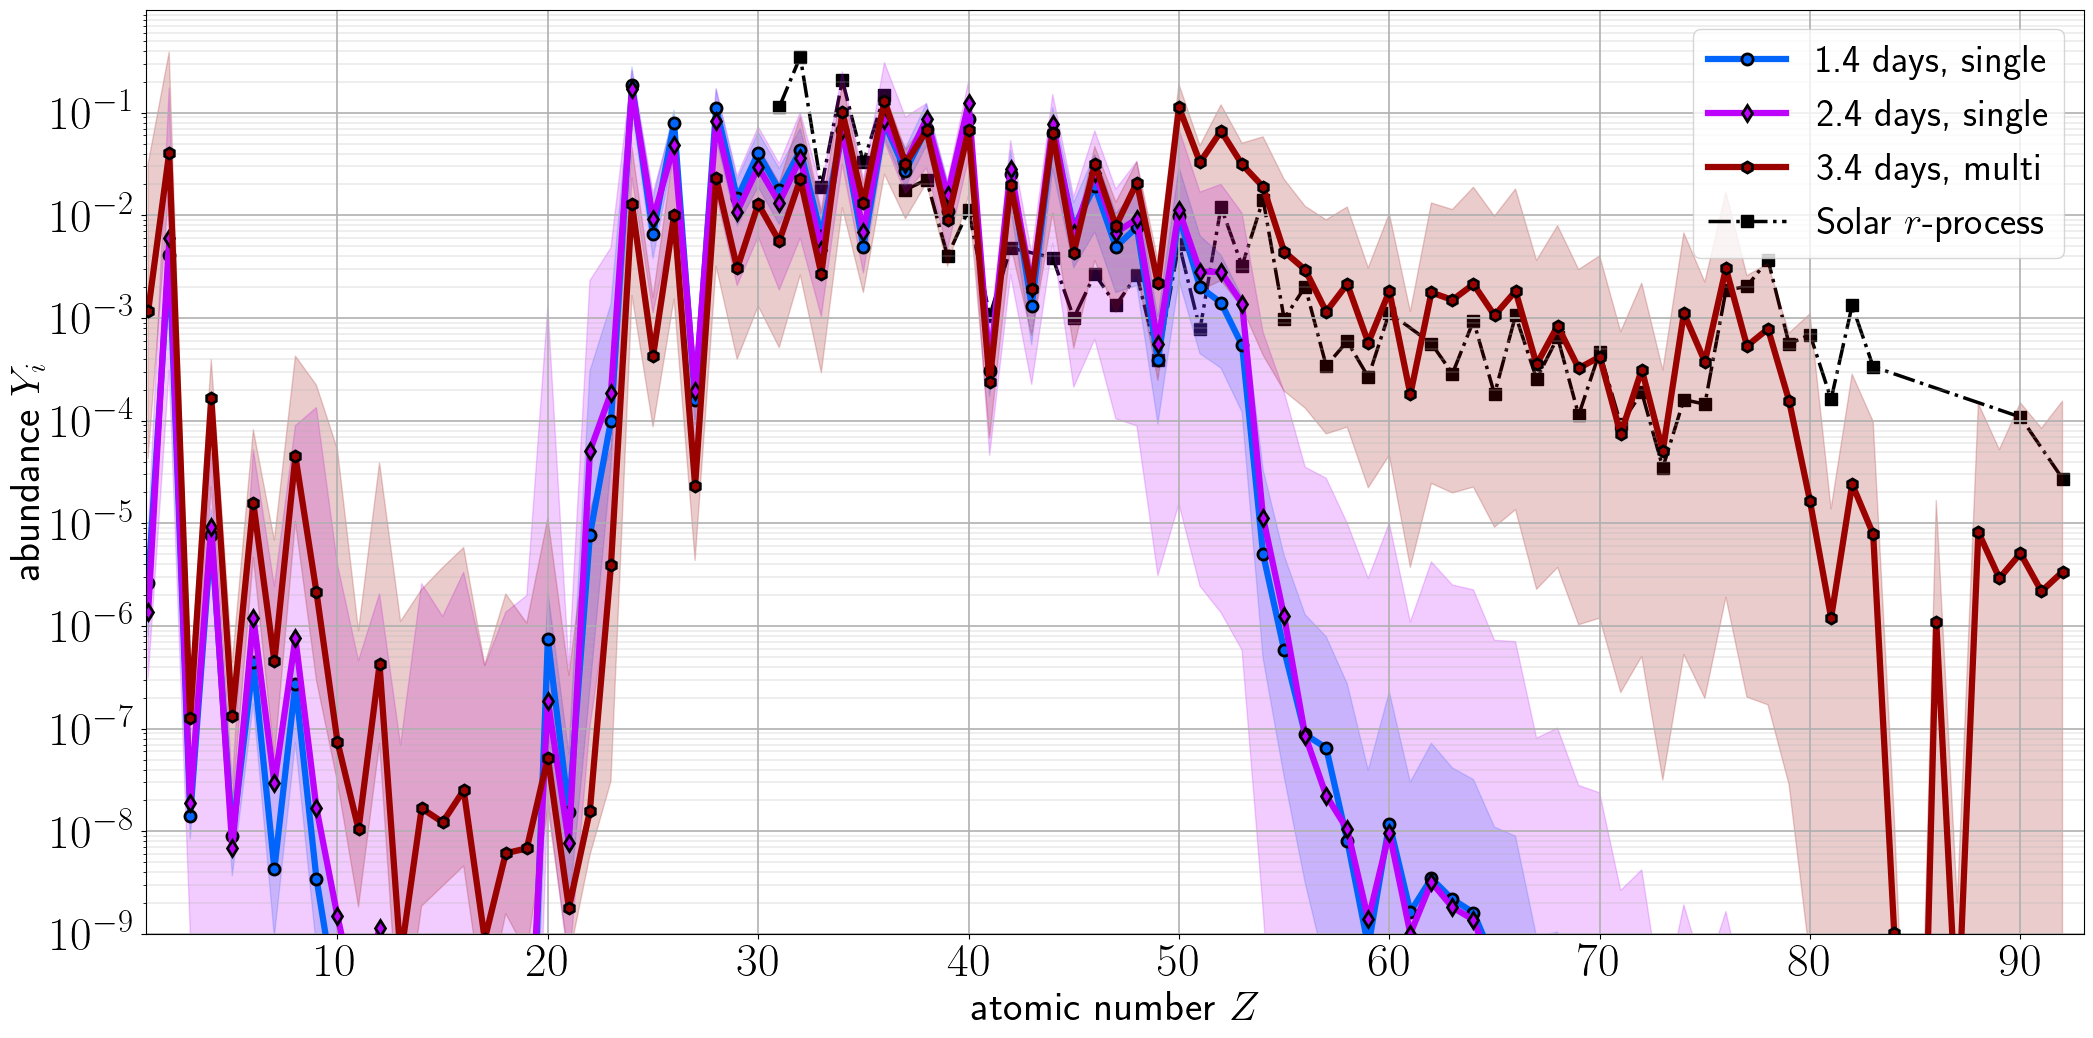
\includegraphics[width=0.98\textwidth]{figs/compare_abunds_220808_014638-221022_084052-230622_230103_posterior_100samples_dynesty.png}
    \figcaption{\textbf{Best fit abundance patterns at 1.4, 2.4, and 3.4 days.} The abundances at 1.4 and 2.4 days are taken from the preferred single-component fits, while the abundance at 3.4 days is taken from the preferred multi-component fit (see Figure~\ref{fig:bestfits}). The overall abundance of the multi-component ejecta at 3.4 days is the mass-weighted sum over all 10 shells in the stratified ejecta. A new, redder kilonova component emerges at 3.4 days post-merger. Uncertainty bands are obtained by taking additional samples from the the posterior, effectively propagating the uncertainty on $Y_e$, $v_{\mathrm{exp}}$, and $s$ into the abundances. We also show the Solar $r$-process pattern, computed using data from \cite{lodders09} subtracted by the $s$-process residuals of \cite{bisterzo14}. The best fit abundances are evidently non-Solar at the first two epochs, but are closer to Solar at the third.}\label{fig:abunds_time_evolution}
\end{figure*}


%% wedges; Fig 3
\begin{figure}[!ht]
    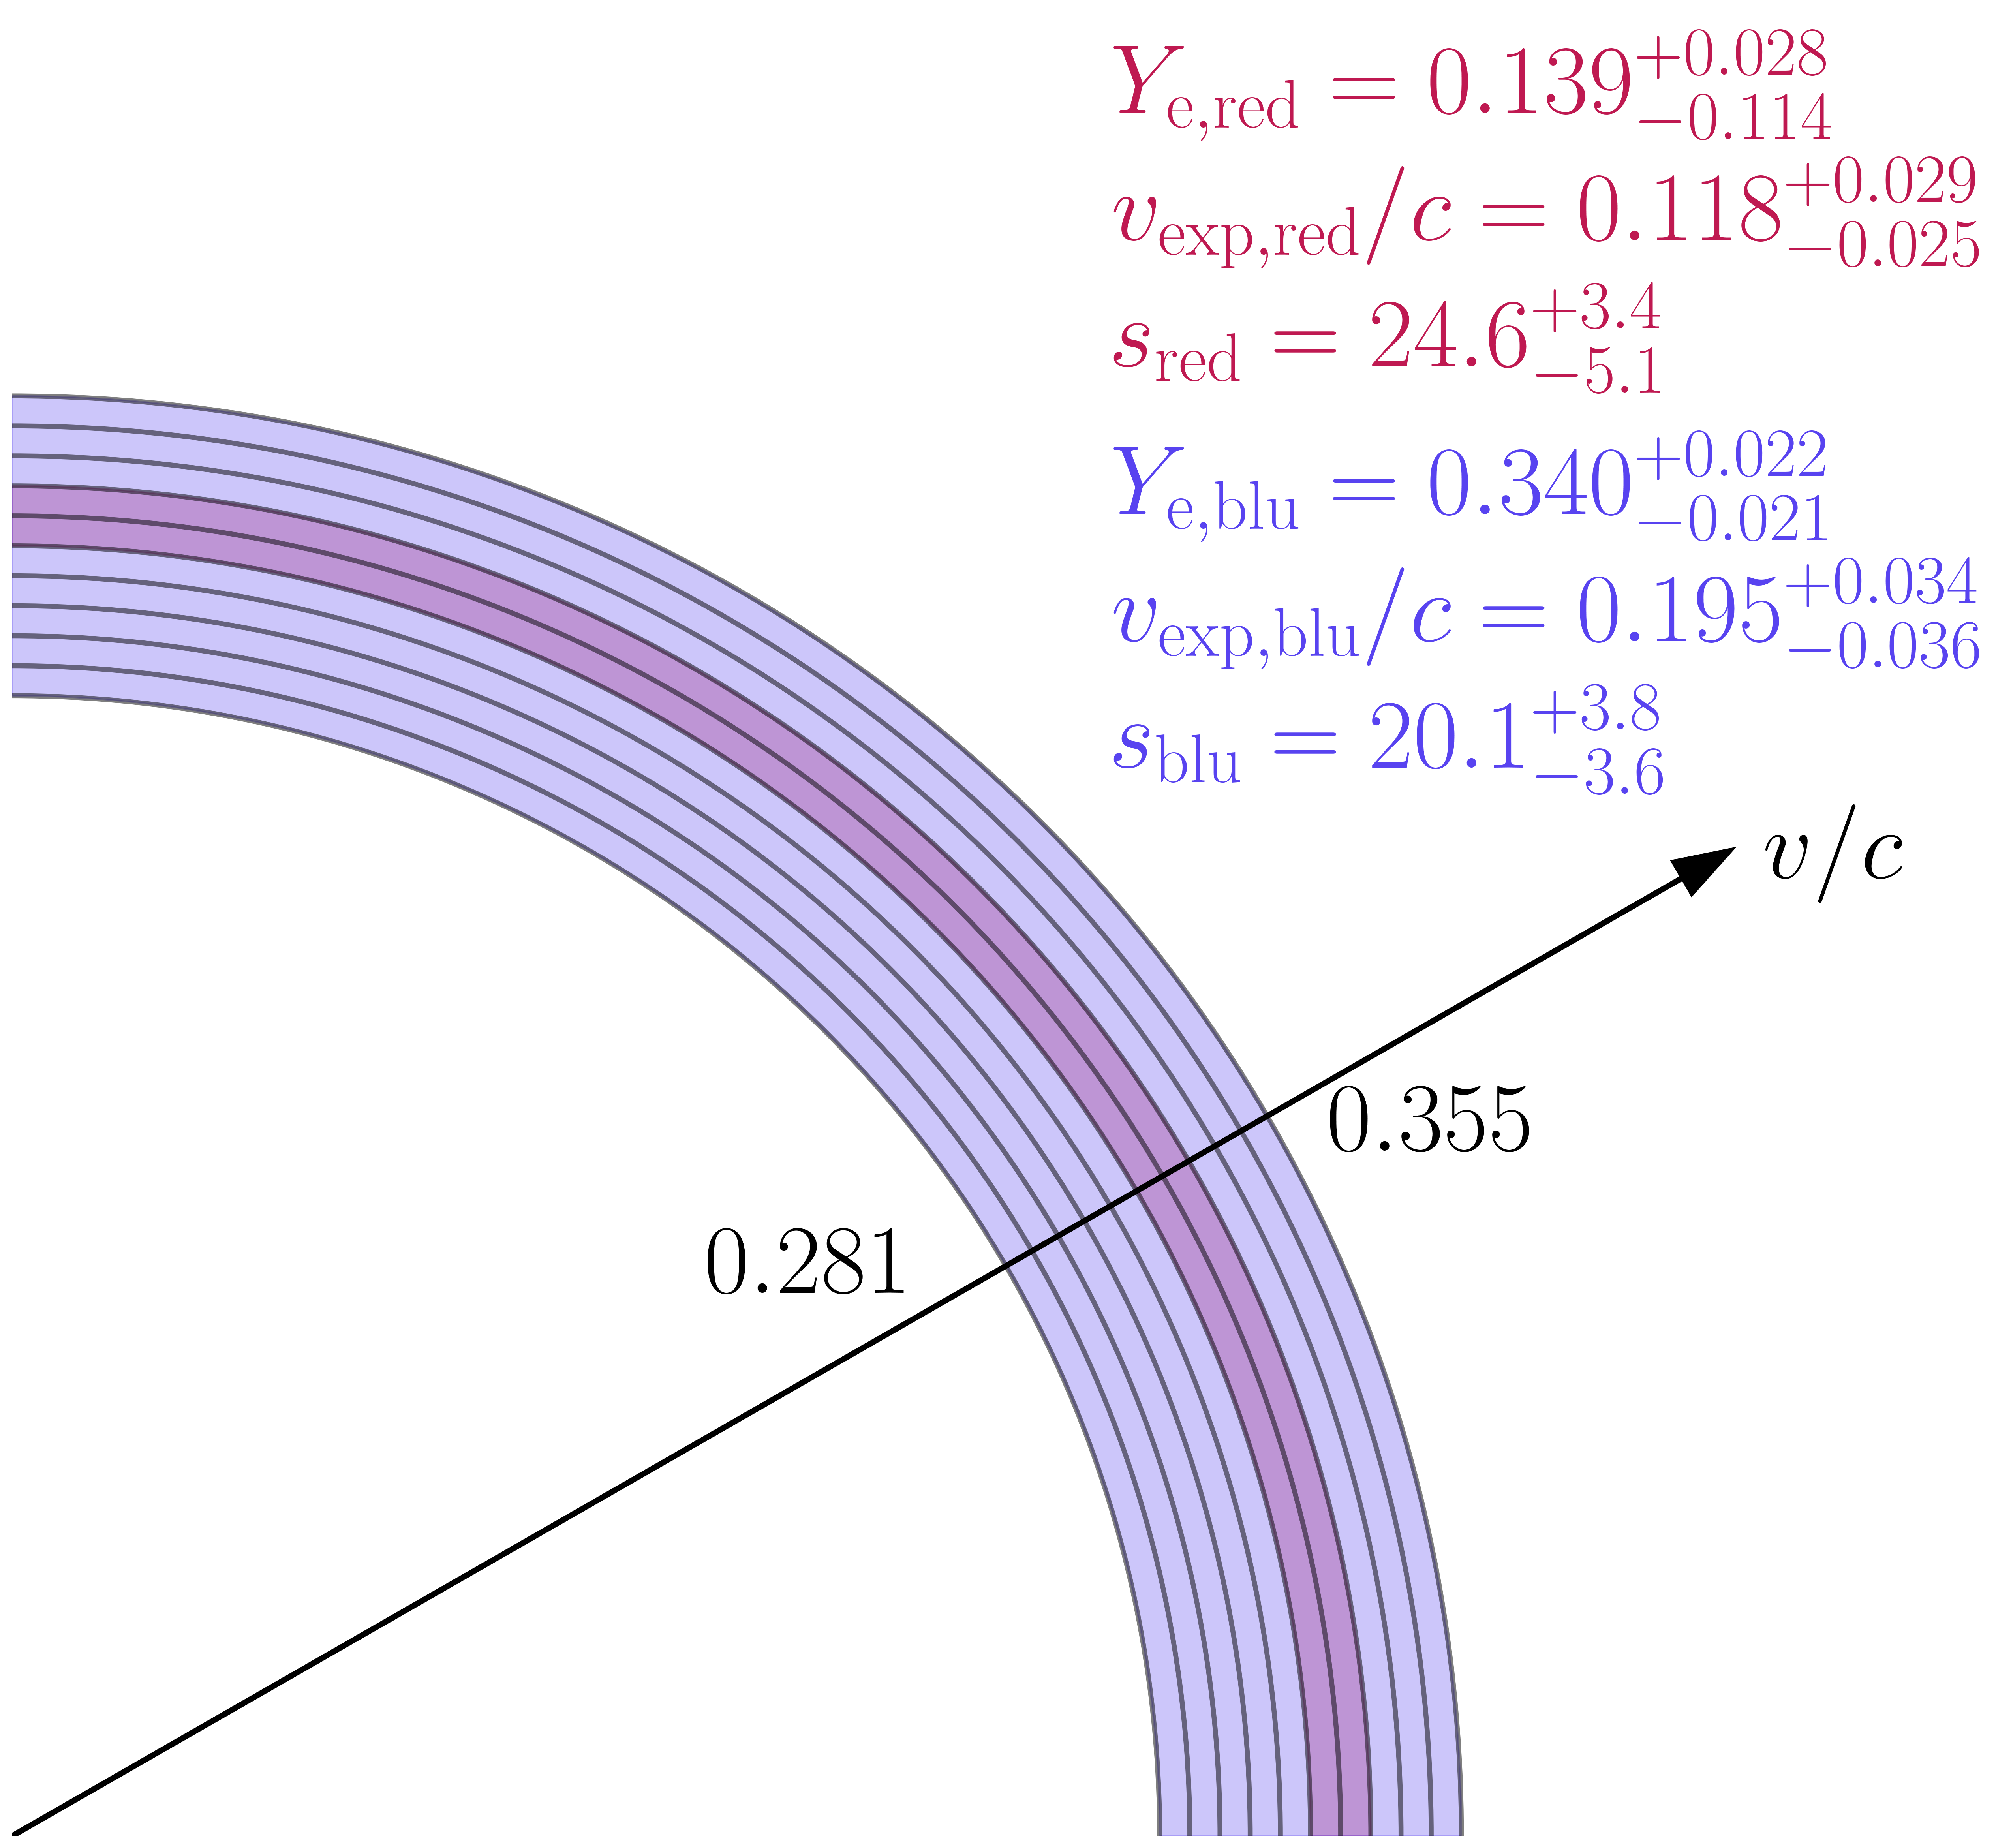
\includegraphics[width=0.35\textwidth]{figs/multicomp_wedges_1.4d.png}
    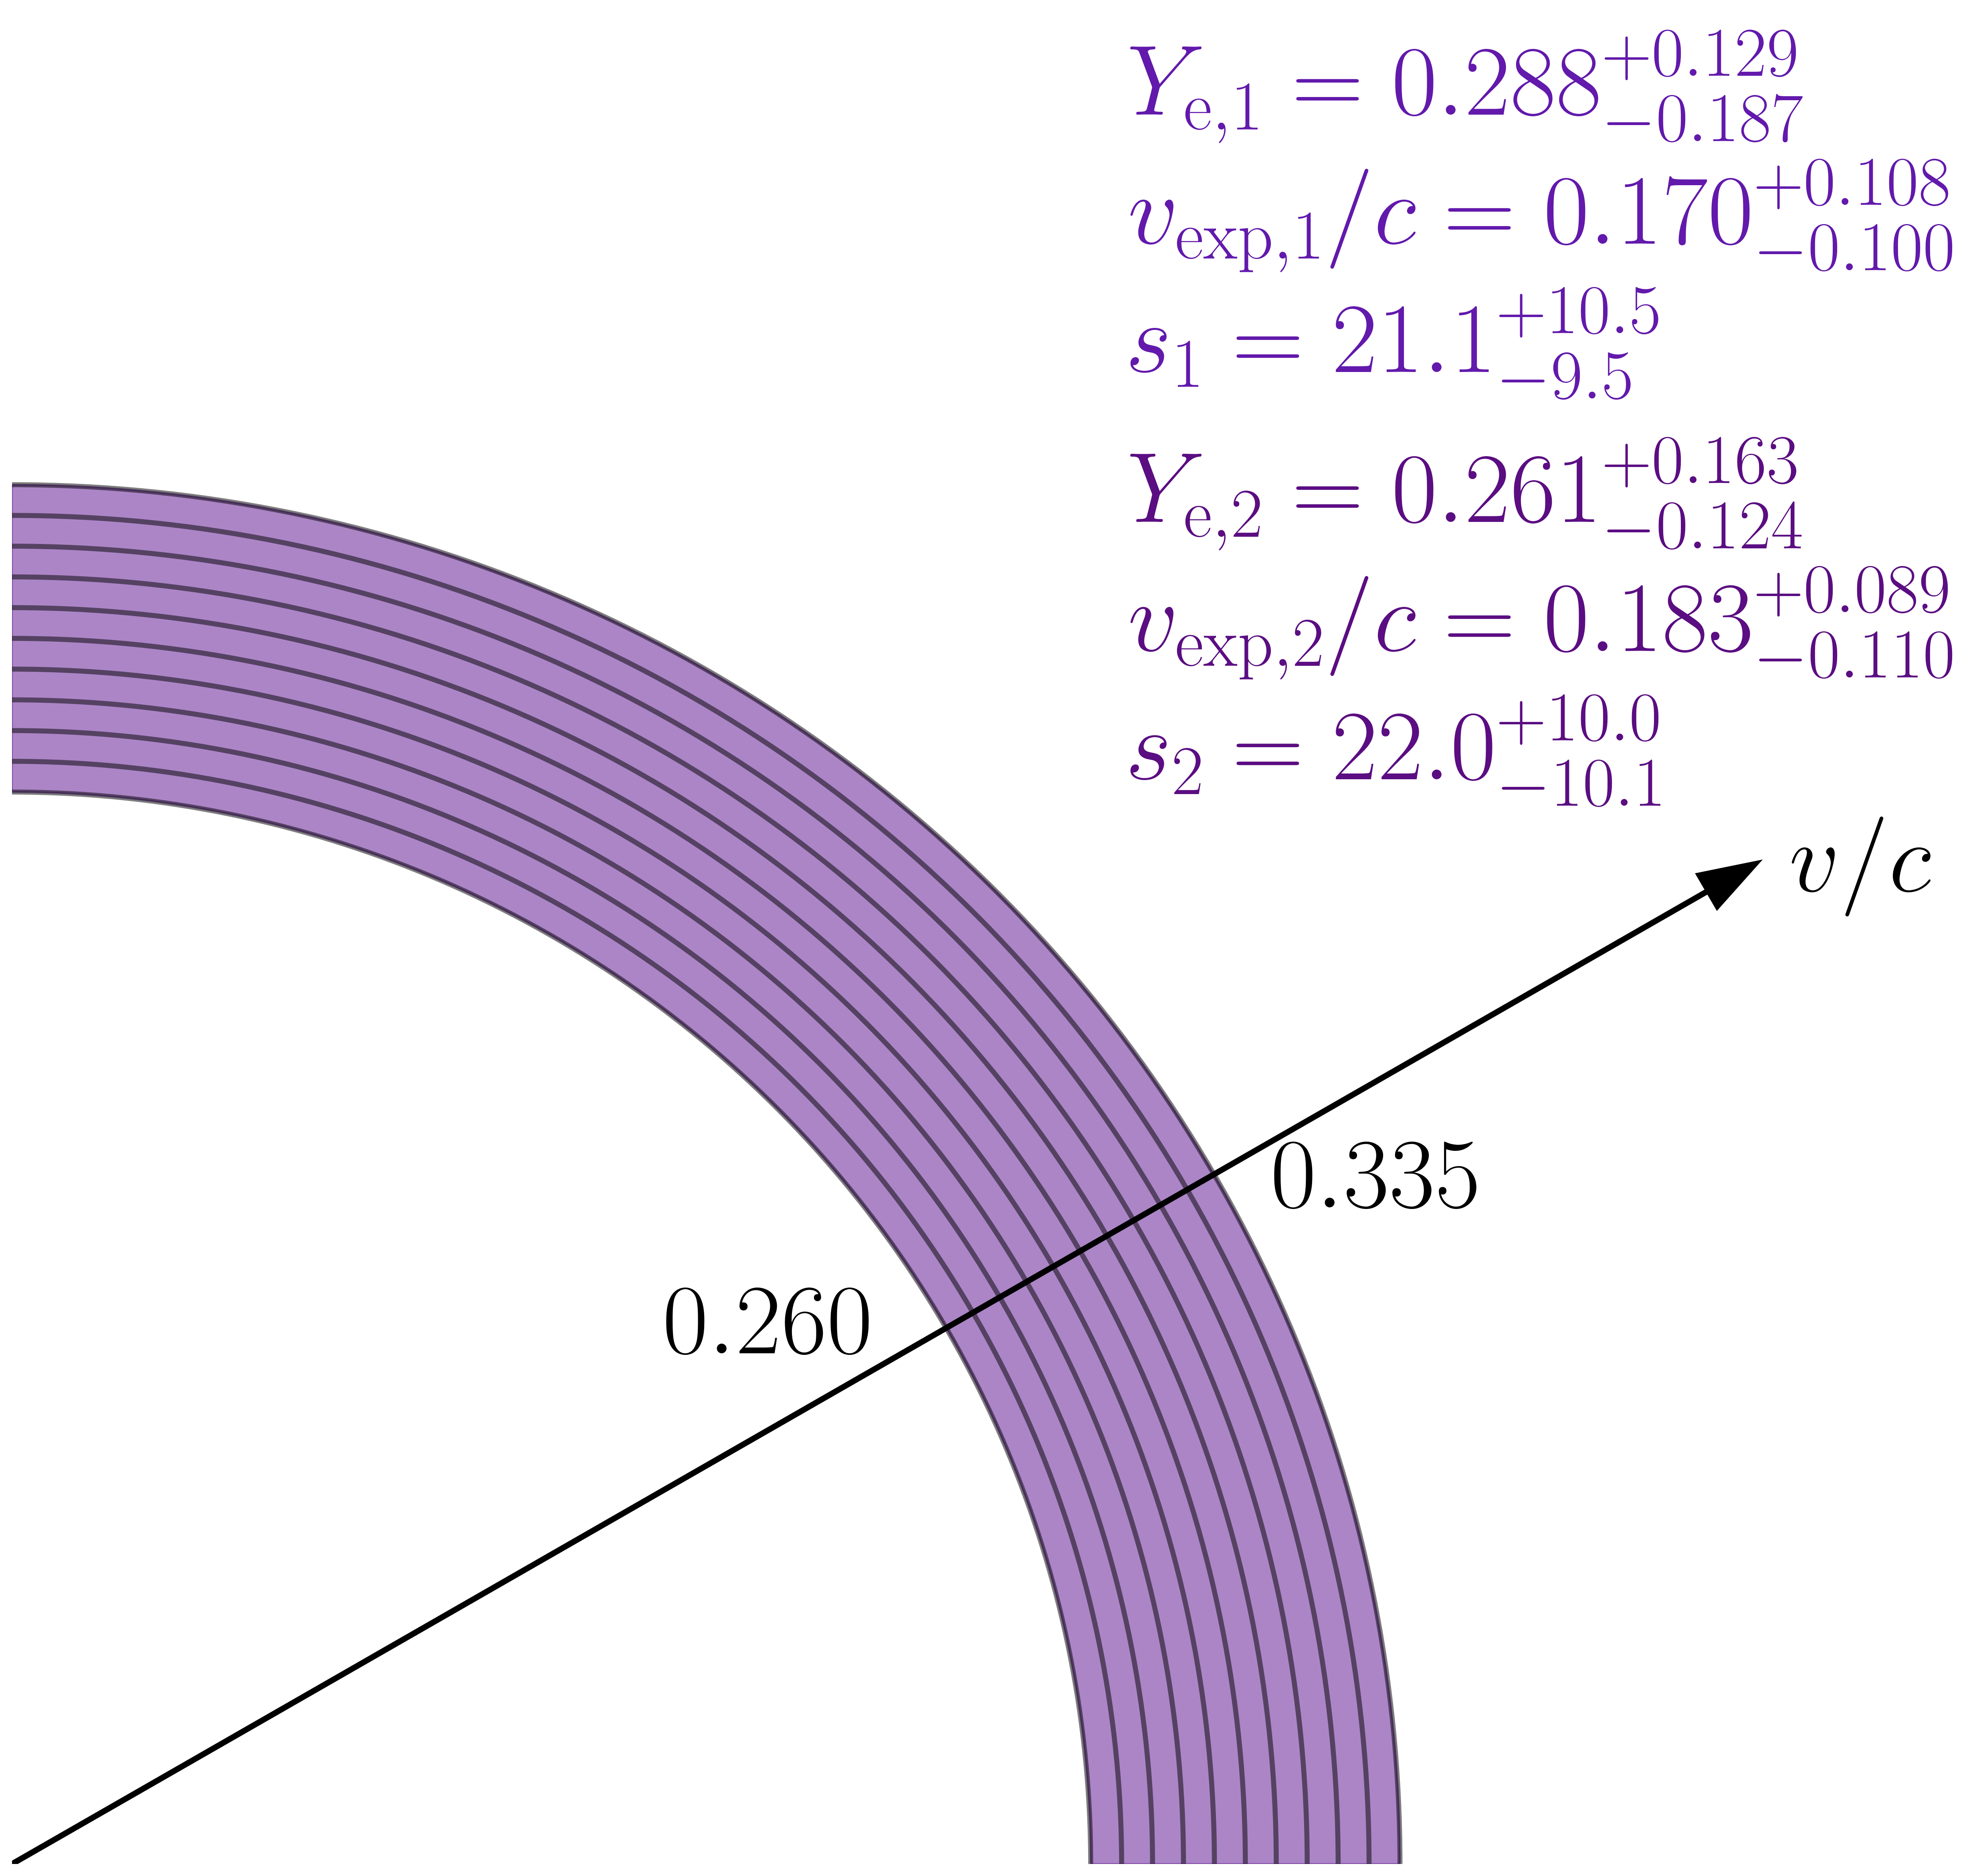
\includegraphics[width=0.35\textwidth]{figs/multicomp_wedges_2.4d.png}
    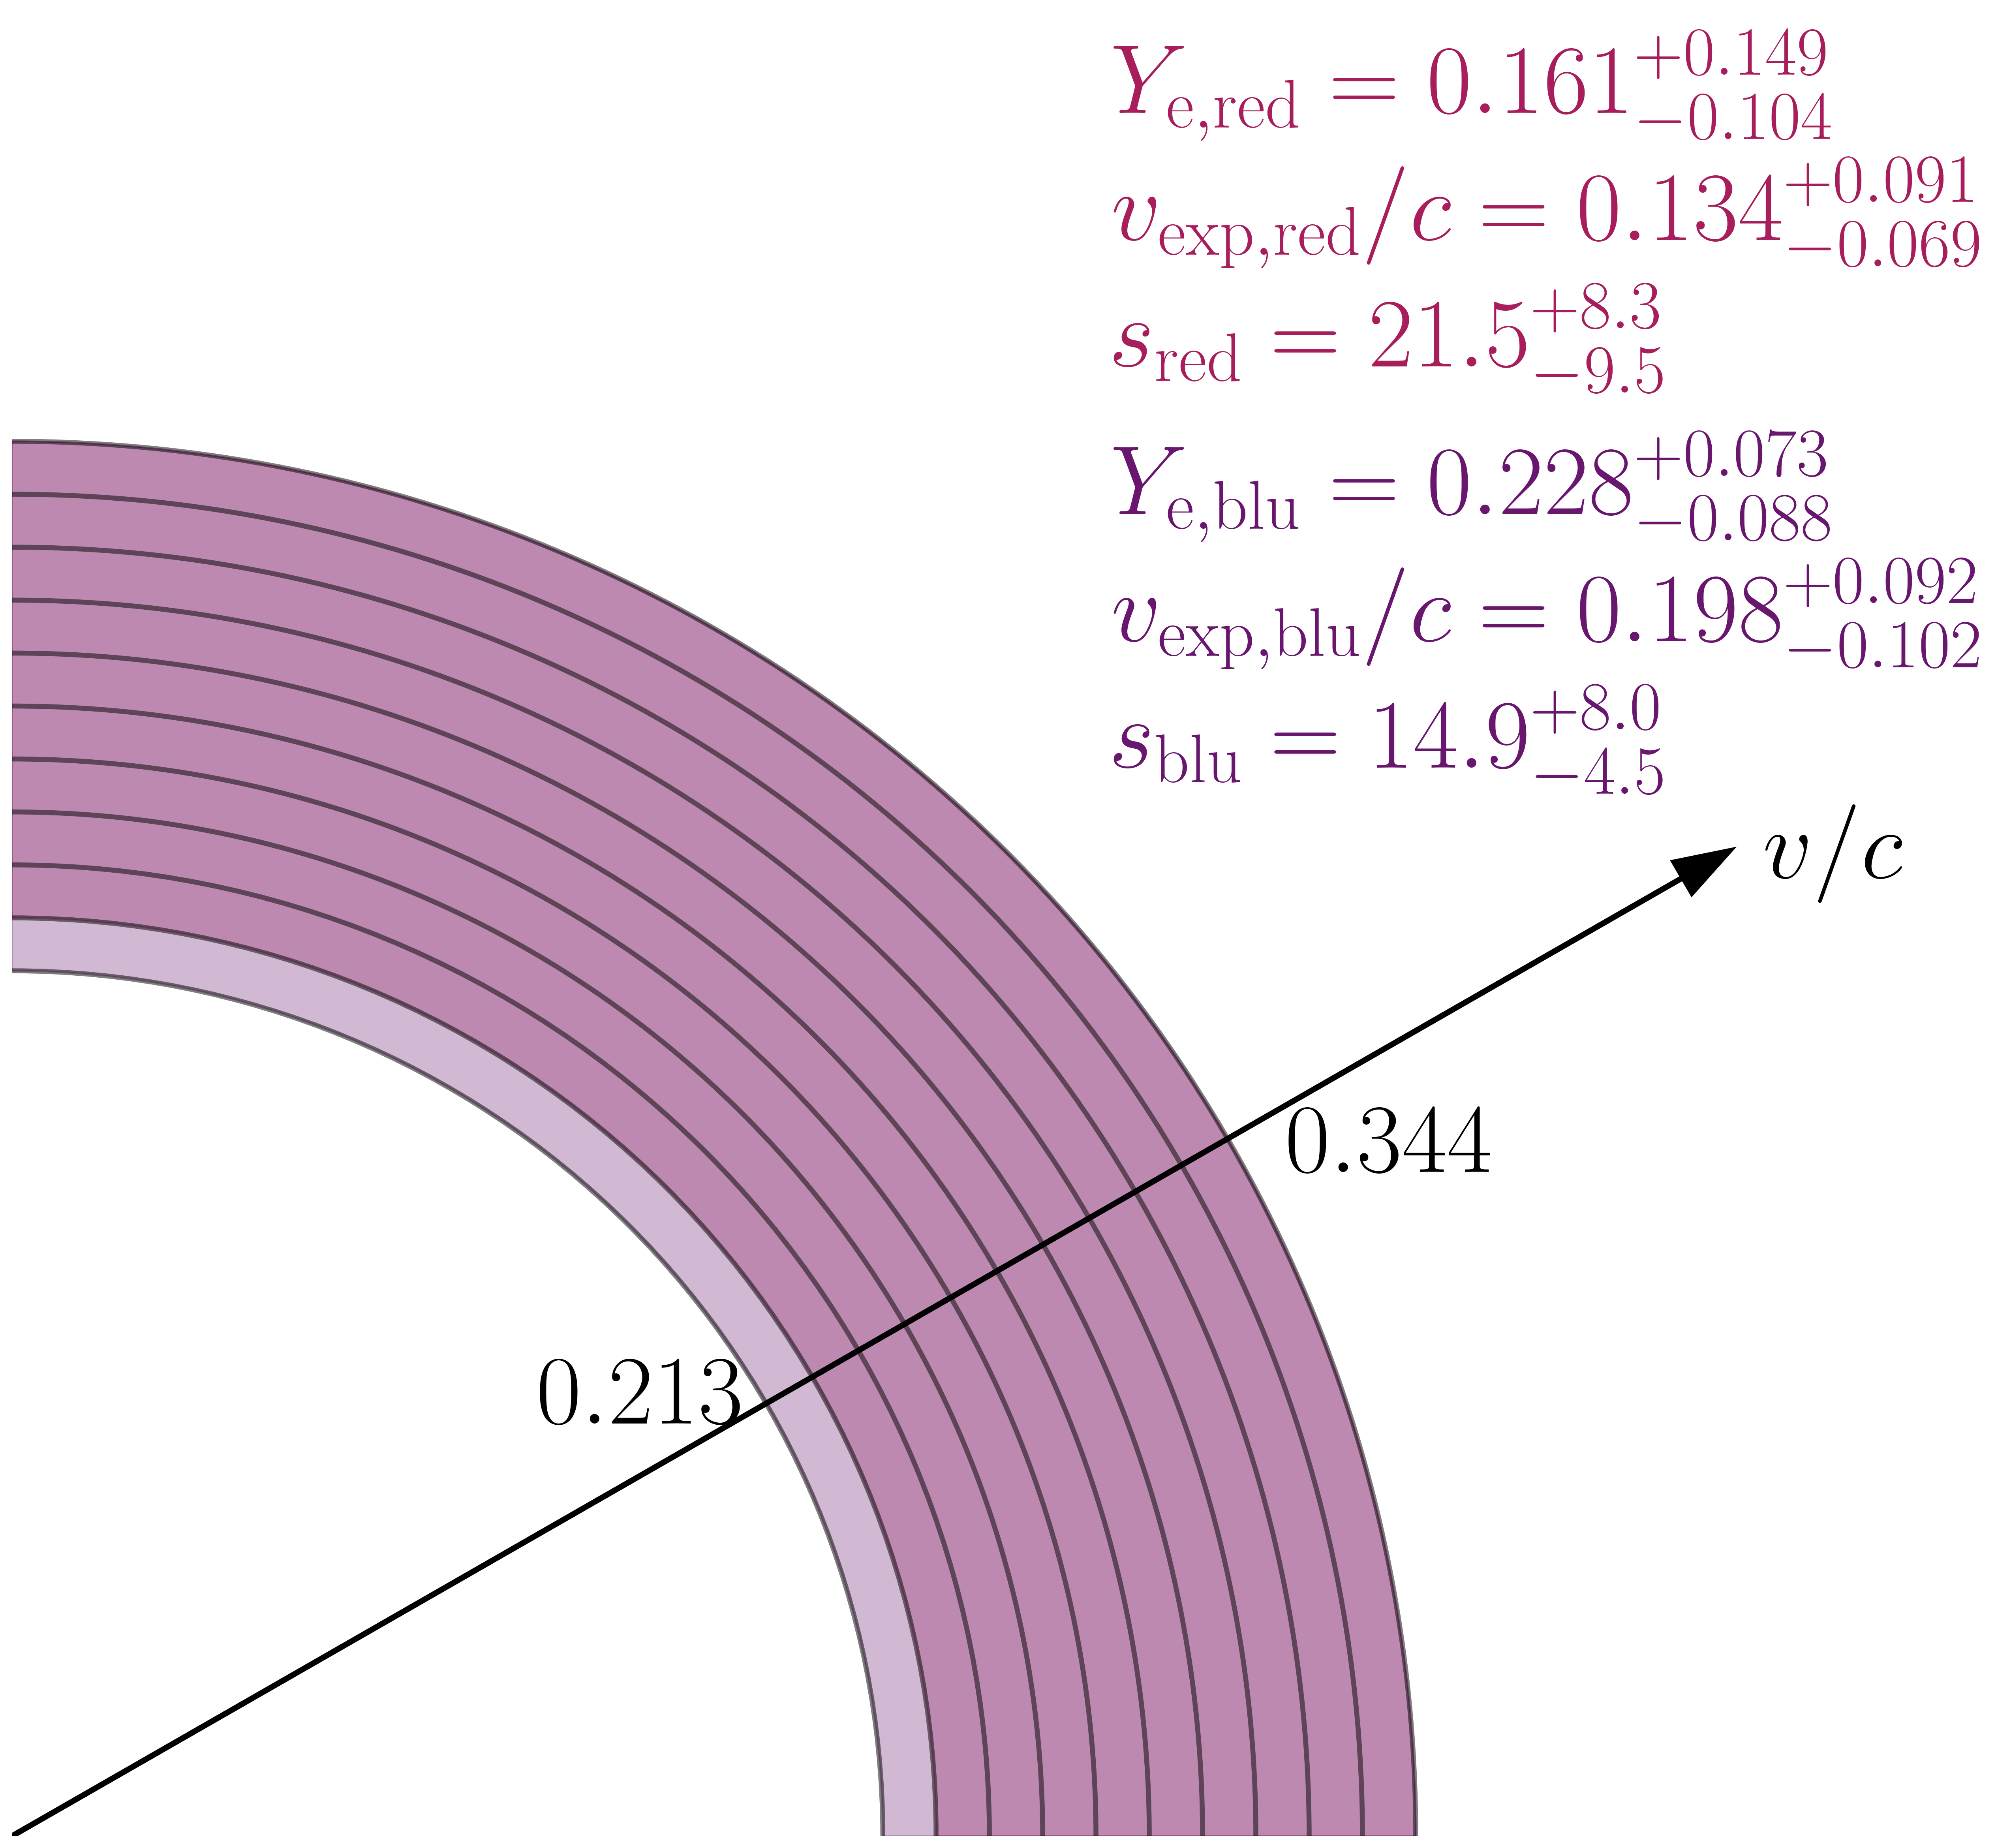
\includegraphics[width=0.35\textwidth]{figs/multicomp_wedges_3.4d.png}
    \figcaption{\textbf{Inferred ejecta configuration and composition-setting parameters for the multi-component fits.} Best fits are taken as the median of the posteriors, included in Appendix~\ref{app:allspec_posteriors}. The abundance patterns of each component are compared in Appendix~\ref{app:compare_components}. \textit{Top to bottom:} 1.4, 2.4, and 3.4 days. At 1.4 days, a thin ``red'' component which contains $\sim1$\% of the total ejecta mass is seen. This component has a negligible impact on the emergent spectrum, indicating that this model is effectively single-component. At 2.4 days, two components with remarkably similar compositions completely overlap in space, also effectively indicating a single-component ejecta. At 3.4 days, two components with different compositions are present; the ejecta is multi-component. }\label{fig:infer_multicomp_wedges}
\end{figure}





We model the 1.4, 2.4, and 3.4 day spectra of AT2017gfo with single- and multi-component (2-component) models, and compare the models at each epoch. In Figure~\ref{fig:bestfits}, we compile our best fit spectra, and highlight our favored models. The parameters for our best fit single- and multi-component models are included in Tables~\ref{tab:bestfit_single}~and~\ref{tab:bestfit_multi}, respectively. We find that a single-component blue ejecta model best describes the 1.4 and 2.4 day spectra, while at 3.4 days, we require an additional red, lanthanide-rich component in a multi-component ejecta configuration. In the following sections, we present and examine each of the best fits in turn, at each epoch. 

Appendix~\ref{app:allspec_posteriors} contains compilations of all $m_0 + m_{\mathrm{active}}$ spectra generated in a given \SPARK~run, for the 1.4, 2.4, and 3.4 day single- and multi-component runs. Posteriors generated by the single- and multi-component runs are also included. Unless stated otherwise, we use the median and 2.5\% / 97.5\% quantiles of the posterior, or the median and these quantiles of some mode of a multi-modal posterior, to determine our best fit and uncertainties. The convergence of the posteriors is assessed in Appendix~\ref{app:convergence}.



%%% subsection 3.1: 1.4 DAYS
\subsection{Single-and multi-component modelling at 1.4 days}\label{ssc:1.4}

In V23, we fit the 1.4 day spectrum of AT2017gfo with a single-component ejecta model. This fit required $m_0 + m_{\mathrm{active}} = 1500 + 1140$ points to obtain a good fit and converged posterior (see Figure~\ref{fig:all_spec_single}). We describe the best fit ``purple + warm'' model here, and refer the reader to V23 for greater details. The purple + warm model is characterized by a photospheric velocity of $v_{\mathrm{inner}}/c = 0.313^{+0.013}_{-0.014}$; while the outer boundary velocity was fixed to $v_{\mathrm{outer}} = 0.35c$. For abundance-setting parameters, we find an electron fraction $Y_e = 0.311^{+0.013}_{-0.011}$, expansion velocity of $v_{\mathrm{exp}}/c = 0.240^{+0.055}_{-0.082}$, and entropy of $s / k_{\mathrm{B}} = 13.6^{+4.1}_{-3.0}$. In V23, we referred to this model as ``purple + warm'', but emphasize that this is nonetheless substantially blue ejecta within the broader context of kilonova components. These parameters point to an abundance pattern which is poor in lanthanides, but rich in strontium (${}_{38}$Sr), allowing for a good fit to the prominent $\sim$8000~\AA~feature. The fit struggles at shorter wavelengths: over $3500-4500$~\AA, we overestimate the absorption from yttrium (${}_{39}$Y) and zirconium (${}_{40}$Zr), while at $\lesssim$3500~\AA, we underestimate. Nonetheless, the single-component model remains our preferred model at 1.4 days, as we elaborate on below.

We require $m_0 + m_{\mathrm{active}} = 1500 + 1440$ points to obtain a good fit and converged posterior in our 1.4 day, multi-component \SPARK~run (see Figure~\ref{fig:all_spec_multi}). Due to the increased dimensionality of the multi-component fits, more active learning samples are required than for single-component. The resultant fit generally captures the shape of the spectrum, and the broad absorption at $\sim$8000~\AA, like the single-component equivalent. However, the fit does not capture the continuum at wavelengths $\gtrsim$10,500 \AA~nor wavelengths in the range $\sim$3500 - 5000~\AA. The fit is marginally closer to the observed spectrum at the shortest wavelengths ($\lesssim$ 3500 \AA) but this region lies at the edge of the X-shooter spectrograph's sensitivity, and overall the single-component model is favored by visual inspection. 

We infer an outer boundary luminosity of $\log_{10} (L_{\mathrm{outer}}/L_{\odot}) = 7.854^{+0.012}_{-0.017}$, or equivalently, $L_{\mathrm{outer}} = 2.74^{+0.03}_{-0.02}~\times 10^{41}~\mathrm{erg~s^{-1}}$. This is brighter than is inferred in the single-component equivalent. This is as expected: due to the use of 30 \TARDIS~iterations (rather than 1), $L_{\mathrm{outer}}$ is updated at each iteration. Hence, in our multi-component models, the meaning of $L_{\mathrm{outer}}$ is different and cannot be mapped directly to $T_{\mathrm{inner}}$. ($L_{\mathrm{outer}}$ is also higher in the 2.4 and 3.4 day multi-component models, compared to the single-component equivalents).

We infer two components with different abundance-setting parameters, but find that one of these components dominates over the other. This first component is described by a low electron fraction $Y_{e,1} = 0.139^{+0.028}_{-0.114}$ and specific entropy $s_1 / k_{\mathrm{B}} = 24.6^{+3.4}_{-5.1}$, and could thus be described as red. The latter has $Y_{e,2} = 0.340^{+0.022}_{-0.021}$ and $s_2 / k_{\mathrm{B}} = 20.1^{+3.8}_{-3.6}$, and is bluer. As in the single-component fits, expansion velocities ($v_{\mathrm{exp},1}$ and $v_{\mathrm{exp},2}$) are poorly constrained. The entropies ($s_1$ and $s_2$), although better constrained, are both higher than and inconsistent with the single-component equivalent at 1.4 days. The $Y_{e,2}$ of the second, bluer component is consistent with the purple + warm model.  

A physical picture for the components is included in Figure~\ref{fig:infer_multicomp_wedges}. We see that the red component is confined to only 2 shells, while the blue component extends over a greater radius. The mass contained in these two components is $M_1/M_{\odot} = 6.9^{+22.1}_{-6.0} \times 10^{-7}$ and $M_2/M_{\odot} = 7.0^{+0.8}_{-1.0} \times 10^{-5}$, respectively. The bluer component thus contains $\sim$100$\times$ as much mass as the redder, and dominates the absorption/emission in the spectrum. In this sense, despite the different compositions of the two components (Figure~\ref{fig:abunds_components_compare}, Appendix~\ref{app:compare_components}), we interpret this multi-component \SPARK~run as converging to an effectively single-component model.




%%% subsection 3.2: 2.4 DAYS
\subsection{Single-and multi-component modelling at 2.4 days}\label{ssc:2.4}

We require $m_0 + m_{\mathrm{active}} = 1500 + 600$ points to obtain a good fit and converged posterior in our 2.4 day, single-component \SPARK~run (see Figure~\ref{fig:all_spec_single}). The resultant posterior shows some bimodality, most evident in the $s/k_{\mathrm{B}}$ dimension. Discarding samples from the posterior with $s/k_{\mathrm{B}} \geqslant 25.0$, we obtain a superior fit, and use this as our preferred model. This fit captures most of the continuum of the observed spectrum, and most of the $\sim$8000 \AA~absorption. If this absorption belongs to a P Cygni feature (as has been argued in \citealt{watson19, sneppen23}), we partially miss the red wing of this feature. Furthermore, we overestimate the absorption, or underestimate the continuum, at wavelengths $\lesssim$4500 \AA. 

We infer an $\log_{10} (L_{\mathrm{outer}}/L_{\odot}) = 7.594^{+0.040}_{-0.061}$. In the case of single-shell, single-iteration \TARDIS~runs, we can use these values to determine an inner boundary temperature of $T_{\mathrm{inner}} = 3050^{+126}_{-223}~\mathrm{K}$. As expected, the kilonova has dimmed and cooled since the previous epoch. The inferred velocities also match expectations: we obtain inner and outer boundary velocities $v_{\mathrm{inner}}/c = 0.249^{+0.017}_{-0.032}$ and $v_{\mathrm{outer}} = 0.342^{+0.047}_{-0.050}$. This $v_{\mathrm{outer}}$ is consistent with the fixed $v_{\mathrm{outer}} = 0.35c$ from 1.4 days, while $v_{\mathrm{inner}}$ (effectively the photospheric velocity) has receded into the ejecta, compared to $0.31c$ at 1.4 days. This is evidence for the ejecta expanding, cooling, and become optically thinner, as expected.

Finally, we obtain $Y_e = 0.306^{+0.055}_{-0.204}$ and $s/k_{\mathrm{B}} = 17.6^{+7.1}_{-6.3}$. As at 1.4 days, $v_{\mathrm{exp}}$ is poorly constrained. $s$ is better-constrained, and is also consistent with the earlier epoch. The posterior distribution in all dimensions is wider at this epoch; in particular, $Y_e$ exhibits a tail extending to smaller electron fractions. The posterior is nonetheless peaked at $Y_e = 0.306^{+0.055}_{-0.204}$, which is slightly lower than at 1.4 days, but consistent within uncertainties. 

We require $m_0 + m_{\mathrm{active}} = 1500 + 1020$ points to obtain a good fit and converged posterior in our 2.4 day, multi-component \SPARK~run (see Figure~\ref{fig:all_spec_multi}). The resultant fit once again captures the broad shape and some of the $\sim$8000~\AA~absorption. However, the depth of the $\sim$8000~\AA~absorption feature is overestimated. The multi-component fit does achieve a better fit to the continuum, at wavelengths $\lesssim$7000~\AA. 

The posterior for the multi-component, 2.4 day run is broader than the other epochs, as is the case for the single-component equivalent. As expected, the inferred model is dimmer than at 1.4 days. The two inferred components are remarkably similar: the first component is described by $Y_{e,1} = 0.288^{+0.129}_{-0.187}$ and $s_1 / k_{\mathrm{B}} = 21.1^{+10.5}_{-9.5}$, while the latter has $Y_{e,2} = 0.261^{+0.163}_{-0.124}$ and $s_2 / k_{\mathrm{B}} = 22.0^{+10.0}_{-10.1}$. Again, expansion velocities are poorly constrained, while the better-constrained entropies are higher than and inconsistent with the single-component equivalent. However, both entropies are consistent with the entropies inferred in the 1.4 day, multi-component model. Finally, $Y_{e,1}$ and $Y_{e,2}$ are both lower than, but still consistent with, the dominant blue component in the 1.4 day, multi-component model and the 1.4 day, single-component model.

A physical picture for the components is included in Figure~\ref{fig:infer_multicomp_wedges}. As expected, the photosphere recedes into the ejecta. The two components almost completely overlap in physical space. Indeed, the mass contained in these two components is $M_1/M_{\odot} = 2.3^{+12.5}_{-0.7} \times 10^{-5}$ and $M_2/M_{\odot} = 4.0^{+4.8}_{-0.9} \times 10^{-5}$, respectively; the ejecta mass is nearly equally partitioned into these two components. Furthermore, the similarity between $(Y_{e,1},~v_{\mathrm{exp},1},~s_1)$ and $(Y_{e,2},~v_{\mathrm{exp},2},~s_2)$ yields extremely similar compositions for both components (see Figure~\ref{fig:abunds_components_compare} in Appendix~\ref{app:compare_components}). For these reasons, we also interpret this model as effectively being single-component.




%%% subsection 3.3: 3.4 DAYS
\subsection{Single-and multi-component modelling at 3.4 days}\label{ssc:3.4}

Our best single-component model for 3.4 days is in general a poor fit to the observed spectrum of AT2017gfo. Nonetheless, we review it here for completeness.

As at 2.4 days, we require $m_0 + m_{\mathrm{active}} = 1500 + 600$ points (see Figure~\ref{fig:all_spec_single}) to obtain a converged posterior. The resultant posterior shows a high degree of multi-modality, most evident in the $\rho_0$, $Y_e$, and $s / k_{\mathrm{B}}$ dimensions. Of the multiple modes, we obtain our best (but still poor) fit to the observed spectrum by discarding samples from the posterior outside of the range $\log_{10}(\rho_0 / \mathrm{g~cm^{-3}}) \in [-15.0, -14.0] \cup Y_{\mathrm{e}} \in [0.13, 0.29] \cup s/k_{\mathrm{B}} \in [10.0, 25.0]$. This higher-$\rho_0$, mid-$Y_e$, lower-$s$ mode produces some of the dominant absorption feature at $\sim$8000 \AA, but not all. This fit also overestimates the absorption, or underestimates the continuum, for wavelengths $\lesssim$5500 \AA. 

Interestingly, we find $\log_{10} (\rho_0 / \mathrm{g~cm^{-3}}) = -14.586^{+0.313}_{-0.384}$. This density is larger than that inferred at earlier epochs. We also infer $v_{\mathrm{outer}} = 0.309^{+0.032}_{-0.023}$. This $v_{\mathrm{outer}}$ is much smaller than the fixed value at 1.4 days or the inferred at 2.4 days. This may explain the insufficient absorption at $\sim8000$ \AA, if the photon packets are not interacting with enough matter to be absorbed in large numbers before escaping the ejecta.

Finally, we find $Y_e = 0.226^{+0.062}_{-0.067}$ and $s/k_{\mathrm{B}} = 15.4^{+7.2}_{-3.1}$ at this epoch. $v_{\mathrm{exp}}$ is once again poorly constrained, while $s$ is better constrained and consistent with earlier epochs. In contrast, $Y_e$ is lower and inconsistent with both previous epochs. Interestingly, despite the lower $Y_e$, the abundance of Sr is within a factor of $1$\% that of our single-component model at 1.4 days, and $\sim 25$\% larger than that of our single-component model at 2.4 days; nonetheless, Sr does not yield the expected prominent absorption feature at $\sim$8000 \AA. This suggests that the shortcomings of this model may not be due to the inferred abundance pattern, but rather the density, velocity structure, and/or some inherent shortcoming of the single-component model.

For our preferred, multi-component model, we require $m_0 + m_{\mathrm{active}} = 1500 + 1140$ points to obtain a good fit and converged posterior at 3.4 days (see Figure~\ref{fig:all_spec_multi}). The resultant fit is better than the single-component equivalent. This fit better captures the $\sim$8000 \AA~absorption, and the red wing of the nominal P Cygni feature. However, this fit also overestimates the absorption, or underestimates the continuum, for wavelengths $\lesssim$5500 \AA. This over/underestimation is more severe than in the single-component model. As expected, the kilonova dims, compared to the 1.4 and 2.4 day multi-component models. Interestingly, we find $\log_{10} (\rho_0 / \mathrm{g~cm^{-3}}) = -14.505^{+0.323}_{-0.372}$, which is higher than, and inconsistent with, the density inferred at 1.4 and 2.4 days. 

Most significantly, we infer two components with substantially different properties. The first component is described by $Y_{e,1} = 0.228^{+0.073}_{-0.088}$ and $s_1 / k_{\mathrm{B}} = 14.9^{+8.0}_{-4.5}$, while the latter has $Y_{e,2} = 0.161^{+0.149}_{-0.104}$ and $s_2 / k_{\mathrm{B}} = 21.5^{+8.3}_{-9.5}$. Again, expansion velocities are poorly constrained. Both entropies are better-constrained and consistent with the entropies inferred in the single-component (and multi-component) models at 1.4 and 2.4 days. The $Y_{e,1}$ and $Y_{e,2}$ are both substantially lower than, and inconsistent with, those of the single- and multi- component fits at 1.4 and 2.4 days. This leads to an ejecta which is substantially more lanthanide-rich. The two components have $\log_{10} X_{\mathrm{lan},1} = -0.97^{+0.23}_{-0.32}$ and $\log_{10} X_{\mathrm{lan},2} = -0.88^{+0.32}_{-0.55}$, respectively. This yields a total lanthanide fraction of $\log_{10} X_{\mathrm{lan,total}} = -0.97^{+0.23}_{-0.32}$ (the same as $\log_{10} X_{\mathrm{lan},1}$ after rounding). As we discuss in the following sections, the increased abundance of lanthanides is crucial for producing the absorption at $\lesssim$7500 \AA, while the presence of strontium is needed to produce the absorption at $\sim$8000 \AA. Figure~\ref{fig:abunds_components_compare} (Appendix~\ref{app:compare_components}) shows the abundances of the two components, with uncertainties. One of these components has $\sim$10$\times$ as much Sr as the other, but $\sim$10-100$\times$ fewer lanthanides. 

In Figure~\ref{fig:infer_multicomp_wedges}, we show a physical picture of the inferred ejecta. The photosphere further recedes compared to 1.4 and 2.4 days. Both components mostly overlap in space and the mass is roughly equally split: they have  masses $M_1/M_{\odot} = 5.3^{+1.8}_{-1.3} \times 10^{-4}$ and $M_2/M_{\odot} = 3.8^{+1.1}_{-0.9} \times 10^{-4}$, respectively.  Given the roughly equal contributions from (1) a component rich in lanthanides, and (2) another rich in Sr, and that the multi-component model is a substantially better fit than the single-component at 3.4 days, we interpret the ejecta as being two-component. One bluer component contains the abundance of Sr needed to produce the $\sim$8000 \AA~absorption, while the other redder component contains enough lanthanides to produce the $\lesssim$7500 \AA~absorption. This combination of abundances is not obtained with a single-component model.





%%% subsection 3.4: FAVORED MODEL
\subsection{Favored models}

%%% REPLACING the bluer component for purple+warm; Fig. 4
\begin{figure}[!t]
    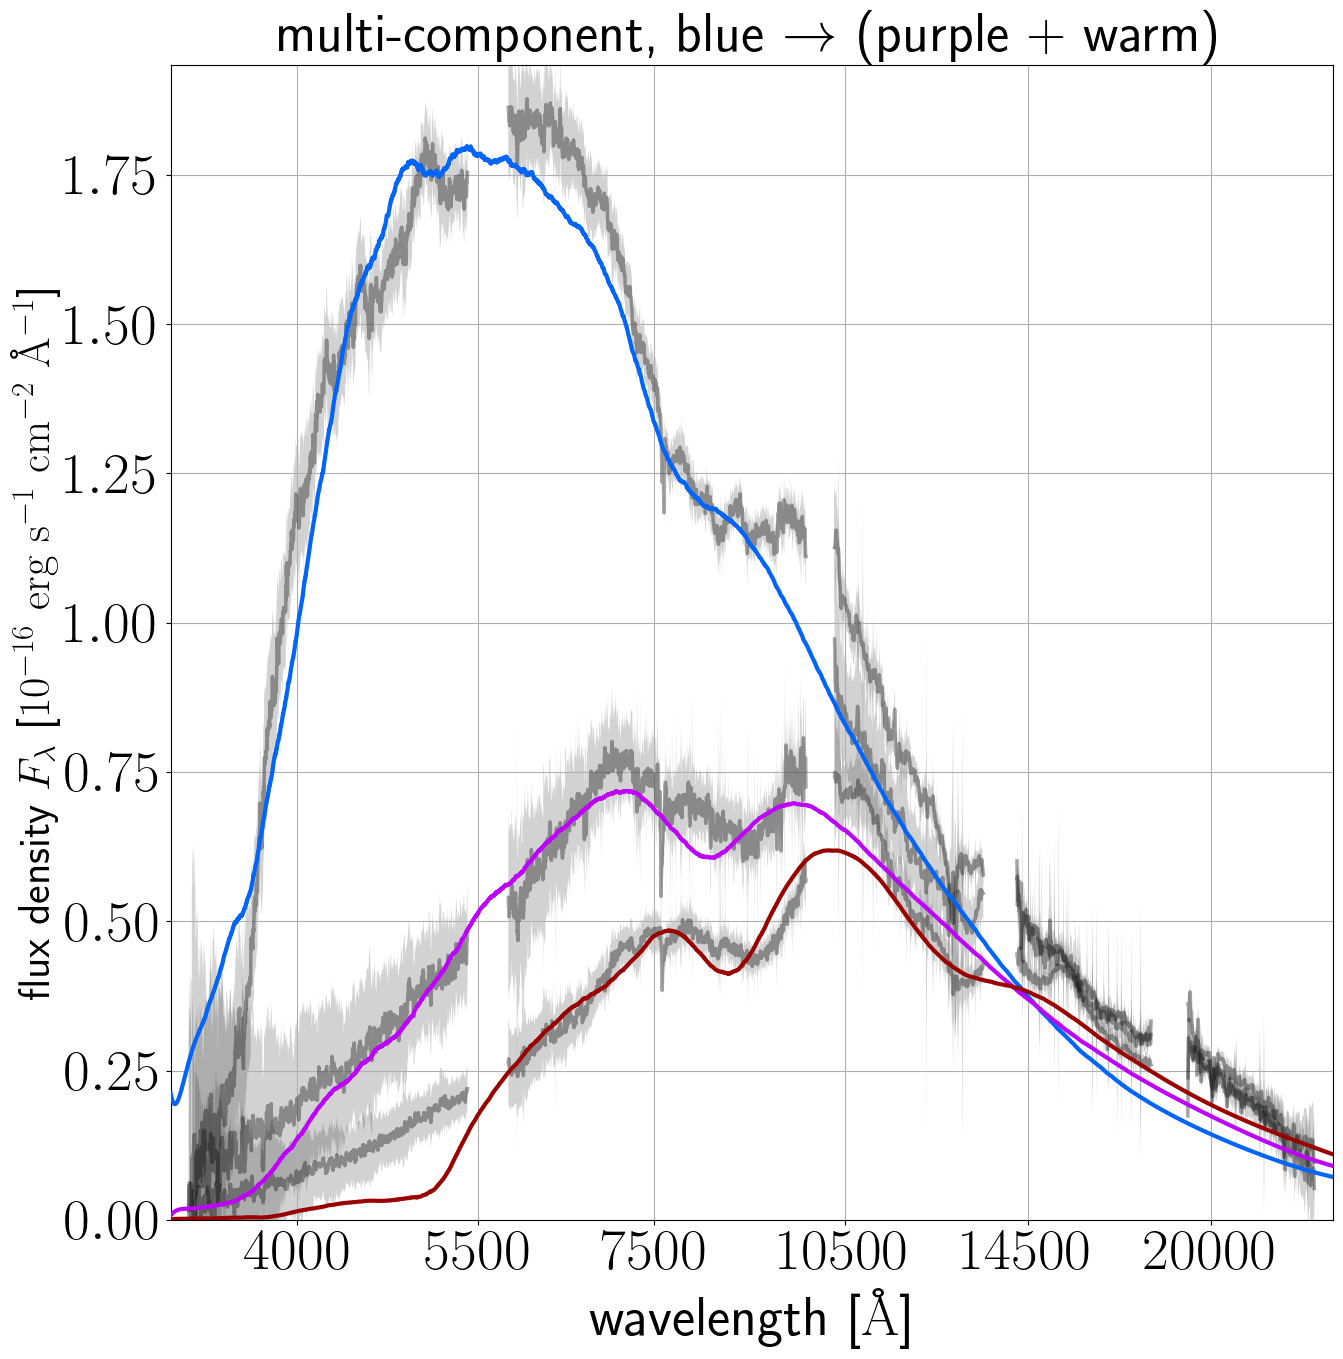
\includegraphics[width=0.4\textwidth]{figs/swap-purplewarm-multicomp_compare_all_SPARK_2.png}
    \figcaption{\textbf{Hypothetical models at 1.4, 2.4, and 3.4 days, where the bluer component of each multi-component fit has been replaced by that of the purple + warm (single-component, 1.4 days) model of V23}. Here, we take the best fit parameters from our multi-component runs (Table~\ref{tab:bestfit_multi}) and, \textit{after} fitting, swap out the bluer (higher $Y_e$) component with the purple + warm $(Y_e = 0.311,~v_{\mathrm{exp}}/c=0.240,~s / k_{\mathrm{B}}=13.6)$. Comparing to the original multi-component models (dashed lines in Figure~\ref{fig:bestfits}), the differences are negligible at all epochs.}\label{fig:swap-purplewarm}
\end{figure}

%%% FIXING the bluer component for purple+warm; Fig. 5
\begin{figure}[!t]
    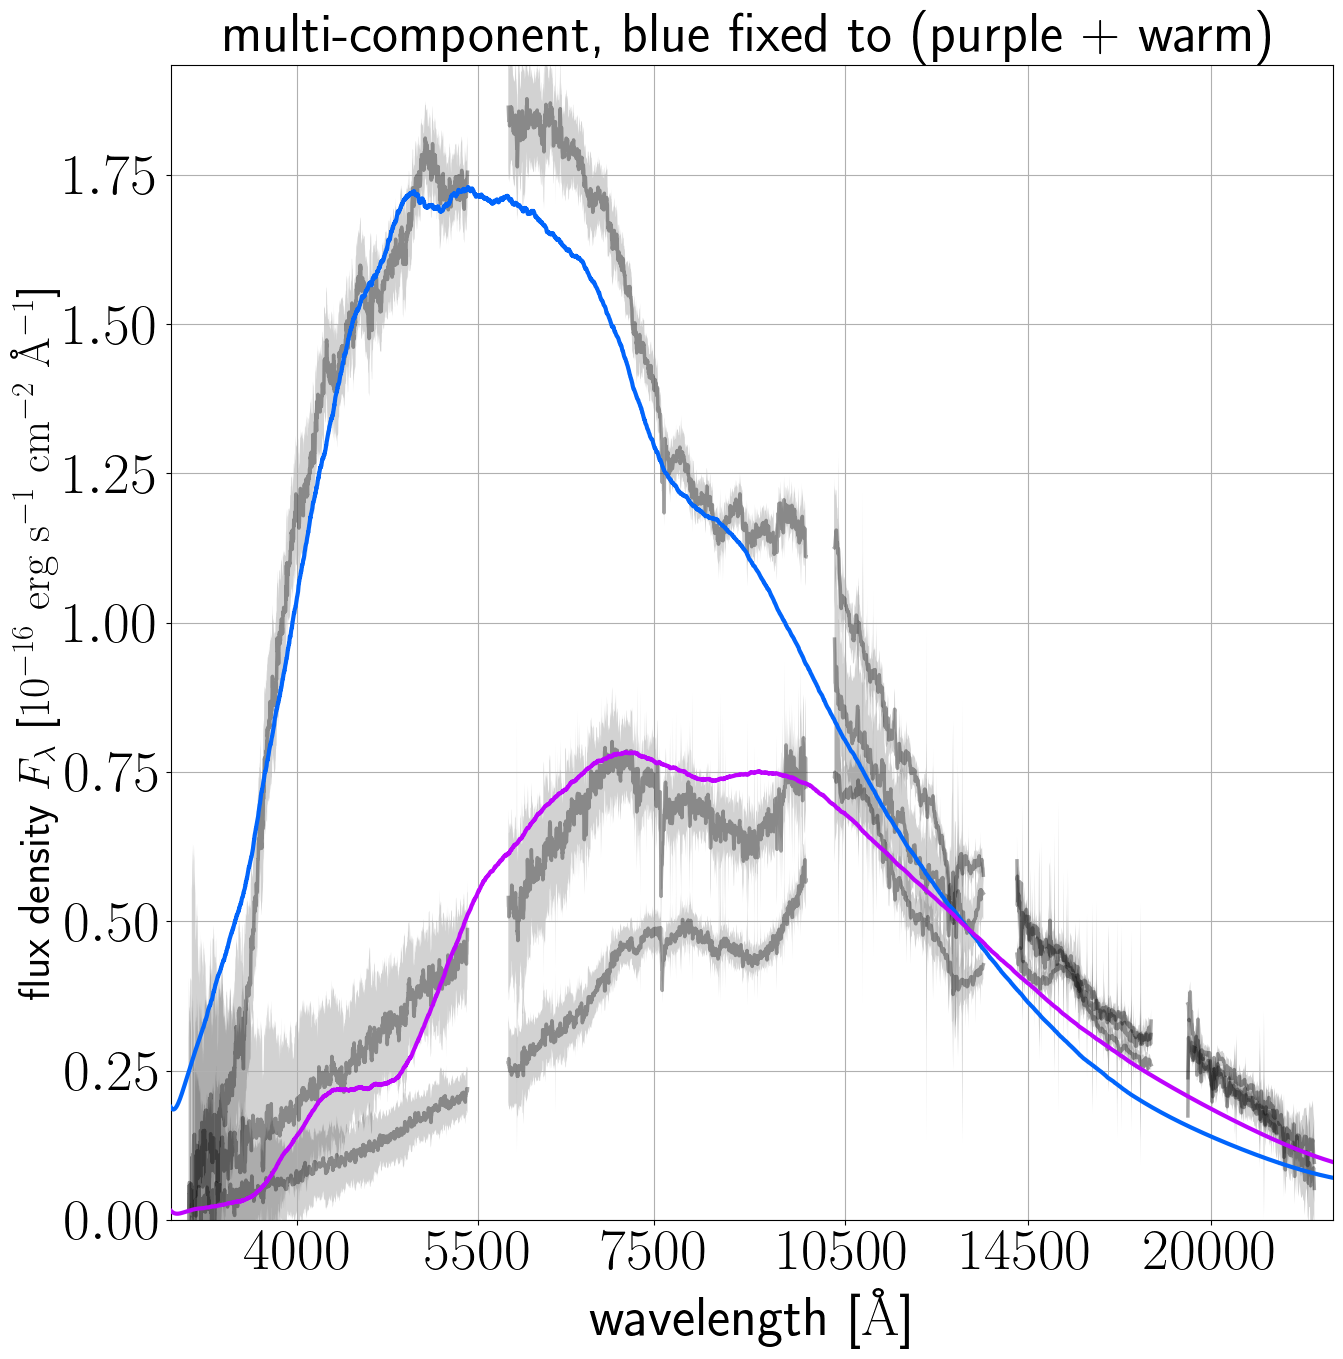
\includegraphics[width=0.4\textwidth]{figs/fix-purplewarm-multicomp_compare_all_SPARK_2.png}
    \figcaption{\textbf{Best-fit spectra at 1.4, 2.4, and 3.4 days, from multi-component \SPARK~runs where one of the two components has fixed abundance-setting parameters corresponding to the purple + warm model}. Here, we fix one of the components to the purple + warm $(Y_e = 0.311,~v_{\mathrm{exp}}/c=0.240,~s / k_{\mathrm{B}}=13.6)$, \textit{a priori}. We then run \SPARK~to obtain a new model. These fits are all disfavoured by visual inspection, compared to original multi-component models (dashed lines in Figure~\ref{fig:bestfits}). Nonetheless, these fits serve to demonstrate that the addition of a new, redder component cannot improve the fit at 1.4 and 2.4 days. \redbf{At 3.4 days...}}\label{fig:fix-purplewarm}
\end{figure}


Thus far, we have selected our favored models by visual inspection, seeing which produces a better fit to the observed spectrum at a given epoch. We have found that the 1.4 and 2.4 days spectra are well-fit by a single bluer component, whereas the 3.4 day spectrum needs an additional redder component rich in lanthanides. 

We observe that, even when allowed to yield multiple components, the multi-component \SPARK~runs yield effectively single-component best fits at 1.4 and 2.4 days. At 1.4 days, the bluer component contains $\sim$100$\times$ the mass of the redder, and the presence of the red is inconsequential. At 2.4 days, the two components are roughly equal in mass and are characterized by similar abundance patterns. 

In contrast, at 3.4 days, the two components have different abundance patterns. In particular, the role of the bluer component is to provide enough Sr to yield the $\sim$8000 \AA~absorption, while the redder yields the ensemble of lanthanides needed to produce the short-wavelength $\lesssim$7500 \AA~absorption. Given our atomic data, line list, and (most importantly) abundance patterns from the reaction network calculations of \cite{wanajo18}, no single component is able to simultaneously yield the abundance of Sr and lanthanides needed to reproduce the observed 3.4 day spectrum of AT2017gfo.

Aside from asking whether a single- or multi-component ejecta is individually preferred at each epoch, we also ask: does the \textit{addition} of a new component to the original, purple + warm ejecta at 1.4 days improve the fit? As a first test, we replace the bluer component of the multi-component models at 1.4, 2.4, and 3.4 days with this purple + warm component. (The bluer components have $Y_{e} = $ $ 0.340^{+0.022}_{-0.021}$, $0.288^{+0.129}_{-0.187}$, and $0.228^{+0.073}_{-0.088}$ at 1.4, 2.4, and 3.4 days, respectively). Figure~\ref{fig:swap-purplewarm} shows the resultant spectra. Replacing these components with the $(Y_e = 0.311,~v_{\mathrm{exp}}/c=0.240,~s / k_{\mathrm{B}}=13.6)$, there is minimal impact on the resultant spectrum and we retain a good fit.  This is not surprising at 1.4 and 2.4 days, where the inferred $Y_e$ is consistent with the purple + warm model. It is, however, surprising at 3.4 days. This further suggests that the role of the bluer component at 3.4 days is simply to provide enough Sr to produce the $\sim$8000 \AA~absorption. 

As a second, more rigorous test, we re-perform multi-component \SPARK~runs with one of the two components fixed to that of the purple + warm. Specifically, we fix $Y_{e,2} = 0.311$, $v_{\mathrm{exp},2}/c = 0.240$ and $s_2 / k_{\mathrm{B}} = 13.6$. We compile the resultant fits in Figure~\ref{fig:fix-purplewarm}. At 1.4 days, we obtain a good fit which captures most of the continuum at short wavelengths $\lesssim$5500 \AA, and the $\sim$8000 \AA~absorption. However, the absorption is somewhat underestimated, and the single-component purple + warm on its own remains the favoured model. Nonetheless, the component which is allowed to vary converges to $Y_{e,1} = 0.337^{+0.034}_{-0.027}$, and $s_1 / k_{\mathrm{B}} = 20.4^{+4.2}_{-3.9}$. This component has essentially the same abundance pattern as the purple + warm. Moreover, the two components overlap completely in space. Once again, this model is effectively single-component, demonstrating that the fit at 1.4 days cannot be improved by adding some new component to the purple + warm. At 2.4 days, we find what is generally a poor fit, but the fit captures the general shape of the continuum and some of the absorption at $\sim$8000 \AA. The component which is allowed to vary converges to $Y_{e,1} = 0.243^{+0.169}_{-0.183}$, and $s_1 / k_{\mathrm{B}} = 25.5^{+8.2}_{-11.5}$, and overlaps completely with the other component. While these parameters are consistent with those of a blue component with similar abundance pattern to the purple + warm, the broadness of the posterior and the poor fit make this agreement less significant. Nonetheless, at 2.4 days, the component allowed to vary has converged to one that completely overlaps the other and has a similar abundance pattern---again, effectively yielding a single-component ejecta. \redbf{[At 3.4 days, we find...]} 

Finally, given our Bayesian inference framework, we also use quantitative model comparison to assess how one model is favored over another. We compare the single- and multi-component models compiled in Figure~\ref{fig:bestfits}. \redbf{(Explain how we do model comparison. Will probably be something tricky)}. \redbf{(If Bayes factors are what we even use)} We find a Bayes factor  of \redbf{$X$} favoring the single- over multi-component at 1.4 days, \redbf{$X$} favoring the single- over multi-component at 2.4 days, and \redbf{$X$} favoring the multi- over single-component at 3.4 days. \redbf{This implies...}

Overall, we see that a new, redder component emerges at 3.4 days. We emphasize that arguments based on the physical properties of the components, and quantitative Bayesian model comparison, separately and independently confirm the need for a new component at 3.4 days. One of these lines of reasoning is physical, while the other is statistical. This new red ejecta component has photospheric velocity $0.21c$ and extends out to $0.35c$, suggesting that this component was in fact present at earlier epochs, but was (1) buried underneath a much brighter blue component, and (2) partially hidden below the photosphere. 





%%% === SECTION 4 === %%%
%% DISCUSSION %%

\section{Discussion}\label{sec:disco}

%%% subsection 4.1: ABUNDANCES
\subsection{Abundances of the favored models}\label{ssc:disco-abundances}

We favor the single-component models at 1.4 and 2.4 days, and multi-component model at 3.4 days. We show the abundance patterns of these favored models in Figure~\ref{fig:abunds_time_evolution}. The overall multi-component abundance pattern at 3.4 days is computed as the mass-weighted sum over all shells, including both components. 

The 1.4 and 2.4 day abundance patterns are remarkably similar, but the 2.4 day model has greater uncertainties due to the broader overall posterior. These 2.4 day abundances show evidence for $\sim 10^{-9} - 10^{-6}$ mass fractions for some of the lighter lanthanides. However, as we see in the following section, lanthanides do not leave any clear imprint on the spectrum at 2.4 days. Overall, the 1.4 and 2.4 day spectra are well-described by a single bluer component with moderate entropy. 

In contrast, the 3.4 day abundance pattern indicates the clear presence of lanthanides in the ejecta. The total lanthanide fraction (again, taken as the mass-weighted sum over all shells, including both components) is $\log_{10} X_{\mathrm{lan,total}} = -0.97^{+0.23}_{-0.32}$. Nonetheless, the bluer component of this multi-component ejecta provides Sr, the role of which is crucial, as seen in the following section. Indeed, we infer abundances of $Y_{\mathrm{Sr},1.4} = 0.069^{+0.021}_{-0.010}$ and $Y_{\mathrm{Sr},2.4} = 0.087^{+0.060}_{-0.020}$ at 1.4 and 2.4 days, and $Y_{\mathrm{Sr},3.4} = 0.067^{+0.035}_{-0.002}$ (mass-weighted sum over all shells, including both components) at 3.4 days. These are remarkably consistent with each other.

The inferred abundance patterns at 1.4 and 2.4 days are markedly non-Solar, where the Solar $r$-process abundance pattern is taken using the data of \cite{lodders09} with the $s$-process residuals subtracted according to \cite{bisterzo14}. If all NS-NS/BH mergers produced such blue ejecta, this would point to the inability of these mergers to yield the $r$-process abundances seen in several astrophysical settings. However, the 3.4 days abundance pattern is much closer to Solar, up to $Z \sim 80$. In particular, the presence of lanthanides improves this agreement. % In the following section, we examine the role of individual elements and ions, including these lanthanides. 




%%% subsection 4.2: LoO AND SDEC
\subsection{Elements \& ions present in the favored models}\label{ssc:disco-elements}


%%% leave-one-out spectra; Fig. 5
\begin{figure}[!ht]
    \centering
    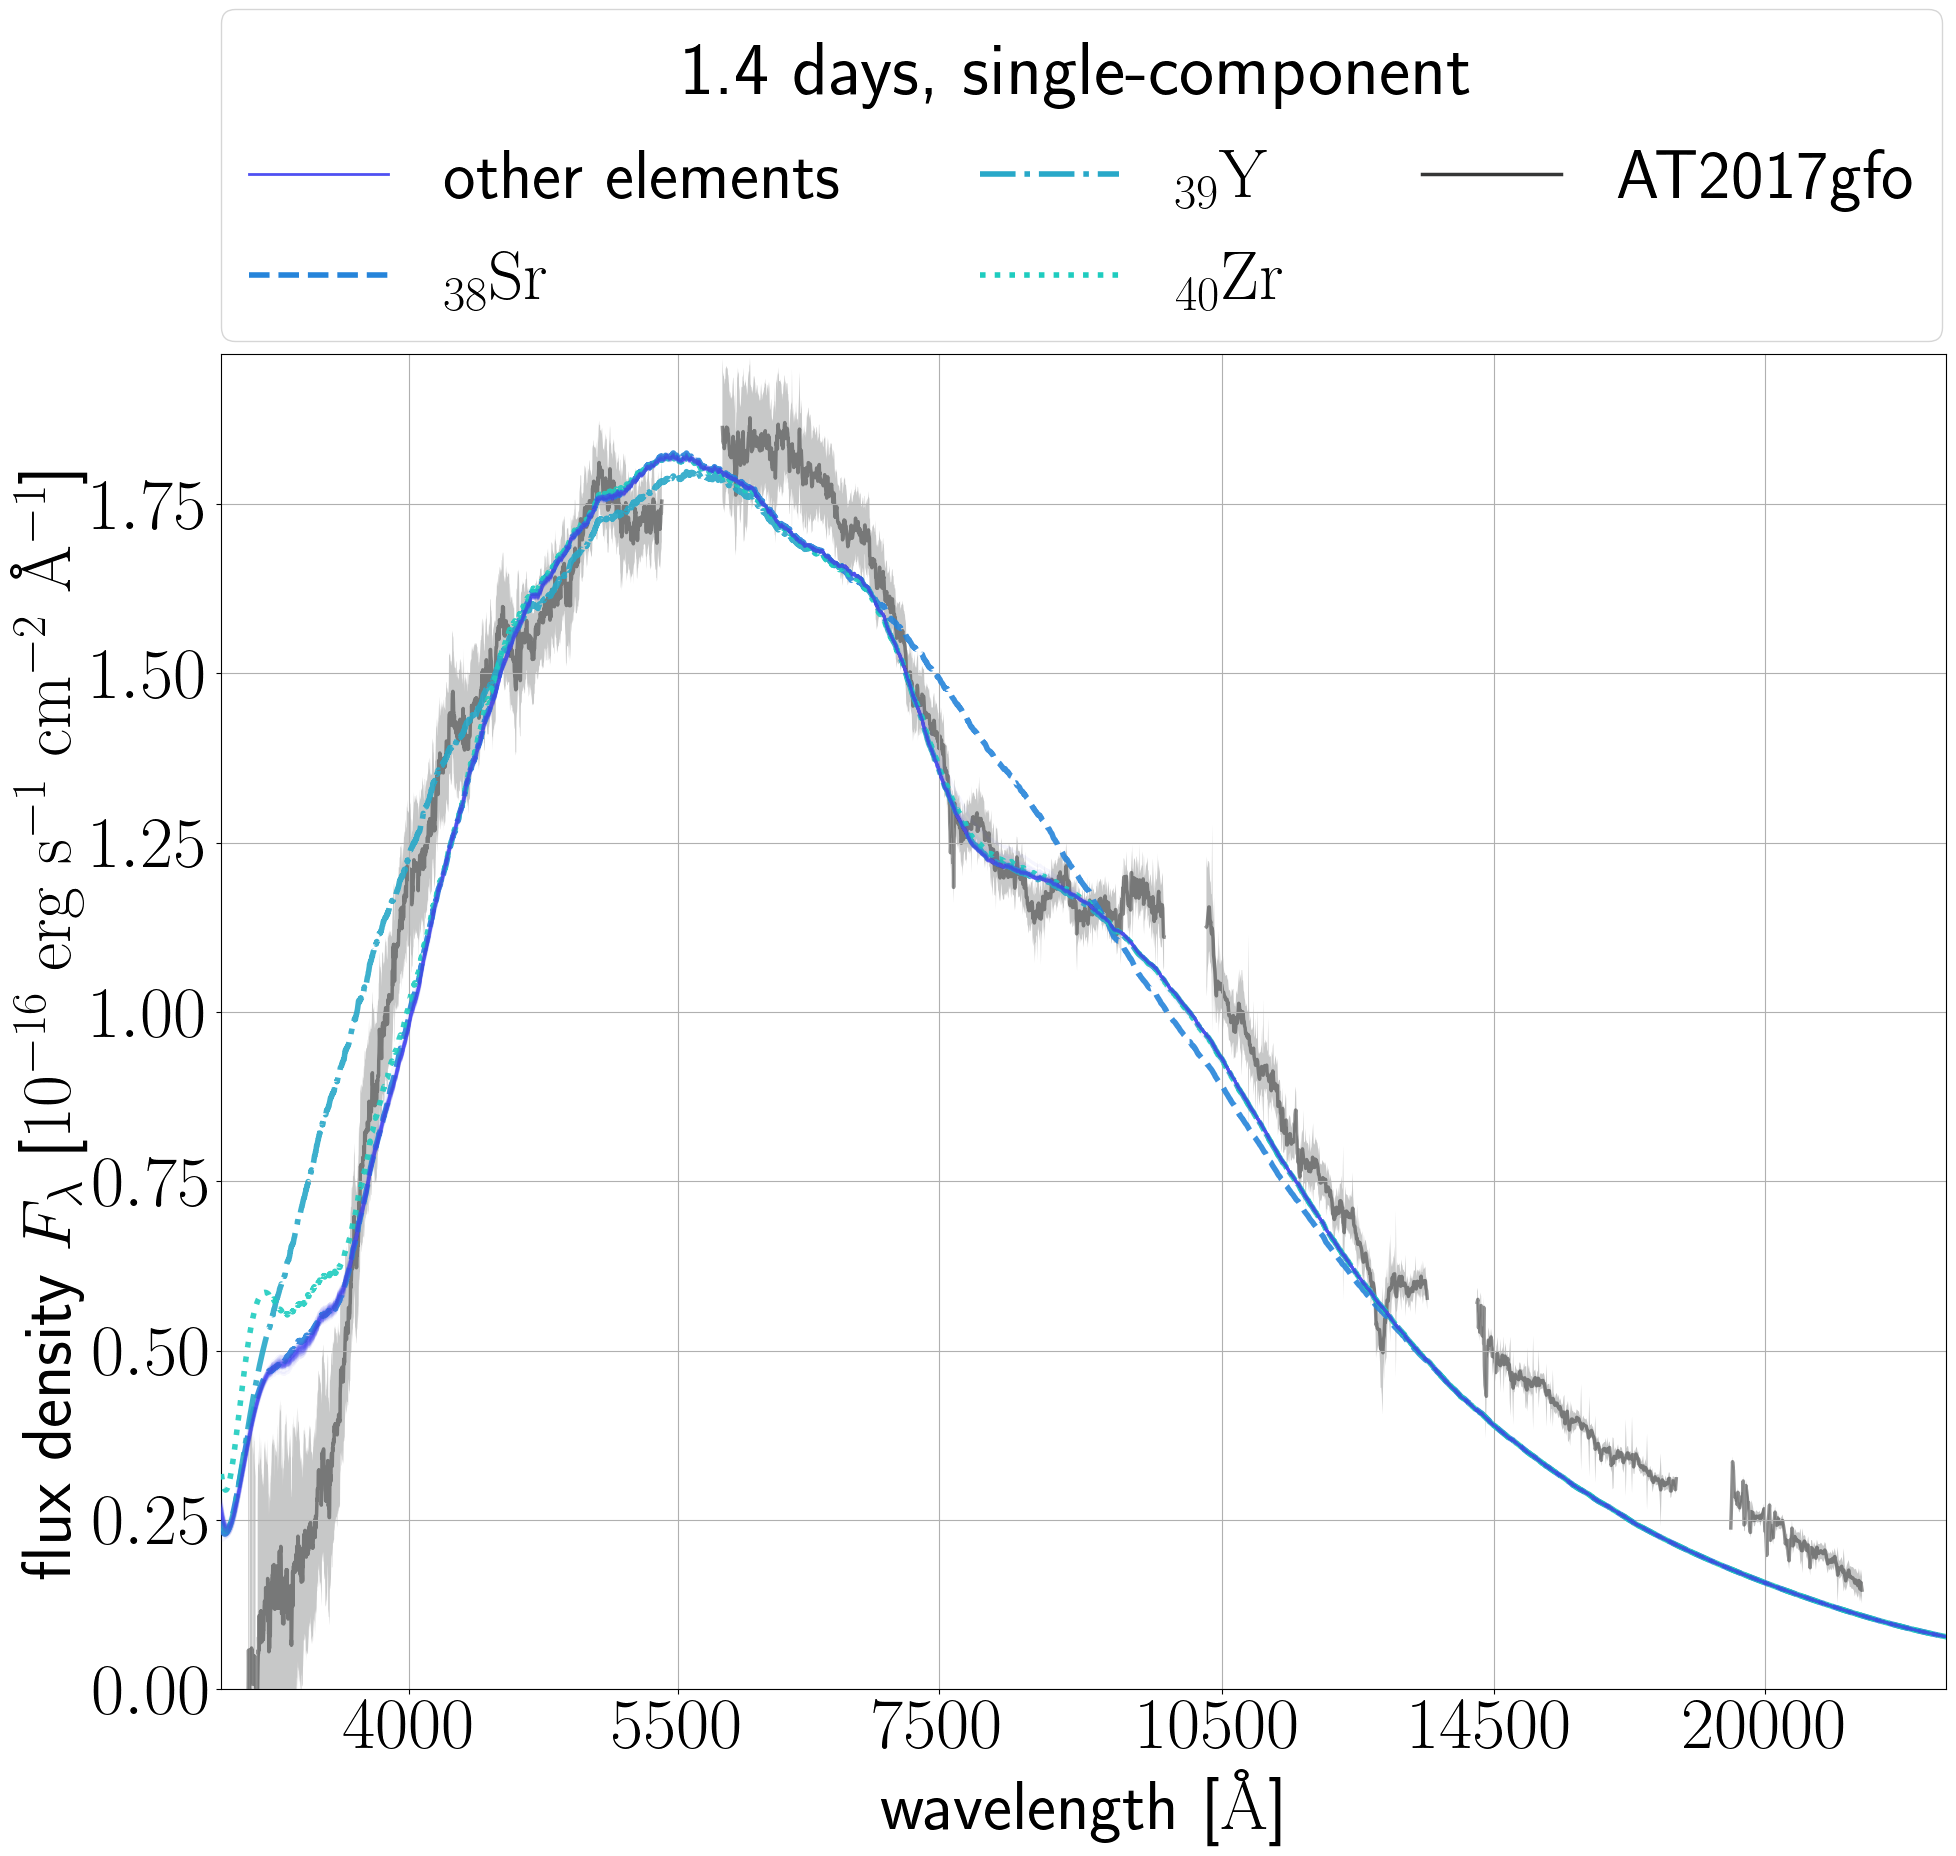
\includegraphics[width=0.35\textwidth]{figs/220816_130039_leaveoneout_all_TARDIS_evals_label-interest-38-39-40.png}
    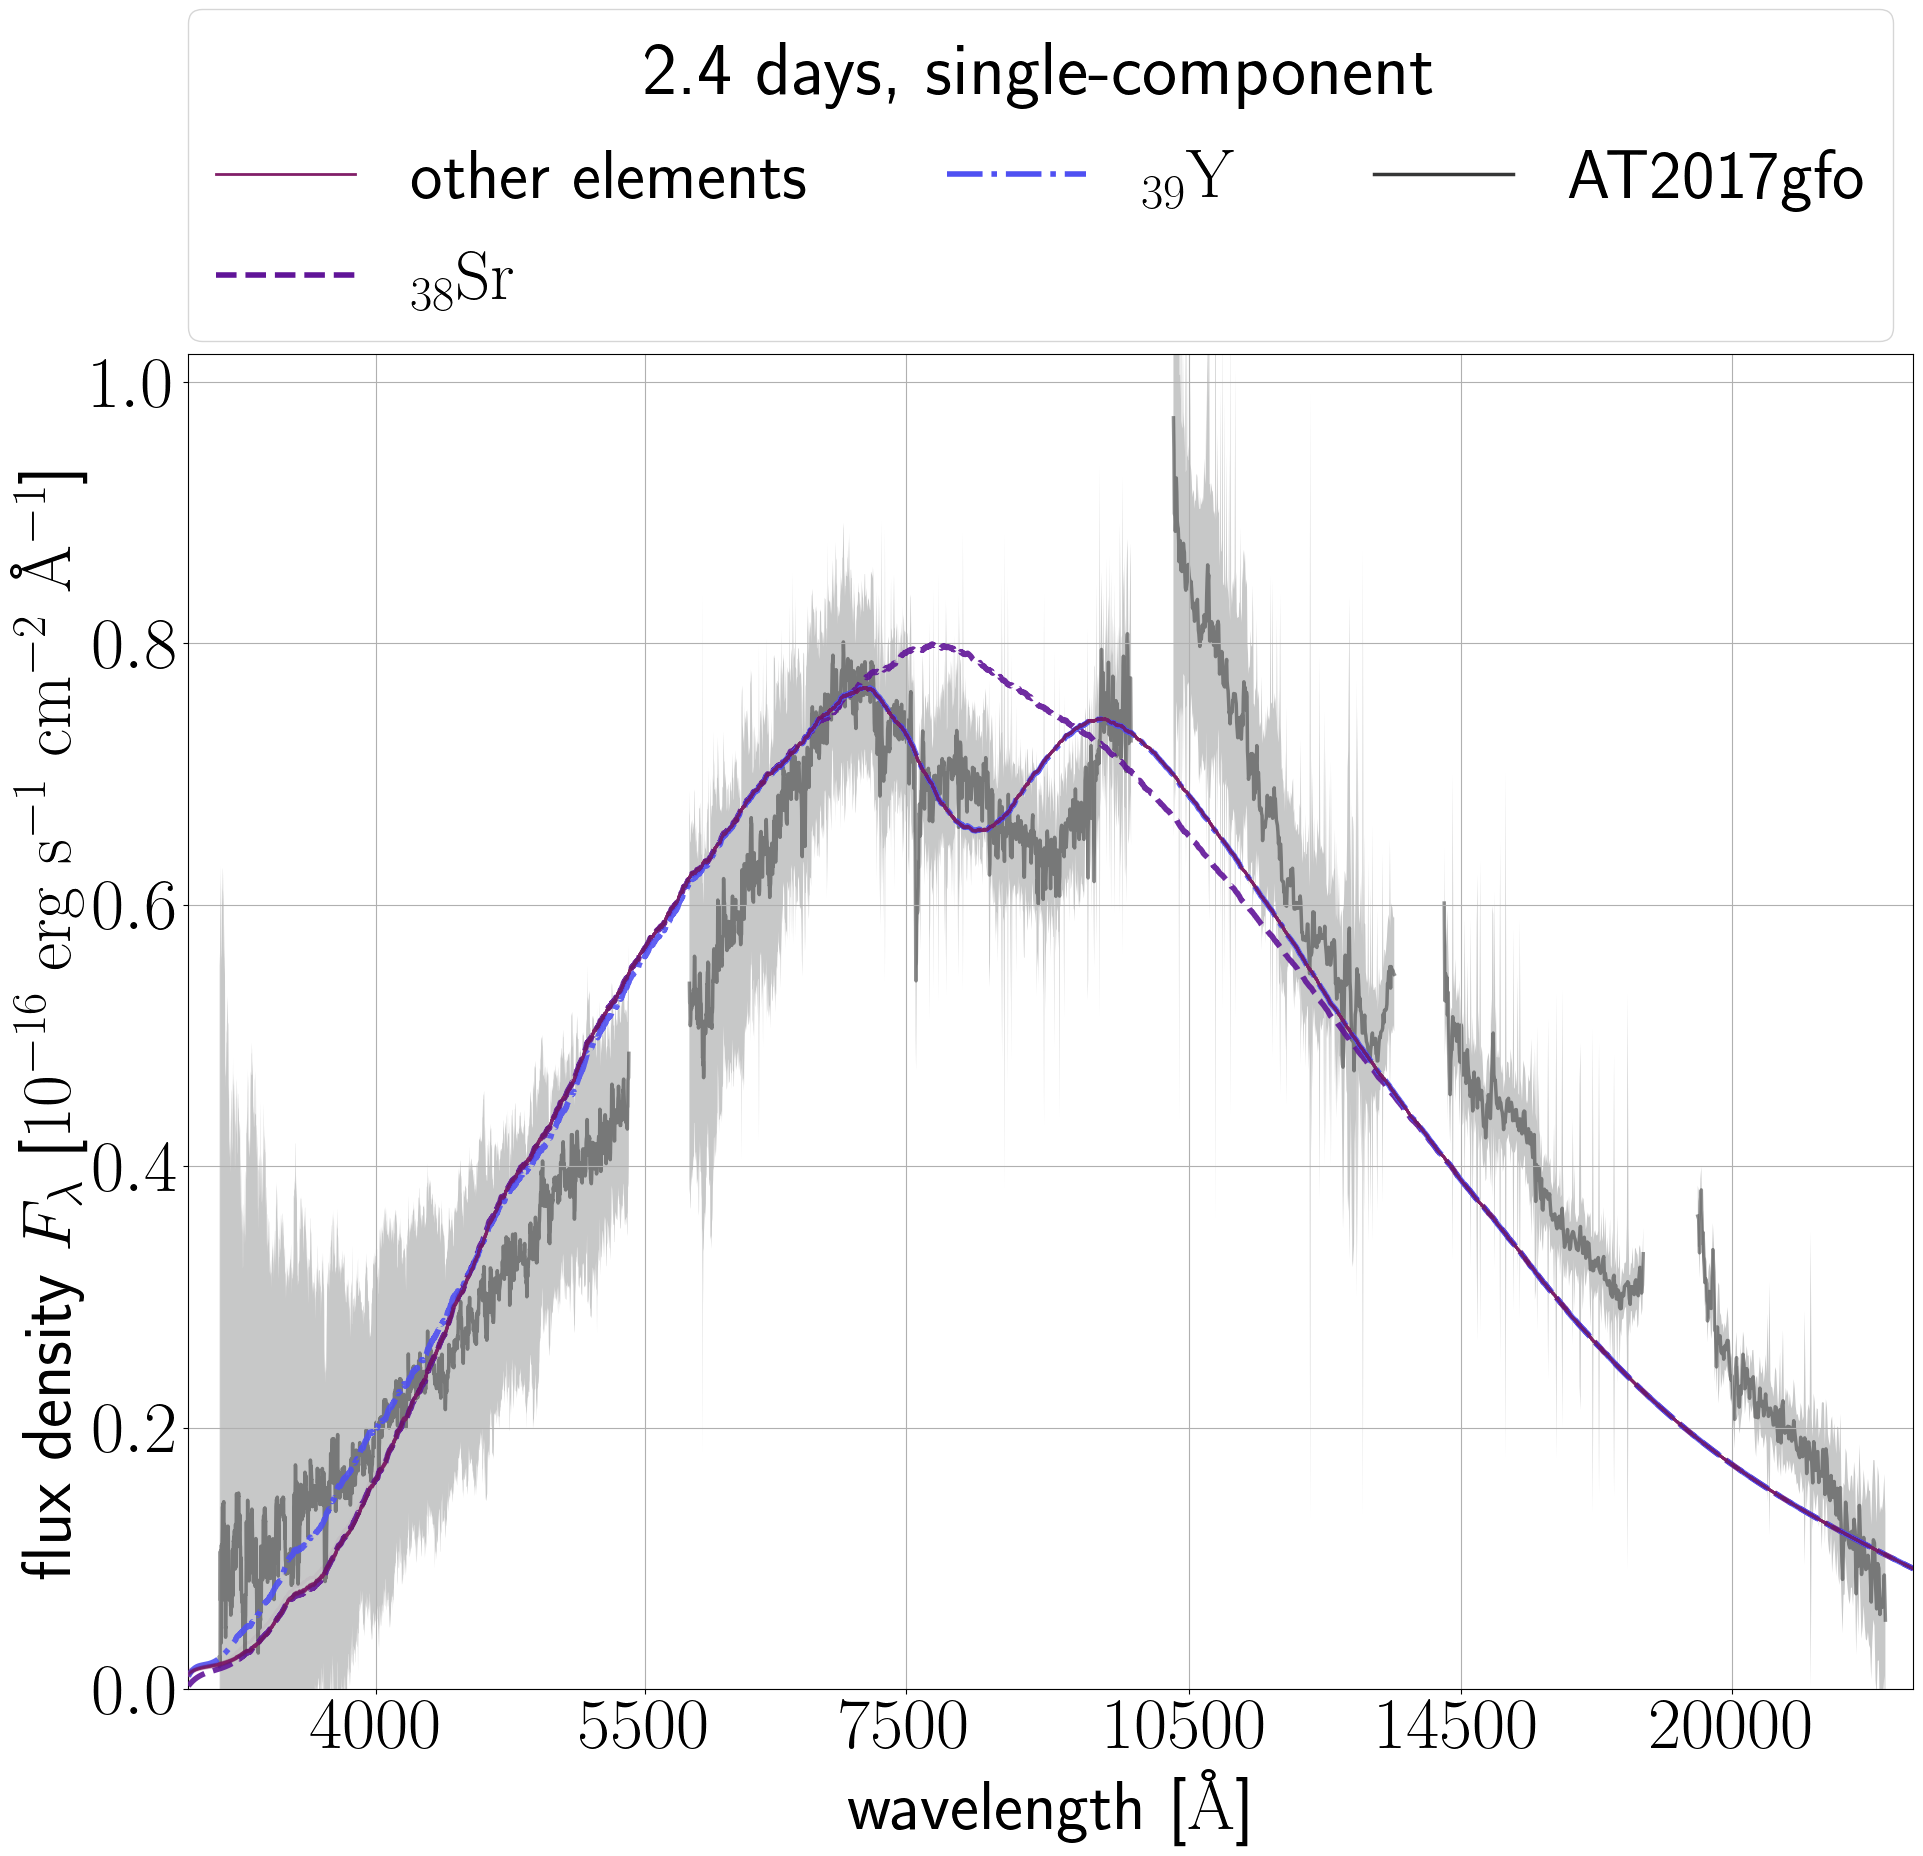
\includegraphics[width=0.35\textwidth]{figs/230409_234104_leaveoneout_all_TARDIS_evals_label-interest-38-39.png}
    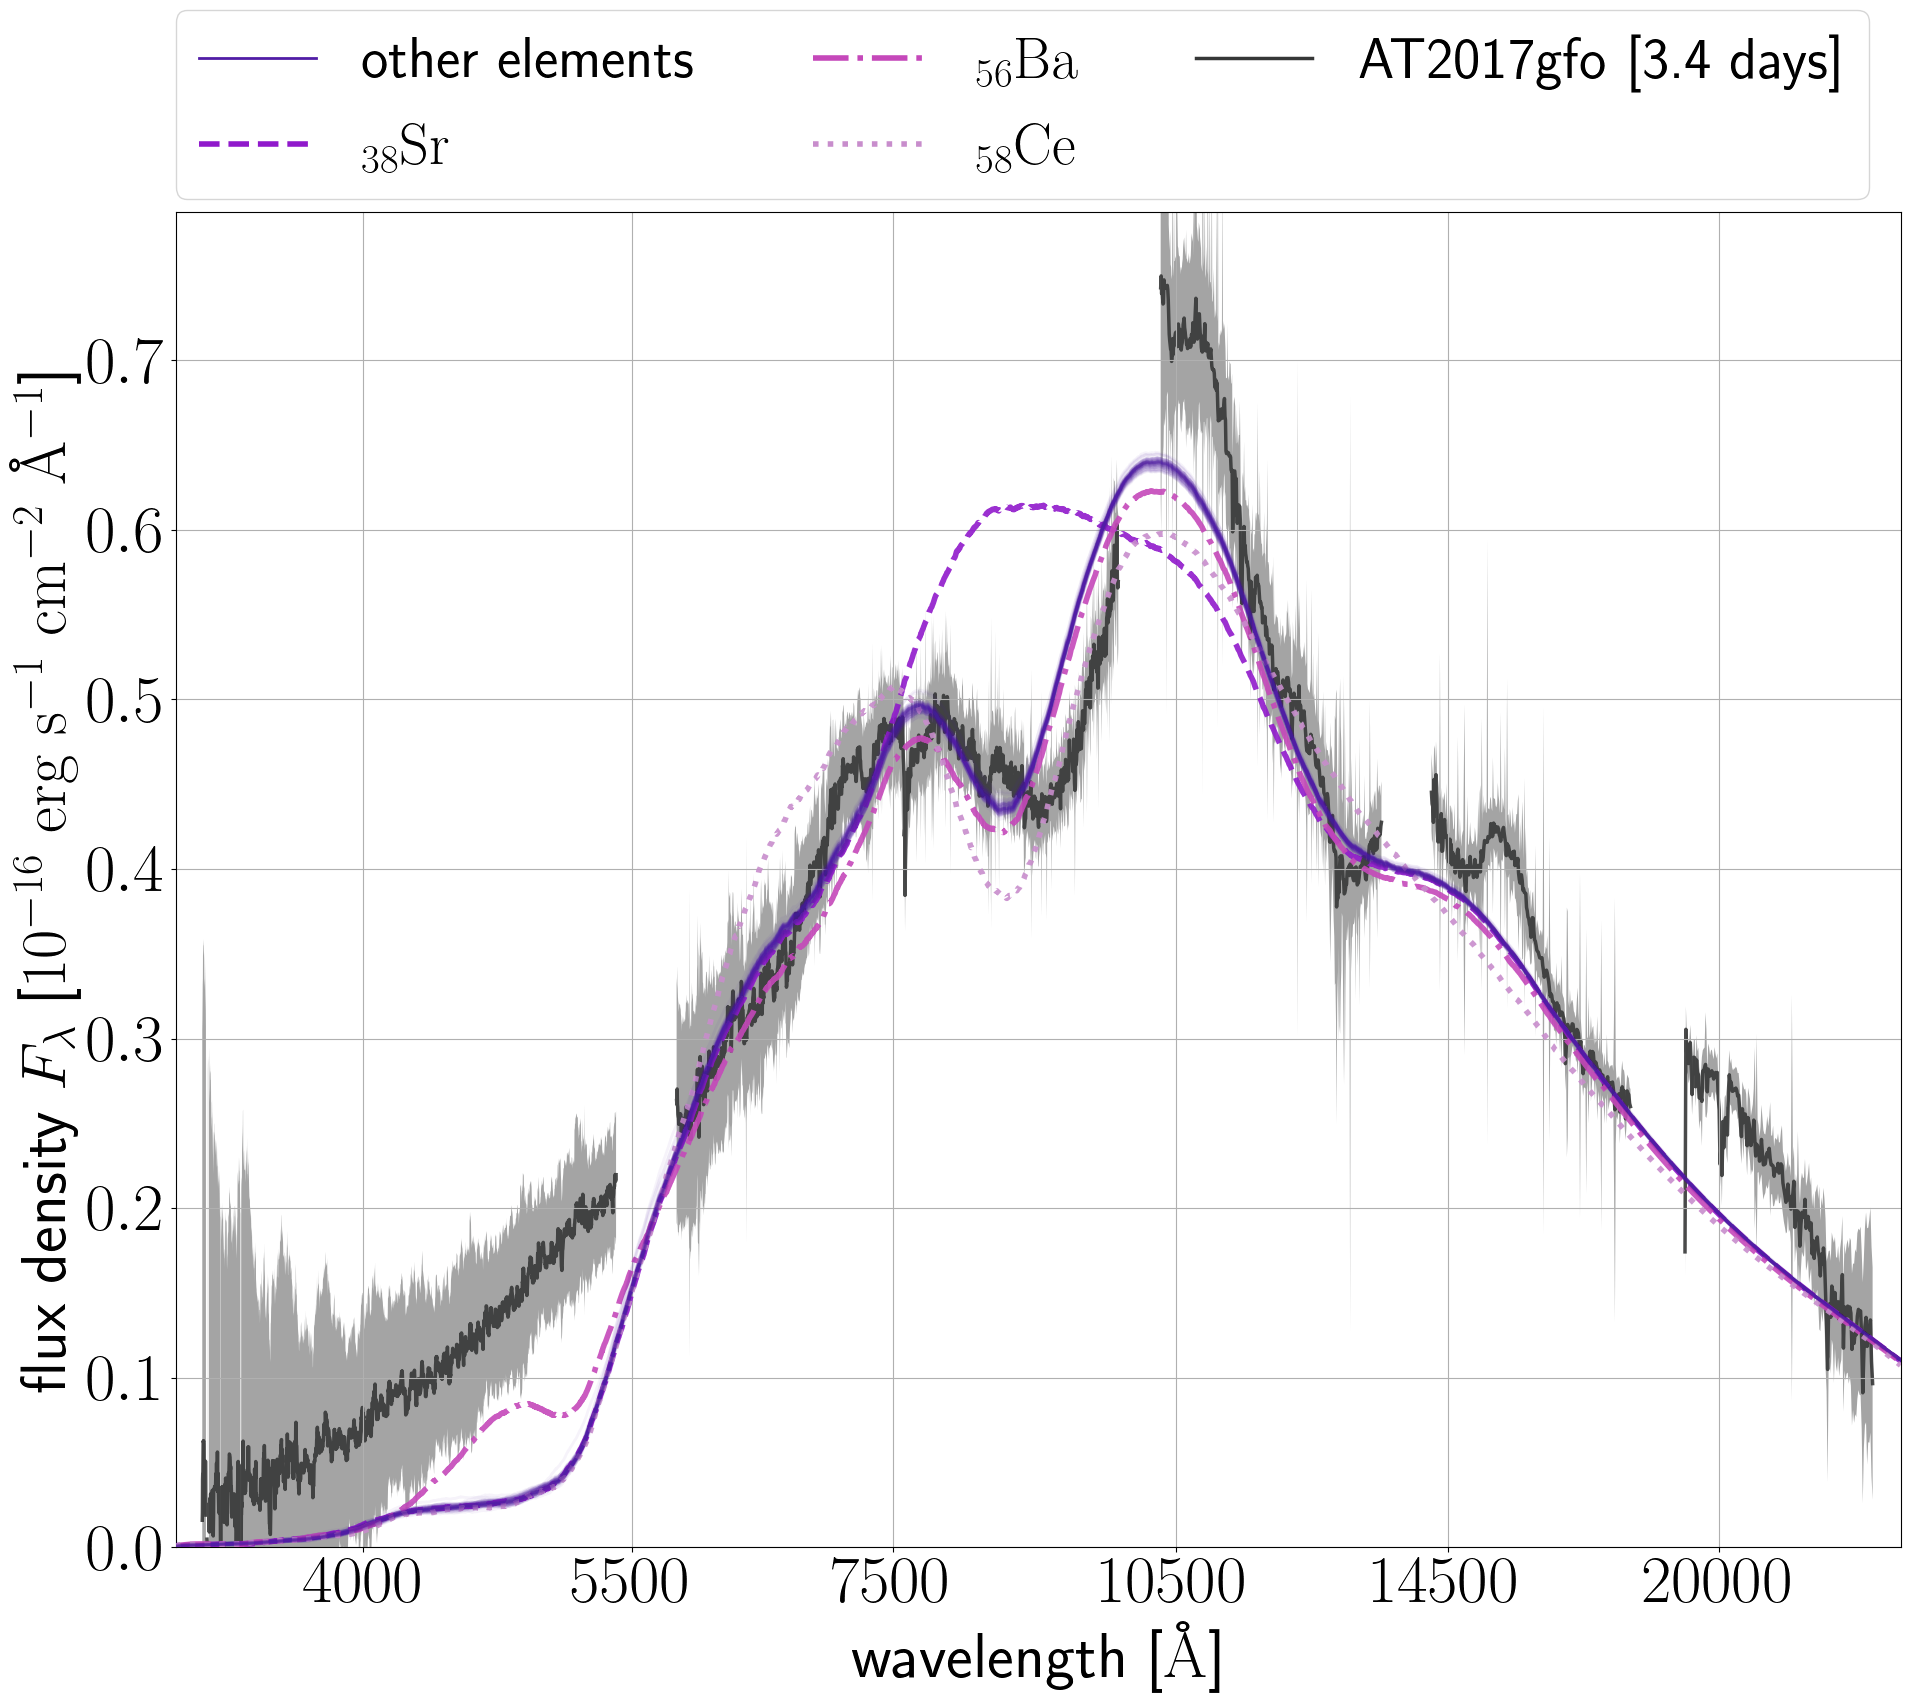
\includegraphics[width=0.35\textwidth]{figs/230626_170245_leaveoneout_all_TARDIS_evals_label-interest-38-56-58.png}
    \figcaption{\textbf{Leave-one-out spectra for the favored models: single-component for 1.4 (\textit{top}) and 2.4 (\textit{center}) days, and multi-component for 3.4 days \textit{(bottom)}.} All models show clear absorption from strontium (${}_{38}$Sr) at $\sim$8000 \AA. At 3.4 days, when the abundances includes heavier elements, we see an over-absorption from barium (${}_{56}$Ba) at $\sim$4500\AA. We also see absorption (at $\sim$7000 \AA~and $\sim$12,000 \AA) and emission (at $\sim$8000 \AA) from the lanthanide cerium (${}_{58}$Ce) at this epoch. Spectral DEComposition (SDEC) plots, included in Appendix~\ref{app:SDEC}, provide a complementary view of the dominant species.}\label{fig:leaveoneout_pref}
\end{figure}


To assess the impact of different elements on the best fits, we generate leave-one-out spectra. In each, we iteratively leave out a single element by setting its abundance to 0 and transferring that original abundance to a filler element. We use helium (He) as our filler element, since it should not have a marked impact on the emergent spectrum when the ejecta remains optically thick and local thermodynamic equilibrium (LTE) is a valid approximation (\citealt{perego22, tarumi23}).

In Figure~\ref{fig:leaveoneout_pref}, we show leave-one-out spectra for the new favored models at 2.4 and 3.4 days, and the 1.4 day model from V23. We see the clear imprint of Sr at $\sim$8000 \AA~at 1.4, 2.4, and 3.4 days. This is in line with \cite{watson19, gillanders22, domoto21, domoto22, sneppen23, sneppenwatson23}, and V23, which all argue for the importance of Sr in the spectra. 

At 2.4 days, we also see evidence for absorption from yttrium (${}_{39}$Y) at short wavelengths, as we have at 1.4 days in V23. This identification at 2.4 days strengthens our previous claim of the importance of Y, and is in agreement with \cite{gillanders22}, which identified Y at these early epochs. Interestingly, Y does not have the same pronounced impact at 3.4 days. This is in agreement with \cite{sneppenwatson23}, which finds that absorption from Y is less prominent at 3.4 days, before a P Cygni feature emerges at $\sim$7600~\AA~at 4.4 and 5.4 days. In our favored multi-component model, the absorption from the lanthanides is much stronger at these (and shorter) wavelengths. 

At 3.4 days, we identify two new, heavier elements: barium (${}_{56}$Ba), an open $s$-shell element in the same periodic table group as Sr, and cerium (${}_{58}$Ce), a lanthanide. Ba is actually responsible for some of the \textit{over}estimated absorption at $\lesssim$5000 \AA. This overestimated absorption is more severe in the multi-component model than in the single-component, but recall that we neglect wavelengths $\leqslant$6400 \AA~in our computation of the likelihood at 3.4 days to obtain a fit which accurately captures the Sr absorption. Some of the overestimated Ba absorption is re-processed and emitted at $\sim$8000 \AA, but, overall, the omission of Ba improves the fit. This suggests that we overestimate the abundance of Ba in our best fit abundance pattern. The other new element, Ce, produces absorption at $\sim$7000 \AA~which is re-processed and emitted at $\sim$8000 \AA, and its omission worsens the fit. Ce also introduces some absorption at $\sim$12,000 \AA. Interestingly, this absorption may originate from astrophysically-measured \ion{Ce}{2} lines in the range of $\sim$$15,200 - 16,700$ \AA~(\citealt{cunha17, majewski17}), blue-shifted due to the expansion of the ejecta. \cite{domoto21} similarly noted that these \ion{Ce}{2} lines may be prominent in kilonova spectra.

We complement these leave-one-out analyses using the Spectral DEComposition (SDEC) tool of \TARDIS. SDEC allows us to measure which elements or ions absorb the greatest luminosity during a given \TARDIS~run. All SDEC plots, for favored and disfavored models, are compiled in Appendix~\ref{app:SDEC}. In both single- and multi-component models at 1.4 days, we see that the absorption of photon packets is dominated by just three singly-ionized species: \ion{Sr}{2}, \ion{Y}{2}, and \ion{Zr}{2}. Indeed, 98.9\% and 83.4\% of all absorbed luminosity is absorbed by just these three species, in the single- and multi-component models, respectively. These ions remain important at 2.4 days, though the impact of \ion{Zr}{2} is less clear. We also see some light absorption from \ion{Ba}{2} at 2.4 days, at the shortest wavelengths. This is more clear in the multi-component model, but the single-component model is favored.

At 3.4 days, the SDEC plots reveal the presence of several new ions. \ion{Sr}{2} remains important, but singly-ionized species of heavier elements also emerge. In the favored multi-component model, we see clearer evidence for \ion{Ba}{2}, with the caveat that the abundance of Ba is likely overestimated. More interesting, we see absorption from four singly-ionized lanthanides: \ion{Ce}{2}, \ion{Nd}{2}, \ion{Sm}{2}, and \ion{Eu}{2} (cerium, ${}_{58}$Ce; neodymium, ${}_{60}$Nd; samarium, ${}_{62}$Sm; europium, ${}_{63}$Eu). While none of these species except \ion{Ce}{2} contribute enough absorption to emerge on their own in the leave-one-out spectra, altogether, \ion{Ce}{2}) is responsible for 27.5\% of the absorbed luminosity at this epoch, and \ion{Nd}{2} + \ion{Sm}{2} + \ion{Eu}{2} are responsible for 20.4\%, compared to 30.3\% from \ion{Sr}{2}. This is a clear indication of the presence of lanthanides in the ejecta. Interestingly, Eu is a ``pure'' $r$-process element, in that it is produced in negligible quantities by the $s$-process (\textit{e.g.}, \citealt{bisterzo14}). The presence of Eu is thus further proof for the operation of the $r$-process in NS-NS merger ejecta. Finally, at 3.4 days, we also see some light (5.2\% of the total) absorption from an ion of bismuth, \ion{Bi}{2}. This is the heaviest element ($Z=83$) detected in any of our models, but we caution that its detection is marginal (we measure an abundance of $Y_{\mathrm{Bi},3.4} = 7.84^{+24.6}_{-7.43} \times 10^{-6}$) and it does not leave a clear imprint on the leave-one-out spectra. 

Considering both the leave-one-out and SDEC analyses, we confidently identify Sr at all epochs. We solidify our identification of Y at 1.4 and 2.4 days. Ba may also be present in the ejecta, but its abundance is likely overestimated at 3.4 days, complicating this claim. Finally, at 3.4 days, we infer the presence of singly-ionized species of the lanthanides Ce, Nd, Sm, and Eu, with the detection of Ce being most concrete. At 3.4 days, the ejecta has evolved to expose a much redder, lanthanide-rich component which was not needed to fit the earlier spectra at 1.4 and 2.4 days.



%%% subsection 4.3: PHYSICAL ORIGIN OF EJECTA COMPONENTS
\subsection{Physical origin of the ejecta components}\label{ssc:disco-origins}

 Given the inferred electron fraction and entropy (we neglect expansion velocity, since it is poorly constrained), the ejecta at 1.4 and 2.4 days is consistent with a viscously driven outflow from a remnant accretion disk. At 3.4 days, the bluer component ($Y_{e,1} = 0.228^{+0.073}_{-0.088}$, $s / k_{\mathrm{B}} = 14.9^{+8.0}_{-4.5}$), is consistent with \redbf{[some other component with ($Y_e \sim 0.23$, $s / k_{\mathrm{B}} \sim 15$)]} \citneeded . However, this component can also be replaced with the purple + warm model of 1.4 days, which is consistent with an outflow from an accretion disk, without significantly changing the fit (see Figure~\ref{fig:swap-purplewarm}). The redder component ($Y_{e,2} = 0.161^{+0.149}_{-0.104}$, $s / k_{\mathrm{B}} = 21.5^{+8.3}_{-9.5}$) is better matched to \redbf{[some other component with ($Y_e \sim 0.16$, $s / k_{\mathrm{B}} \sim 22$)]} \citneeded . \redbf{[Interpretation here...]}

 The mass ratio of the redder over the bluer component at 3.4 days (equivalently, the mass ratio of the \redbf{[some other component with ($Y_e \sim 0.16$, $s / k_{\mathrm{B}} \sim 22$)]} over the mass of the disk wind) is $M_1 / M_2 = 1.42^{+0.14}_{-0.14}$. \redbf{[This is or isn't consistent with...]}




% %%% subsection 4.4: CONSISTENCY WITH PHOTOMETRIC ANALYSES
% \subsection{Consistency with light curves}\label{ssc:disco-lightcurves}

% \redbf{May or may not do this depending on time. Idea: convolve our best fit spectra with various filters and produce light curves. See if these light curves are consistent with the various components reported in \cite{villar17}.}




%%% === SECTION 5 === %%%
%% CONCLUSIONS %%
\section{Conclusions}\label{sec:conco}

We fit single- and multi-component ejecta models to the spectra of the GW170817 kilonova, AT2017gfo, during the early, optically thick phase: 1.4, 2.4, and 3.4 days post-merger. With these fits, we infer the element-by-element abundance patterns, with uncertainties, at each of these epochs. Using both physical argument and quantitative model comparison, we find that a single-component model is favored at 1.4 and 2.4 days, while a multi-component model is favored at 3.4 days. 

This single component at 1.4 and 2.4 days is blue, characterized by an electron fraction $Y_e = 0.3$, and moderate specific entropy per nucleon $s / k_{\mathrm{B}} = 13 - 18$. At 3.4 days, we find a bluer (but less so than earlier epochs; $Y_e = 0.23$) and redder component ($Y_e = 0.16$), with entropies in the range $s / k_{\mathrm{B}} = 15 - 22$. At 3.4 days, the photosphere has receded into the ejecta, from $0.31c$ at 1.4 days, to $0.25c$ at 2.4 days, to $0.21c$ at 3.4 days. The recession of the photosphere, and the dimming of the blue component, reveals this new redder component which was not inferred at earlier epochs. The emergence of a new red component at 3.4 days is in line with photospheric modelling of the kilonova. This new redder component is rich in lanthanides, which provide absorption in the spectrum at $\lesssim$7500~\AA. Strontium (${}_{38}$Sr) remains present in the blue component, and provides the $\sim$8000~\AA~absorption, in agreement with other spectroscopic studies. The combination of two components---one rich in strontium and poor in lanthanides, the other the opposite---is needed to reproduce the observed spectrum at 3.4 days.

Aside from finding Sr at each epoch, we also strengthen our identification of yttrium (${}_{39}$Y) at short wavelengths $\lesssim$4500~\AA~at 2.4 days. At 3.4 days, this absorption from Y is less clear, as absorption from an ensemble of lanthanides (cerium, ${}_{58}$Ce; neodymium, ${}_{60}$Nd; samarium, ${}_{62}$Sm; europium, ${}_{63}$Eu) dominates the absorption at these short wavelengths. The identification of Ce is most concrete, producing absorption at $\sim$7000~\AA~and $\sim$12,000~\AA~and emission at $\sim$8000~\AA.

The abundance patterns at 1.4 and 2.4 days show a dearth of lanthanides and heavier elements which makes these inconsistent with the Solar $r$-process abundance pattern. The blue component at these epochs is consistent with a viscously-driven wind from a remnant accretion disk. At 3.4 days, the emergence of the lanthanide-rich red component---which leads to an overall lanthanide fraction of $X_{\mathrm{lan}} = -0.97$---substantially improves the agreement between the inferred abundance pattern and the Solar $r$-process. This new red component is consistent with \redbf{[some other component]}. The better agreement between the Solar $r$-process and inferred abundance pattern at 3.4 days, and the possible presence of multiple components (disk wind and \redbf{[some other component]}), lends more credence to the ability of NS-NS/BH mergers to yield the Universal $r$-process abundances seen in several other systems.

While we have fit at 1.4, 2.4, and 3.4 days, observations of AT2017gfo extend to later epochs. At these epochs, the ejecta may leave the photospheric phase and enter the so-called ``nebular'' phase. At this time, non-LTE effects may be non-negligible. Given the modular nature of \SPARK, it would be possible to swap our \TARDIS~for a code specifically suited to nLTE, or, use the nLTE functionality already available in \TARDIS. The Bayesian framework would also enable quantitative model comparison between models with and without nLTE effects at epochs where their importance is not yet understood (\eg, 4.4, 5.4 days). 

Finally, the inferences here are reliant on atomic/nuclear physics inputs, namely, a list of lines and nuclear reaction network calculations which map elemental abundances to relevant kilonova parameters. These reaction network calculations in turn rely on nuclear physics such as the nuclear mass model employed. Future work could explore the impact of different nuclear physics inputs on the inferred parameters, abundance patterns, and dominant species in the spectra. 

% \begin{itemize}
    
%     \item We fit single- and multi-component models to the spectra of the GW170817 kilonova, AT2017gfo, during the early, optically thick phase of the ejecta: 1.4, 2.4, and 3.4 days post-merger. We infer the element-by-element abundance patterns, with uncertainties, at each of these epochs. 

%     \item We find that the ejecta at 1.4 and 2.4 days is well-fit with a single, blue ($Y_e = 0.3$) component. At 3.4 days, we find that the spectrum is best fit with multiple components: one bluer ($Y_e = 0.23$) component which contains sufficient strontium to produce the $\sim 8000$ \AA~absorption, and another redder ($Y_e = 0.16$) which contains sufficient lanthanides for the $\leqslant 7500$ \AA~absorption. 

%     \item We find that strontium is important at all epochs. We also strengthen our identification of yttrium. Finally, we find that the 3.4 day ejecta must contain lanthanides: we specifically identify cerium, neodymium, samarium, and europium, with cerium being the most impactful. This new lanthanide-rich component at 3.4 days, with $\log_{10} X_{\mathrm{lan}} = -0.97$, is more consistent with the Solar $r$-process abundance pattern.

%     \item The bluer components present at 1.4 and 2.4 days are consistent with a viscously-driven accretion disk wind. At 3.4 days, the bluer component is consistent with \redbf{[some other component]}, though it can be replaced with that of 1.4 days without severely impacting the spectrum. The new redder component is consistent with \redbf{[some other component].}

%     \item Potential future direction: fit the 4.5, 5.5, etc. epochs

%     \item Potential future direction: by connecting our inference to reaction network calculations, we have also effectively inferred the heating rate. Can we use this to try to fit light curves and check for consistency with photometric analyses?

%     \item Potential future direction: replace \TARDIS~with some nLTE code, extend \SPARK~to the post-photospheric (nebular) epochs

%     \item Potential future direction: assess the impact of different nuclear physics (most likely nuclear mass models) and the resultant reaction networks on spectral synthesis / inference

% \end{itemize}





%%% === ACKNOWLEDGEMENTS === %%%
\acknowledgments


NV works in Tiohti{\'a}:ke / Mooniyang, also known as Montr{\'e}al, which lies on the unceded land of the Haudenosaunee and Anishinaabeg nations. This work made use of high-performance computing resources in Tiohti{\'a}:ke / Mooniyang and in Burnaby, British Columbia, the unceded land of the Coast Salish peoples, including the Tsleil-Waututh, Kwikwetlem, Squamish, and Musqueam nations. We acknowledge the ongoing struggles of Indigenous peoples on this land, and elsewhere on Turtle Island, and hope for a future marked by true reconciliation. 

We thank the attendees of an April 2023 workshop at University of California---Santa Cruz, for fruitful discussions on kilonovae and the $r$-process. We are also grateful to Shinya Wanajo for kindly sharing their reaction network calculations. Finally, we thank Jessica Birky and David Fleming for useful discussions on approximate Bayesian inference and the use of \href{https://dflemin3.github.io/approxposterior/index.html}{\approxposterior}.

This work made extensive use of the \href{https://docs.alliancecan.ca/wiki/Narval/en}{\texttt{Narval}} and \href{https://docs.alliancecan.ca/wiki/Cedar}{\texttt{Cedar}} clusters of the \href{https://alliancecan.ca/en}{Digital Research Alliance of Canada} at the {\'E}cole de technologie sup{\'e}rieure and Simon Fraser University (with regional partner \href{https://www.westgrid.ca/}{WestGrid}), respectively. We thank the support staff of Calcul Qu{\'e}bec in particular for their assistance at various steps in this project. 

This work made use of the \href{http://vald.astro.uu.se/~vald/php/vald.php}{Vienna Atomic Line Database (VALD)}, operated at Uppsala University, the Institute of Astronomy RAS in Moscow, and the University of Vienna. We thank Nikolai Piskunov and Eric Stempels for help in obtaining the VALD data.

This research also made use of \href{https://tardis-sn.github.io/tardis/index.html}{\TARDIS}, a community-developed software package for spectral synthesis in supernovae (\citealt{kerzendorf14}). The development of \TARDIS~received support from the Google Summer of Code initiative and from the European Space Agency (ESA)'s Summer of Code in Space program. \TARDIS~is a fiscally
sponsored project of NumFOCUS. \TARDIS~makes extensive use of \href{https://docs.astropy.org/en/stable/}{\texttt{astropy}} and \href{https://pyne.io/}{\texttt{PyNE}}. We thank Andrew Fullard, Wolfgang Kerzendorf, and the entire \TARDIS~development team for their assistance and their commitment to the development and maintenance of the code. 

N.V. acknowledges funding from the National Sciences and Engineering Research Council of Canada (NSERC) Canada Graduate Scholarship - Doctoral (CGS-D), the Murata Family Fellowship, and the the Bob Wares Science Innovation Prospectors Fund. J.J.R.\ and D.H.\ acknowledge support from the Canada Research Chairs (CRC) program, the NSERC Discovery Grant program, the FRQNT Nouveaux Chercheurs Grant program, and the Canadian Institute for Advanced Research (CIFAR). J.J.R.\ acknowledges funding from the Canada Foundation for Innovation (CFI), and the Qu\'{e}bec Ministère de l’\'{E}conomie et de l’Innovation. \redbf{N.M.F. acknowledgements.} \redbf{M.R.D. acknowledgements.} \redbf{R.F. acknowledgements.}
\newline

%%% === SOFTWARE === %%%
\software{
\href{https://dflemin3.github.io/approxposterior/index.html}{\approxposterior}: \cite{fleming18};
\href{https://docs.astropy.org/en/stable/}{\texttt{astropy}}: \cite{astropy18};
\href{https://cmasher.readthedocs.io/}{\texttt{cmasher}}: \cite{velden20};
\href{https://corner.readthedocs.io/en/latest/index.html}{\texttt{corner}}: \cite{foreman-mackey16};
\href{https://dynesty.readthedocs.io/en/latest/index.html}{\texttt{dynesty}}: 
\cite{speagle20};
% \href{https://emcee.readthedocs.io/en/stable/}{\texttt{emcee}}: \cite{foreman-mackey13}; 
\href{https://george.readthedocs.io/en/latest/}{\texttt{george}}: \cite{ambikasaran15};
\href{https://tardis-sn.github.io/tardis/index.html}{\TARDIS}: \cite{kerzendorf14, kerzendorf23};
\href{https://johannesbuchner.github.io/UltraNest/}{\texttt{UltraNest}}: \cite{buchner21}
} 

\clearpage



%%% === BIBLIOGRAPHY === %%%
\bibliographystyle{apj}
\begin{thebibliography}{}


%\bibitem[Abbott \& Lucy(1985)]{abbott85} Abbott, D.~C. \& Lucy, L.~B.\ 1985, \apj, 288, 679
%%%%% TARDIS LUCY FORMALISM


\bibitem[Abbott et al.(2017a)]{abbottLIGO17a} Abbott, B.~P., Abbott, R., Abbott, T.~D., et al.\ 2017a, \aj, 848, L12
%%%%% G170817: MULTI-MESSENGER


\bibitem[Abbott et al.(2017b)]{abbottLIGO17b} Abbott, B.~P., Abbott, R., Abbott, T.~D., et al.\ 2017b, \apjl, 848, L13
%%%%% GW170817: GWs AND GRBs


% \bibitem[Abbott et al.(2017)]{abbott17c} Abbott, B.~P., Abbott, R., Abbott, T.~D., et al.\ 2017, \prl, 119, 161101
% %%%%% GW170817: GWs 

%\bibitem[Abbott et al.(2018)]{abbottLIGO18} Abbott, B.~P., Abbott, R., Abbott, T.~D., et al.\ 2018, Living Reviews in Relativity, 21, 3


%\bibitem[Abbott et al.(2018)]{abbott18} Abbott, T.~M.~C., Abdalla, F.~B., Allam, S., et al.\ 2018, \apjs, 239, 18


% \bibitem[Ai et al.(2022)]{ai22} Ai, S., Zhang, B., \& Zhu, Z.\ 2022, \mnras, 516, 2614


\bibitem[Almualla et al.(2021)]{almualla21} Almualla, M., Ning, Y., Bulla, M., et al.\ 2021, arXiv:2112.1547
%%%%% INFERENCE WITH POSSIS



\bibitem[Ambikasaran et al.(2015)]{ambikasaran15} Ambikasaran, S., Foreman-Mackey, D., Greengard, L., et al.\ 2015, IEEE Transactions on Pattern Analysis and Machine Intelligence, 38, 252


% \bibitem[Anand et al.(2021)]{anand21} Anand, S., Coughlin, M.~W., Kasliwal, M.~M., et al.\ 2021, Nature Astronomy, 5, 46
% %%%%% POSSIS DATASET USED IN LUKOSIUTE+22


\bibitem[Andreoni et al.(2017)]{andreoni17} Andreoni, I., Ackley, K., Cooke, J., et al.\ 2017, \pasa, 34, e069
%%%%% GW170817 OBSERVATIONS


\bibitem[Arcavi et al.(2017)]{arcavi17} Arcavi, I., Hosseinzadeh, G., Howell, D.~A., et al.\ 2017, \nat, 551, 64
%%%%% GW170817 OBSERVATIONS


%\bibitem[Arnett(1982)]{arnett82} Arnett, W.~D.\ 1982, \apj, 253, 785


\bibitem[Astropy Collaboration et al.(2018)]{astropy18} Astropy Collaboration, Price-Whelan, A.~M., Sip{\H{o}}cz, B.~M., et al.\ 2018, \aj, 156, 123


% \bibitem[Badnell(2016)]{badnell16} Badnell, N.~R.\ 2016, AUTOSTRUCTURE: General program for calculation of atomic and ionic properties, ascl:1612.014


% \bibitem[Baiotti \& Rezzolla(2017)]{baiotti17} Baiotti, L. \& Rezzolla, L.\ 2017, Reports on Progress in Physics, 80, 096901.


%\bibitem[Banerjee et al.(2020)]{banerjee20} Banerjee, P., Wu, M.-R., \& Yuan, Z.\ 2020, \apjl, 902, L34
%%%%% ASTROPHYSICAL SITE OF THE R-PROCESS


%\bibitem[Bar-Shalom et al.(2001)]{barshalom01} Bar-Shalom, A., Klapisch, M., \& Oreg, J.\ 2001, \jqsrt, 71, 169


%\bibitem[Barnes \& Kasen(2013)]{barnes13} Barnes, J., Kasen, D.\ 2013, \aj, 775, 18


% \bibitem[Barnes et al.(2016)]{barnes16} Barnes, J., Kasen, D., Wu, M., Mart\'{i}nez-Pinedo, G.\ 2016, \apj, 829, 110


% \bibitem[Barnes et al.(2021)]{barnes21} Barnes, J., Zhu, Y.~L., Lund, K.~A., et al.\ 2021, \apj, 918, 44


%\bibitem[Barstow \& Heng(2020)]{barstow20} Barstow, J.~K., \& Heng, K.\ 2020, arXiv e-prints, arXiv:2003.14311


% \bibitem[Bartos \& Marka(2019)]{bartos19} Bartos, I. \& Marka, S.\ 2019, \nat, 569, 85
% %%%%% ASTROPHYSICAL SITE OF THE R-PROCESS


\bibitem[Bauswein et al.(2013)]{bauswein13} Bauswein, A., Goriely, S., \& Janka, H.-T.\ 2013, \apj, 773, 78



% \bibitem[Beniamini et al.(2016)]{beniamini16} Beniamini, P., Hotokezaka, K., \& Piran, T.\ 2016, \apj, 832, 149
% %%%%% ASTROPHYSICAL SITE OF THE R-PROCESS


%\bibitem[Bethe \& Brown(1998)]{bethe98} Bethe, H.~A., \& Brown, G.~E.\ 1998, \apj, 506, 780

\bibitem[Bisterzo et al.(2014)]{bisterzo14} Bisterzo, S., Travaglio, C., Gallino, R., et al.\ 2014, \apj, 787, 10


% \bibitem[Brauer et al.(2020)]{brauer20} Brauer, K., Ji, A.~P., Drout, M.~R., et al.\ 2020, arXiv:2010.15837
% %%%%% ASTROPHYSICAL SITE OF THE R-PROCESS


\bibitem[Breschi et al.(2021)]{breschi21} Breschi, M., Perego, A., Bernuzzi, S., et al.\ 2021, \mnras, 505, 1661

\bibitem[Buchner(2021)]{buchner21} Buchner, J.\ 2021, The Journal of Open Source Software, 6, 3001
%%%%% ULTRANEST


\bibitem[Bulla(2019)]{bulla19} Bulla, M.\ 2019, \mnras, 489, 5037


% \bibitem[Burbidge et al.(1957)]{burbidge57} Burbidge, E.~M., Burbidge, G.~R., Fowler, W.~A., et al.\ 1957, Reviews of Modern Physics, 29, 547


% \bibitem[Cameron(1957)]{cameron57} Cameron, A.~G.~W.\ 1957, \pasp, 69, 201


%\bibitem[Castor(1974)]{castor74} Castor, J.~L.\ 1974, \mnras, 169, 279
%%%%% EXPANSION OPACITY FORMALISM


\bibitem[Chornock et al.(2017)]{chornock17} Chornock, R., Berger, E., Kasen, D., et al.\ 2017, \apjl, 848, L19
%%%%% GW170817 SPECTRA


%\bibitem[Christie et al.(2019)]{christie19} Christie, I.~M., Lalakos, A., Tchekhovskoy, A., et al.\ 2019, \mnras, 490, 4811


% \bibitem[Ciolfi(2020)]{ciolfi20a} Ciolfi, R.\ 2020, General Relativity and Gravitation, 52, 59
% %%%%% IMPORTANCE OF B-FIELDS


% \bibitem[Ciolfi \& Kalinani(2020)]{ciolfi20b} Ciolfi, R. \& Kalinani, J.~V.\ 2020, \apjl, 900, L35
% %%%%% B-DRIVEN WIND FOR GW170817


% \bibitem[C{\^o}t{\'e} et al.(2018)]{cote18} C{\^o}t{\'e}, B., Fryer, C.~L., Belczynski, K., et al.\ 2018, \apj, 855, 99
% %%%%% ASTROPHYSICAL SITE OF THE R-PROCESS


% \bibitem[C{\^o}t{\'e} et al.(2019)]{cote19} C{\^o}t{\'e}, B., Eichler, M., Arcones, A., et al.\ 2019, \apj, 875, 106
% %%%%% ASTROPHYSICAL SITE OF THE R-PROCESS


% \bibitem[C{\^o}t{\'e} et al.(2021)]{cote21} C{\^o}t{\'e}, B., Eichler, M., Yag{\"u}e L{\'o}pez, A., et al.\ 2021, Science, 371, 945
% %%%%% ASTROPHYSICAL SITE OF THE R-PROCESS


\bibitem[Coulter et al.(2017)]{coulter17} Coulter, D.~A., Foley, R.~J., Kilpatrick, C.~D., et al.\ 2017, Science, 358, 1556
%%%%% GW170817 OBSERVATIONS


%\bibitem[Cowan \& Griffin(1976)]{cowan76} Cowan, R.~D. \& Griffin, D.~C.\ 1976, Journal of the Optical Society of America (1917-1983), 66, 1010
%%%%% AUTOSTRUCTURE CALCULATIONS


\bibitem[Cowan et al.(2021)]{cowan21} Cowan, J.~J., Sneden, C., Lawler, J.~E., et al.\ 2021, Reviews of Modern Physics, 93, 015002
% %%%%% ASTROPHYSICAL SITE OF THE R-PROCESS


\bibitem[Cunha et al.(2017)]{cunha17} Cunha, K., Smith, V.~V., Hasselquist, S., et al.\ 2017, \apj, 844, 145
%%%% APOGEE


\bibitem[Czekala et al.(2015)]{czekala15} Czekala, I., Andrews, S.~M., Mandel, K.~S., et al.\ 2015, \apj, 812, 128


% \bibitem[Darbha \& Kasen(2020)]{darbha20} Darbha, S. \& Kasen, D.\ 2020, \apj, 897, 150


\bibitem[D{\'\i}az et al.(2017)]{diaz17} D{\'\i}az, M.~C., Macri, L.~M., Garcia Lambas, D., et al.\ 2017, \apjl, 848, L29
%%%%% GW170817 OBSERVATIONS


% \bibitem[Dietrich et al.(2020)]{dietrich20} Dietrich, T., Coughlin, M.~W., Pang, P.~T.~H., et al.\ 2020, Science, 370, 1450
% %%%%% POSSIS DATASET USED IN LUKOSIUTE+22


\bibitem[Domoto et al.(2021)]{domoto21} Domoto, N., Tanaka, M., Wanajo, S., et al.\ 2021, \apj, 913, 26


\bibitem[Domoto et al.(2022)]{domoto22} Domoto, N., Tanaka, M., Kato, D., et al.\ 2022, \apj, 939, 8



\bibitem[Drout et al.(2017)]{drout17} Drout, M.~R., Piro, A.~L., Shappee, B.~J., et al.\ 2017, Science, 358, 6370, 1570-1574
%%%%% GW170817 OBSERVATIONS


%\bibitem[Eastman \& Pinto(1993)]{eastman93} Eastman, R.~G. \& Pinto, P.~A.\ 1993, \apj, 412, 731
%%%%% EXPANSION OPACITY FORMALISM


\bibitem[Eichler et al.(1989)]{eichler89} Eichler, D., Livio, M., Piran, T., et al.\ 1989, \nat, 340, 126
%%%%% HISTORICAL RE. NSMs


% \bibitem[Eichler et al.(2015)]{eichler15} Eichler, M., Arcones, A., Kelic, A., et al.\ 2015, \apj, 808, 30


% \bibitem[Eichler et al.(2019)]{eichler19} Eichler, M., Sayar, W., Arcones, A., et al.\ 2019, \apj, 879, 47
% %%%%% ASTROPHYSICAL SITE OF THE R-PROCESS


%\bibitem[Etienne et al.(2009)]{etienne09} Etienne, Z.~B., Liu, Y.~T., Shapiro, S.~L.\ 2009, \prd, 79, 044024


\bibitem[Evans et al.(2017)]{evans17} Evans, P.~A., Cenko, S.~B., Kennea, J.~A., et al.\ 2017, Science, 358, 1565
%%%%% GW170817 OBSERVATIONS


% \bibitem[Even et al.(2020)]{even20} Even, W., Korobkin, O., Fryer, C.~L., et al.\ 2020, \apj, 899, 24


% \bibitem[Fahlman \& Fern{\'a}ndez(2018)]{fahlman18} Fahlman, S. \& Fern{\'a}ndez, R.\ 2018, \apjl, 869, L3


%\bibitem[Fern{\'a}ndez \& Metzger(2013)]{fernandez13} Fern{\'a}ndez, R., \& Metzger, B.~D.\ 2013, \mnras, 435, 502


% \bibitem[Fern{\'a}ndez \& Metzger(2016)]{fernandez16} Fern{\'a}ndez, R. \& Metzger, B.~D.\ 2016, Annual Review of Nuclear and Particle Science, 66, 23


%\bibitem[Fern{\'a}ndez et al.(2017)]{fernandez17} Fern{\'a}ndez, R., Foucart, F., Kasen, D., et al.\ 2017, Classical and Quantum Gravity, 34, 154001


%\bibitem[Fern{\'a}ndez et al.(2019)]{fernandez19} Fern{\'a}ndez, R., Tchekhovskoy, A., Quataert, E., et al.\ 2019, \mnras, 482, 3373


\bibitem[Fleming \& VanderPlas(2018)]{fleming18} Fleming, D.~P., \& VanderPlas, J.\ 2018, The Journal of Open Source Software, 3, 781
%%%%% APPROXPOSTERIOR


\bibitem[Fleming et al.(2020)]{fleming20} Fleming, D.~P., Barnes, R., Luger, R., et al.\ 2020, \apj, 891, 155
%%%%% APPROXPOSTERIOR


% \bibitem[Fontes et al.(2020)]{fontes20} Fontes, C.~J., Fryer, C.~L., Hungerford, A.~L., et al.\ 2020, \mnras, 493, 4143


% \bibitem[Foreman-Mackey et al.(2013)]{foreman-mackey13} Foreman-Mackey, D., Hogg, D.~W., Lang, D., et al.\ 2013, \pasp, 125, 306
%%%%% EMCEE


\bibitem[Foreman-Mackey(2016)]{foreman-mackey16} Foreman-Mackey, D.\ 2016, The Journal of Open Source Software, 1, 24
%%%%% CORNER


%\bibitem[Foucart et al.(2014)]{foucart14} Foucart, F., Deaton, M.~B., Duez, M.~D., et al.\ 2014, \prd, 90, 024026


%\bibitem[Foucart et al.(2018)]{foucart18} Foucart, F., Hinderer, T., \& Nissanke, S.\ 2018, \prd, 98, 081501


%\bibitem[Foucart et al.(2019)]{foucart19} Foucart, F., Duez, M.~D., Kidder, L.~E., et al.\ 2019, \prd, 99, 103025

 
\bibitem[Freiburghaus et al.(1999)]{freiburghaus99} Freiburghaus, C., Rosswog, S., \& Thielemann, F.-K.\ 1999, \apjl, 525, L121
%%%%% HISTORICAL RE. NSMs


% \bibitem[Fujibayashi et al.(2020)]{fujibayashi20} Fujibayashi, S., Wanajo, S., Kiuchi, K., et al.\ 2020, \apj, 901, 122
% %%%%% POST-MERGER EJECTA FOR LOW-MASS BNSs


% \bibitem[Gillanders et al.(2021)]{gillanders21} Gillanders, J.~H., McCann, M., Smartt, S.~A.~S.~S.~J., et al.\ 2021, arXiv:2101.08271
% %%%%% GOLD AND PLATINUM IN GW170817


\bibitem[Gillanders et al.(2022)]{gillanders22} Gillanders, J.~H., Smartt, S.~J., Sim, S.~A., et al.\ 2022, \mnras, 515, 631
%%%%% MODELLING THE SPECTRUM AT EARLY TIMES


% \bibitem[Gillanders et al.(2023)]{gillanders23} Gillanders, J.~H., Sim, S.~A., Smartt, S.~J., et al.\ 2023, arXiv:2306.15055
% %%%%% MODELLING THE SPECTRUM AT LATE TIMES 


%\bibitem[Goriely(1999)]{goriely99} Goriely, S.\ 1999, \aap, 342, 881
%%%%% r-RESIDUALS


\bibitem[Goriely et al.(2011)]{goriely11} Goriely, S., Bauswein, A., \& Janka, H.-T.\ 2011, \apjl, 738, L32


% \bibitem[Grossman et al.(2014)]{grossman14} Grossman, D., Korobkin, O., Rosswog, S., et al.\ 2014, \mnras, 439, 757


% \bibitem[Hasselquist et al.(2016)]{hasselquist16} Hasselquist, S., Shetrone, M., Cunha, K., et al.\ 2016, \apj, 833, 81
% %%%%% APOGEE


% \bibitem[Heinzel et al.(2021)]{heinzel21} Heinzel, J., Coughlin, M.~W., Dietrich, T., et al.\ 2021, \mnras, 502, 3057


% \bibitem[Holmbeck et al.(2018)]{holmbeck18} Holmbeck, E.~M., Beers, T.~C., Roederer, I.~U., et al.\ 2018, \apjl, 859, L24
% %%%%% ACTINIDE-BOOST STARS


% \bibitem[Holmbeck et al.(2019a)]{holmbeck19a} Holmbeck, E.~M., Sprouse, T.~M., Mumpower, M.~R., et al.\ 2019, \apj, 870, 23
% %%%%% ACTINIDE-BOOST; ASTROPHYSICAL SITE OF R-PROCESS


% \bibitem[Holmbeck et al.(2019b)]{holmbeck19b} Holmbeck, E.~M., Frebel, A., McLaughlin, G.~C., et al.\ 2019, \apj, 881, 5
% %%%%% ACTINIDE-BOOST; ASTROPHYSICAL SITE OF R-PROCESS


% \bibitem[Hotokezaka et al.(2021)]{hotokezaka21} Hotokezaka, K., Tanaka, M., Kato, D., et al.\ 2021, \mnras, 506, 5863
% %%%%% NEBULAR NSMs


% \bibitem[Hotokezaka et al.(2023)]{2023arXiv230700988H} Hotokezaka, K., Tanaka, M., Kato, D., et al.\ 2023, arXiv:2307.00988
% %%%%%%% Te III LINE IN AT2017gfo


\bibitem[Hu et al.(2017)]{hu17} Hu, L., Wu, X., Andreoni, I., et al.\ 2017, Science Bulletin, 62, 1433
%%%%% GW170817 OBSERVATIONS


%\bibitem[Ishimaru et al.(2015)]{ishimaru15} Ishimaru, Y., Wanajo, S., \& Prantzos, N.\ 2015, \apjl, 804, L35
%%%%% ASTROPHYSICAL SITE OF THE R-PROCESS


% \bibitem[Ji et al.(2016)]{ji16} Ji, A.~P., Frebel, A., Chiti, A., et al.\ 2016, \nat, 531, 610
% %%%%% ASTROPHYSICAL SITE OF THE R-PROCESS


\bibitem[Ji et al.(2019)]{ji19} Ji, A.~P., Drout, M.~R., \& Hansen, T.~T.\ 2019, \apj, 882, 40


% \bibitem[Just et al.(2015)]{just15} Just, O., Bauswein, A., Ardevol Pulpillo, R., et al.\ 2015, \mnras, 448, 541


% \bibitem[Just et al.(2022)]{just22} Just, O., Kullmann, I., Goriely, S., et al.\ 2022, \mnras, 510, 2820


\bibitem[Kandasamy et al.(2017)]{kandasamy17} Kandasamy, K., Schneider, J., P{\'o}czos, B.\ 2017, Artificial Intelligence, 243


%\bibitem[Karp et al.(1977)]{karp77} Karp, A.~H., Lasher, G., Chan, K.~L., et al.\ 1977, \apj, 214, 161
%%%%% EXPANSION OPACITY FORMALISM


% \bibitem[Kasen et al.(2013)]{kasen13}Kasen, D., Badnell, N.~R., Barnes, J., \ 2013, \aj, 774, 25


% \bibitem[Kasen et al.(2015)]{kasen15} Kasen, D., Fern{\'a}ndez, R., \& Metzger, B.~D.\ 2015, \mnras, 450, 1777


\bibitem[Kasen et al.(2017)]{kasen17} Kasen, D., Metzger, B., Barnes, J., et al.\ 2017, \nat, 551, 80


%\bibitem[Kasen \& Barnes(2019)]{kasen19} Kasen, D., \& Barnes, J.\ 2019, \apj, 876, 128


\bibitem[Kasliwal et al.(2017)]{kasliwal17} Kasliwal, M.~M., Nakar, E., Singer, L.~P., et al.\ 2017, Science, 358, 1559
%%%%% GW170817 OBSERVATIONS


%\bibitem[Kasliwal et al.(2019)]{kasliwal19} Kasliwal, M.~M., Kasen, D., Lau, R.~M., et al.\ 2019, \mnras, L14


%\bibitem[Kawaguchi et al.(2015)]{kawaguchi15} Kawaguchi, K., Kyutoku, K., Nakano, H., et al.\ 2015, \prd, 92, 024014


%\bibitem[Kawaguchi et al.(2016)]{kawaguchi16} Kawaguchi, K., Kyutoku, K., Shibata, M., Tanaka, M.\ 2016, \aj, 825, 52


\bibitem[Kawaguchi et al.(2020)]{kawaguchi20} Kawaguchi, K., Shibata, M., \& Tanaka, M.\ 2020, \apj, 889, 171
%%%%% DIVERSITY OF KNe


\bibitem[Kerzendorf \& Sim(2014)]{kerzendorf14} Kerzendorf, W.~E., \& Sim, S.~A.\ 2014, \mnras, 440, 387


\bibitem[Kerzendorf et al.(2023)]{kerzendorf23} Kerzendorf, W., Sim, S., Vogl, C., et al.\ 2023, Zenodo

%\bibitem[Khatami \& Kasen(2019)]{khatami19} Khatami, D.~K., \& Kasen, D.~N.\ 2019, \apj, 878, 56


% \bibitem[Klion et al.(2022)]{klion22} Klion, H., Tchekhovskoy, A., Kasen, D., et al.\ 2022, \mnras, 510, 2968


\bibitem[Korobkin et al.(2012)]{korobkin12} Korobkin, O., Rosswog, S., Arcones, A., Winteler, C., et al.\ 2012, \mnras, 426, 3, 1940-1949


% \bibitem[Korobkin et al.(2021)]{korobkin21} Korobkin, O., Wollaeger, R.~T., Fryer, C.~L., et al.\ 2021, \apj, 910, 116


% \bibitem[Kramida et al.(2019)]{kramida19} Kramida, A., Ralchenko, Y., Reader, J., and {NIST ASD Team} \ 2019, NIST Atomic Spectra Database (ver 5.7.1), National Institute of Standards and Technology


% \bibitem[Kullmann et al.(2022a)]{kullmann22a} Kullmann, I., Goriely, S., Just, O., et al.\ 2022, \mnras, 510, 2804
% %%%%% DYNAMICAL EJECTA WITH WEAK PROCESSES


% \bibitem[Kullmann et al.(2022b)]{kullmann22b} Kullmann, I., Goriely, S., Just, O., et al.\ 2022, arXiv:2207.07421
% %%%% IMPACT OF NUCLEAR UNCERTAINTIES


%\bibitem[Kurucz \& Bell(1995)]{kurucz95} Kurucz, R., \& Bell, B.\ 1995, Atomic Line Data (R.L. Kurucz and B. Bell) Kurucz CD-ROM No. 23. Cambridge, 23


% \bibitem[Kurucz(2018)]{kurucz18} Kurucz, R.~L.\ 2018, Workshop on Astrophysical Opacities, 515, 47

%\bibitem[Kyutoku et al.(2015)]{kyutoku15} Kyutoku, K., Ioka, K., Okawa, H., et al.\ 2015, \prd, 92, 044028


%\bibitem[Kyutoku et al.(2018)]{kyutoku18} Kyutoku, K., Kiuchi, K., Sekiguchi, Y., et al.\ 2018, \prd, 97, 023009


% \bibitem[Lai et al.(2008)]{lai08} Lai, D.~K., Bolte, M., Johnson, J.~A., et al.\ 2008, \apj, 681, 1524
% %%%%% ACTINIDE-BOOST STARS


\bibitem[Lattimer \& Schramm(1974)]{lattimer74} Lattimer, J.~M., \& Schramm, D.~N.\ 1974, \apjl, 192, L145
%%%% HISTORICAL RE NSMs


%\bibitem[Li \& Paczy{\'n}ski(1998)]{li98} Li, L.-X., \& Paczy{\'n}ski, B.\ 1998, \apjl, 507, L59


% \bibitem[Lippuner \& Roberts(2015)]{lippuner15} Lippuner, J. \& Roberts, L.~F.\ 2015, \apj, 815, 82


% \bibitem[Lippuner et al.(2017)]{lippuner17} Lippuner, J., Fern\'{a}ndez, R., Roberts, L.~F., et al.\ 2017, \mnras, 472, 1, 904-918


\bibitem[Lipunov et al.(2017)]{lipunov17} Lipunov, V.~M., Gorbovskoy, E., Kornilov, V.~G., et al.\ 2017, \apjl, 850, L1
%%%%% GW170817 OBSERVATIONS


\bibitem[Lodders et al.(2009)]{lodders09} Lodders, K., Palme, H., \& Gail, H.-P.\ 2009, Landolt-B\"ornstein, 4B, 712

% \bibitem[Long \& Knigge(2002)]{long02} Long, K.~S. \& Knigge, C.\ 2002, \apj, 579, 725
% %%%%% TARDIS STUFF: VIRTUAL PACKETS


%\bibitem[Lovelace et al.(2013)]{lovelace13} Lovelace, G., Duez, M.~D., Foucart, F., et al.\ 2013, Class. Quant. Grav., 30, 13


% \bibitem[Lucy(1999)]{lucy99} Lucy, L.~B.\ 1999, \aap, 344, 282
% %%%%% TARDIS LUCY FORMALISM


%\bibitem[Lucy(1999b)]{lucy99b} Lucy, L.~B.\ 1999, \aap, 345, 211
%%%%% TARDIS LUCY FORMALISM


% \bibitem[Lucy(2002)]{lucy02} Lucy, L.~B.\ 2002, \aap, 384, 725
% %%%%% TARDIS LUCY FORMALISM: MACROATOM


% \bibitem[Lucy(2003)]{lucy03} Lucy, L.~B.\ 2003, \aap, 403, 261
% %%%%% TARDIS LUCY FORMALISM: MORE RE. MACROATOM


%\bibitem[Lucy(2005)]{lucy05} Lucy, L.~B.\ 2005, \aap, 429, 19
%%%%% TARDIS LUCY FORMALISM


% \bibitem[Luko{\v{s}}iute et al.(2022)]{lukosiute22} Luko{\v{s}}iute, K., Raaijmakers, G., Doctor, Z., et al.\ 2022, \mnras, 516, 1137


\bibitem[Majewski et al.(2017)]{majewski17} Majewski, S.~R., Schiavon, R.~P., Frinchaboy, P.~M., et al.\ 2017, \aj, 154, 94
%%%%% APOGEE

% \bibitem[Margutti \& Chornock(2021)]{margutti21} Margutti, R. \& Chornock, R.\ 2021, \araa, 59, 155

% \bibitem[Mazzali \& Lucy(1993)]{mazzali93} Mazzali, P.~A. \& Lucy, L.~B.\ 1993, \aap, 279, 447
% %%%%% TARDIS LUCY FORMALISM


% \bibitem[Mendoza-Temis et al.(2015)]{mendoza-temis15} Mendoza-Temis, J. de J., Wu, M.-R., Langanke, K., et al.\ 2015, \prc, 92, 055805


%\bibitem[Metzger et al.(2008)]{metzger08} Metzger, B.~D., Piro, A.~L., \& Quataert, E.\ 2008, \mnras, 390, 781


% \bibitem[Metzger et al.(2010)]{metzger10} Metzger, B.~D., Arcones, A., Quataert, E., et al.\ 2010, \mnras, 402, 2771


%\bibitem[Metzger et al.(2010)]{metzger10} Metzger, B.~D., Mart{\'i}nez-Pinedo, G., Darbha, S., et al.\ 2010, \mnras, 406, 4, 2650-2662


% \bibitem[Metzger \& Fern{\'a}ndez(2014)]{metzger14} Metzger, B.~D., \& Fern{\'a}ndez, R.\ 2014, \mnras, 441, 3444


% \bibitem[Metzger et al.(2018)]{metzger18} Metzger, B.~D., Thompson, T.~A., \& Quataert, E.\ 2018, \apj, 856, 101


% \bibitem[Metzger(2019)]{metzger19} Metzger, B.~D.\ 2019, Living Rev Relativ, 23, 1
% %%%%% TOME ON KNe


% \bibitem[Miller et al.(2019)]{miller19} Miller, J.~M., Ryan, B.~R., Dolence, J.~C., et al.\ 2019, \prd, 100, 023008. doi:10.1103/PhysRevD.100.023008


% \bibitem[Mumpower et al.(2016)]{mumpower16} Mumpower, M.~R., Surman, R., McLaughlin, G.~C., et al.\ 2016, Progress in Particle and Nuclear Physics, 86, 86


% \bibitem[Nativi et al.(2021)]{nativi21} Nativi, L., Bulla, M., Rosswog, S., et al.\ 2021, \mnras, 500, 1772


% \bibitem[Nedora et al.(2021)]{nedora21} Nedora, V., Bernuzzi, S., Radice, D., et al.\ 2021, \apj, 906, 98


\bibitem[Nelder \& Mead(1965)]{neldermead65} Nelder, J.~A., Mead, R.\ 1965, Computer Journal, 7, 308
%%%%% APPROXPOSTERIOR OPTIMIZER


% \bibitem[Noebauer \& Sim(2019)]{noebauer19} Noebauer, U.~M. \& Sim, S.~A.\ 2019, Living Reviews in Computational Astrophysics, 5, 1
% %%%%% REVIEW OF MONTE CARLO RADIATIVE TRANSFER



\bibitem[Pakhomov et al.(2019)]{pakhomov19} Pakhomov, Y.~V., Ryabchikova, T.~A., \& Piskunov, N.~E.\ 2019, Astronomy Reports, 63, 1010
%%%%% VALD 


%\bibitem[Palmeri et al.(2000)]{palmeri00} Palmeri, P., Quinet, P., Wyart, J.-F., et al.\ 2000, \physscr, 61, 323
%%%%% AUTOSTRUCTURE TECHNIQUES


% \bibitem[Perego et al.(2014)]{perego14} Perego, A., Rosswog, S., Cabez{\'o}n, R.~M., et al.\ 2014, \mnras, 443, 3134


\bibitem[Perego et al.(2022)]{perego22} Perego, A., Vescovi, D., Fiore, A., et al.\ 2022, \apj, 925, 22
%%%%% light elements in KNe


\bibitem[Petelet et al.(2009)]{petelet09} Petelet, M., Iooss, B., Asserin, O., et al.\ 2009, arXiv:0909.0329


\bibitem[Pian et al.(2017)]{pian17} Pian, E., D'Avanzo, P., Benetti, S., et al.\ 2017, \nat, 551, 67
%%%%% GW170817 SPECTRA


%\bibitem[Planck Collaboration et al.(2016)]{planck16} Planck Collaboration, Ade, P.~A.~R., Aghanim, N., et al.\ 2016, \aap, 594, A13
%%%%% LAMBDA-CDM COSMOLOGY


% \bibitem[Pognan et al.(2022a)]{pognan22a} Pognan, Q., Jerkstrand, A., \& Grumer, J.\ 2022, \mnras, 510, 3806
% %%%%% NEBULAR/NLTE KNe, 1/2

% \bibitem[Pognan et al.(2022b)]{pognan22b} Pognan, Q., Jerkstrand, A., \& Grumer, J.\ 2022, \mnras, 513, 5174
% %%%%% NEBULAR/NLTE KNe, 2/2


% \bibitem[Powell(1964)]{powell64} Powell, M.~J.~D.\ 1964, Computer Journal, 7, 155
% %%%%% APPROXPOSTERIOR OPTIMIZER


\bibitem[Pozanenko et al.(2018)]{pozanenko18} Pozanenko, A.~S., Barkov, M.~V., Minaev, P.~Y., et al.\ 2018, \apjl, 852, L30
%%%% GW170817 OBSERVATIONS


%\bibitem[Prantzos et al.(2020)]{prantzos20} Prantzos, N., Abia, C., Cristallo, S., et al.\ 2020, \mnras, 491, 1832
%%%%% r-RESIDUALS


% \bibitem[Radice et al.(2020)]{radice20} Radice, D., Bernuzzi, S., \& Perego, A.\ 2020, Annual Review of Nuclear and Particle Science, 70, 95


\bibitem[Ristic et al.(2022)]{ristic22} Ristic, M., Champion, E., O'Shaughnessy, R., et al.\ 2022, Physical Review Research, 4, 013046
%%%%% INFERENCE WITH POSSIS


% \bibitem[Roederer et al.(2009)]{roederer09} Roederer, I.~U., Kratz, K.-L., Frebel, A., et al.\ 2009, \apj, 698, 1963
% %%%%% ACTINIDE-BOOST STARS


% \bibitem[Roederer et al.(2016)]{roederer16} Roederer, I.~U., Mateo, M., Bailey, J.~I., et al.\ 2016, \aj, 151, 82


%\bibitem[Rosswog(2005)]{rosswog05} Rosswog, S.\ 2005, \aj, 634, 1202


% \bibitem[Rosswog et al.(2014)]{rosswog14} Rosswog, S., Korobkin, O., Arcones, A., et al.\ 2014, \mnras, 439, 744


%\bibitem[Rosswog et al.(2018)]{rosswog18} Rosswog, S., Sollerman, J., Feindt, U., et al.\ 2018, \aap, 615, A132


%\bibitem[Ruiz et al.(2018)]{ruiz18} Ruiz, M., Shapiro, S.~L., \& Tsokaros, A.\ 2018, \prd, 98, 123017


\bibitem[Ryabchikova et al.(2015)]{ryabchikova15} Ryabchikova, T., Piskunov, N., Kurucz, R.~L., et al.\ 2015, \physscr, 90, 054005
%%%%% VALD


%\bibitem[Sagu{\'e}s Carracedo et al.(2021)]{sagues21} Sagu{\'e}s Carracedo, A., Bulla, M., Feindt, U., et al.\ 2021, \mnras, 504, 1294


\bibitem[Savitzky \& Golay(1964)]{savitzky64} Savitzky, A. \& Golay, M.~J.~E.\ 1964, Analytical Chemistry, 36, 1627


%\bibitem[Schlafly \& Finkbeiner(2011)]{schlafly11} Schlafly, E.~F., \& Finkbeiner, D.~P.\ 2011, \apj, 737, 103
%%%%% COMPUTING EXTINCTIONS


%\bibitem[Scolnic et al.(2018)]{scolnic18} Scolnic, D., Kessler, R., Brout, D., et al.\ 2018, \apjl, 852, L3


%\bibitem[Setzer et al.(2019)]{setzer19} Setzer, C.~N., Biswas, R., Peiris, H.~V., et al.\ 2019, \mnras, 485, 4260


\bibitem[Shappee et al.(2017)]{shappee17} Shappee, B.~J., Simon, J.~D., Drout, M.~R., et al.\ 2017, Science, 358, 1574
%%%%% GW170817 OBSERVATIONS


%\bibitem[Shen et al.(2015)]{shen15} Shen, S., Cooke, R.~J., Ramirez-Ruiz, E., et al.\ 2015, \apj, 807, 115
%%%%% ASTROPHYSICAL SITE OF THE R-PROCESS


%\bibitem[Shibata \& Taniguchi(2008)]{shibata08} Shibata M., \& Taniguchi, K.\ 2008, \prd, 77, 084015


% \bibitem[Shibata \& Hotokezaka(2019)]{shibata19} Shibata, M. \& Hotokezaka, K.\ 2019, Annual Review of Nuclear and Particle Science, 69, 41
% %%%%% REVIEW OF EJECTION MECHANISMS


%\bibitem[Siegel \& Metzger(2017)]{siegel17} Siegel, D.~M., \& Metzger, B.~D.\ 2017, \prl, 119, 231102


% \bibitem[Siegel \& Metzger(2018)]{siegel18} Siegel, D.~M. \& Metzger, B.~D.\ 2018, \apj, 858, 52


% \bibitem[Siegel et al.(2019)]{siegel19} Siegel, D.~M., Barnes, J., \& Metzger, B.~D.\ 2019, \nat, 569, 241
% %%%%% ASTROPHYSICAL SITE OF THE R-PROCESS


\bibitem[Smartt et al.(2017)]{smartt17} Smartt, S.~J., Chen, T.-W., Jerkstrand, A., et al.\ 2017, \nat, 551, 75
%%%%% GW170817 SPECTRA, Cs AND Te



\bibitem[Sneppen et al.(2023)]{sneppen23} Sneppen, A., Watson, D., Bauswein, A., et al.\ 2023, \nat, 614, 436
%%%%% SPHERICAL SYMMETRY IN THE GW170817 KN


\bibitem[Sneppen \& Watson(2023)]{sneppenwatson23} Sneppen, A. \& Watson, D.\ 2023, arXiv:2306.14942
%%%%% 760nm YTTRIUM P CYGNI FEATURE



% \bibitem[Silva et al.(2022)]{silva22} Silva, R.~F., Sampaio, J.~M., Amaro, P., et al.\ 2022, Atoms, 10, 18
% %%%%% Nd III and U III opacities for KNe

%\bibitem[Sneden et al.(2008)]{sneden08} Sneden, C., Cowan, J.~J., \& Gallino, R.\ 2008, \araa, 46, 241
%%%%% r-RESIDUALS


%\bibitem[Sobolev(1960)]{sobolev60} Sobolev, V.~V.\ 1960, Cambridge: Harvard University Press, 1960
%%%%% EXPANSION OPACITY FORMALISM, SOBOLEV APPROXIMATION


\bibitem[Speagle(2020)]{speagle20} Speagle, J.~S.\ 2020, \mnras, 493, 3132
%%%%% dynesty: dynamic nested sampling

\bibitem[Symbalisty \& Schramm(1982)]{symbalisty82} Symbalisty, E. \& Schramm, D.~N.\ 1982, \aplett, 22, 143


%\bibitem[Tanaka \& Hotokezaka(2013)]{tanaka13} Tanaka, M. \& Hotokezaka, K.\ 2013, \aj, 775, 113


%\bibitem[Tanaka et al.(2014)]{tanaka14} Tanaka, M., Hotokezaka, K., Kyutoku, K., et al.\ 2014, \aj, 780, 31


% \bibitem[Tanaka et al.(2017)]{tanaka17} Tanaka, M., Utsumi, Y., Mazzali, P.~A., et al.\ 2017, \pasj, 69, 102


%\bibitem[Tanaka et al.(2018)]{tanaka18} Tanaka, M., Kato, D., Gaigalas, G., et al.\ 2018, \aj, 852, 109


% \bibitem[Tanaka et al.(2020)]{tanaka20} Tanaka, M., Kato, D., Gaigalas, G., et al.\ 2020, \mnras
% %%%%% SYSTEMATIC OPACITY CALCULATIONS


\bibitem[Tanvir et al.(2017)]{tanvir17} Tanvir, N.~R., Levan, A.~J., Gonz{\'a}lez-Fern{\'a}ndez, C., et al.\ 2017, \apjl, 848, L27
%%%%% GW170817 OBSERVATIONS


%\bibitem[Tarumi et al.(2021)]{tarumi21} Tarumi, Y., Hotokezaka, K., \& Beniamini, P.\ 2021, arXiv:2102.03368
%%%%% ASTROPHYSICAL SITE OF THE R-PROCESS


\bibitem[Tarumi et al.(2023)]{tarumi23} Tarumi, Y., Hotokezaka, K., Domoto, N., et al.\ 2023, arXiv:2302.13061. doi:10.48550/arXiv.2302.13061
%%%%% HELIUM IN AT2017gfo


\bibitem[Troja et al.(2017)]{troja17} Troja, E., Piro, L., van Eerten, H., et al.\ 2017, \nat, 551, 71
%%%%% GW170817 OBSERVATIONS


\bibitem[Utsumi et al.(2017)]{utsumi17} Utsumi, Y., Tanaka, M., Tominaga, N., et al.\ 2017, \pasj, 69, 101
%%%%% GW170817 OBSERVATIONS


\bibitem[Valenti et al.(2017)]{valenti17} Valenti, S., Sand, D.~J., Yang, S., et al.\ 2017, \apjl, 848, L24
%%%%% GW170817 OBSERVATIONS


\bibitem[van der Velden(2020)]{velden20} van der Velden, E.\ 2020, The Journal of Open Source Software, 5, 2004
%%%%% CMASHER FOR PLOTTING


% \bibitem[Vassh et al.(2021)]{vassh21} Vassh, N., McLaughlin, G.~C., Mumpower, M.~R., et al.\ 2021, \apj, 907, 98
% %%%%% MCMC TO PROBE r-PROCESS DYNAMICS


\bibitem[Vieira et al.(2023)]{vieira23} Vieira, N., Ruan, J.~J., Haggard, D., et al.\ 2023, \apj, 944, 123
%%%% SPARK PAPER 1

\bibitem[Villar et al.(2017)]{villar17}Villar, V.~A., Guillochon, J., Berger, E., et al.\ 2017 \aj, 851, L21
%%%%% COMPILATION OF GW170817 PHOTOMETRY


%\bibitem[Villar et al.(2018)]{villar18} Villar, V.~A., Cowperthwaite, P.~S., Berger, E., et al.\ 2018, \apjl, 862, L11


% \bibitem[Vogl et al.(2019)]{vogl19} Vogl, C., Sim, S.~A., Noebauer, U.~M., et al.\ 2019, \aap, 621, A29
% %%%%% FULL RELATIVITY IN TARDIS 


% \bibitem[Vogl et al.(2020)]{vogl20} Vogl, C., Kerzendorf, W.~E., Sim, S.~A., et al.\ 2020, \aap, 633, A88
% %%%%% USING TARDIS TO BUILD AN EMULATOR FOR SNe II


% \bibitem[Wallner et al.(2015)]{wallner15} Wallner, A., Faestermann, T., Feige, J., et al.\ 2015, Nature Communications, 6, 5956
% %%%%% ASTROPHYSICAL SITE OF THE R-PROCESS


% \bibitem[Wanajo et al.(2014)]{wanajo14} Wanajo, S., Sekiguchi, Y., Nishimura, N., et al.\ 2014, \apjl, 789, L39


\bibitem[Wanajo(2018)]{wanajo18} Wanajo, S.\ 2018, \apj, 868, 65
%%%%% OUR SOURCE OF ABUNDANCES


% \bibitem[Wanajo et al.(2021)]{wanajo21} Wanajo, S., Hirai, Y., \& Prantzos, N.\ 2021, arXiv:2106.03707


%\bibitem[Wang \& Li(2018)]{wang18} Wang, H. \& Li, J.\ 2018, Neural Computation, 30, 11, 3072-3094


\bibitem[Watson et al.(2019)]{watson19} Watson, D., Hansen, C.~J., Selsing, J., et al.\ 2019, \nat, 574, 497


% \bibitem[Wollaeger et al.(2018)]{wollaeger18} Wollaeger, R.~T., Korobkin, O., Fontes, C.~J., et al.\ 2018, \mnras, 478, 3298


% \bibitem[Wollaeger et al.(2021)]{wollaeger21} Wollaeger, R.~T., Fryer, C.~L., Chase, E.~A., et al.\ 2021, arXiv:2105.11543


% \bibitem[Wu et al.(2016)]{wu16} Wu, M.-R., Fern{\'a}ndez, R., Mart{\'\i}nez-Pinedo, G., et al.\ 2016, \mnras, 463, 2323


%\bibitem[Wu et al.(2019)]{wu19} Wu, M.-R., Barnes, J., Mart{\'\i}nez-Pinedo, G., et al.\ 2019, \prl, 122, 062701


% \bibitem[Yamazaki et al.(2021)]{yamazaki21} Yamazaki, Y., Kajino, T., Mathews, G.~J., et al.\ 2021, arXiv:2102.05891
% %%%%% ASTROPHYSICAL SITE OF THE R-PROCESS


% \bibitem[Yaron \& Gal-Yam(2012)]{yaron12} Yaron, O., \& Gal-Yam, A.\ 2012, \pasp, 124, 668
% %%%%% WISeREP


%\bibitem[Zhu et al.(2018)]{zhu18} Zhu, Y., Wollaeger, R.~T., Vassh, N., et al.\ 2018, \apjl, 863, L23


% \bibitem[Zhu et al.(2021)]{zhu21} Zhu, Y.~L., Lund, K.~A., Barnes, J., et al.\ 2021, \apj, 906, 94


\end{thebibliography}


\appendix{}

%%% === APPENDIX A === %%%
%% ALL SPECTRA, POSTERIORS %%
\section{All Training Spectra \& Posteriors}\label{app:allspec_posteriors}

Figure~\ref{fig:all_spec_single} shows all of the spectra used to construct the training sets in the single-component \SPARK~runs at 1.4, 2.4, and 3.4 days post-merger. Figure~\ref{fig:all_spec_multi} shows the same for the multi-component equivalents. These include the $m_0 = 1500$ Latin Hypercube Samples, $m_{\mathrm{active}}$ active learning samples, and the best fit spectrum, for each.

Posterior probabilities are computed for each of these spectra, and these are used by the Gaussian Process to construct a surrogate posterior. All posteriors are obtained through dynamic nested sampling of the surrogate Gaussian Process using \texttt{dynesty} (\citealt{speagle20}). Figures \ref{fig:corner_single_2.4}~and~\ref{fig:corner_single_3.4} show the full posteriors for the new single-component fits to the 2.4 and 3.4 day spectra, respectively. Both posteriors are multi-modal. We highlight the modes which correspond to the best fits (given in Table~\ref{tab:bestfit_single}) in Figures~\ref{fig:corner_single_2.4_zoom}~and~\ref{fig:corner_single_3.4_zoom}. Figures~\ref{fig:corner_multi_1.4},~\ref{fig:corner_multi_2.4}, and~\ref{fig:corner_multi_3.4} show the full posteriors for the new multi-component fits to the 1.4, 2.4, and 3.4 day spectra, respectively. The medians of these posteriors are given as the best fit parameters in Table~\ref{tab:bestfit_multi}. %Samples from these posteriors can be accessed online.\footnote{\redbf{Add a link to the posteriors? Extended data objects?}} 


\begin{figure*}[!ht]
    \centering
    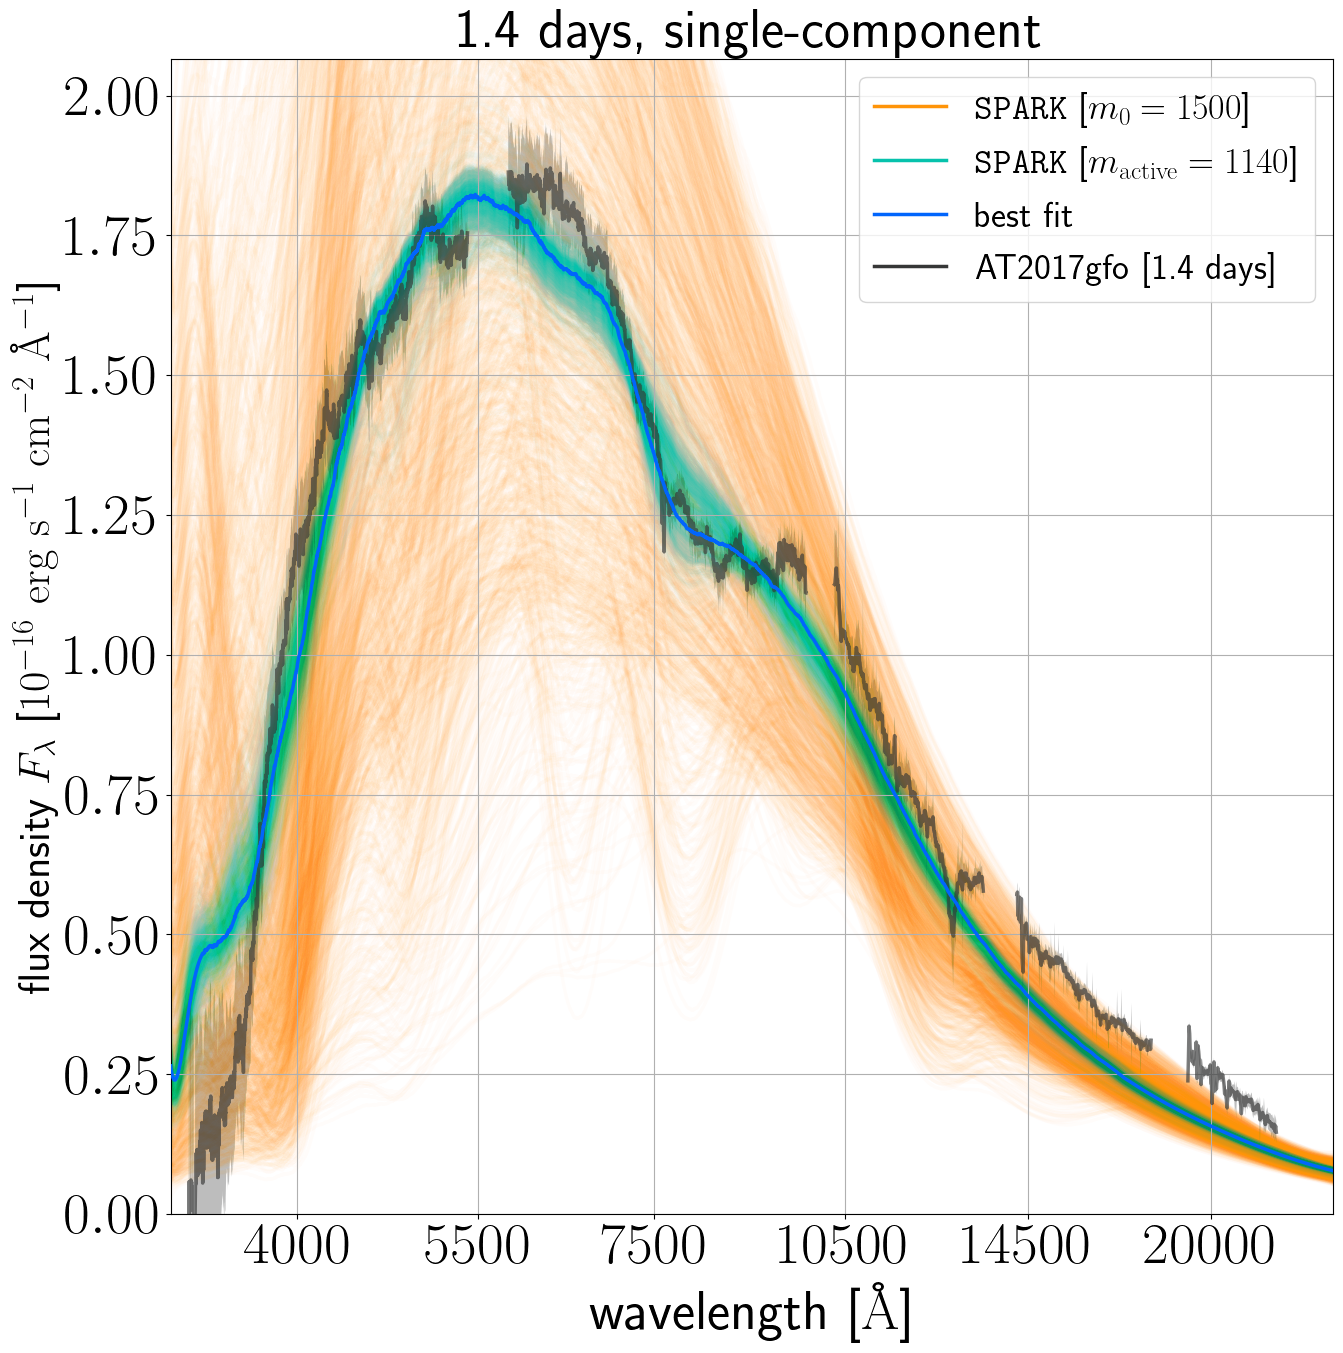
\includegraphics[width=0.47\textwidth]{figs/appendix/all-spec/220809_150113_single_all_TARDIS_evals_mactive-1140_m0-1500.png}
    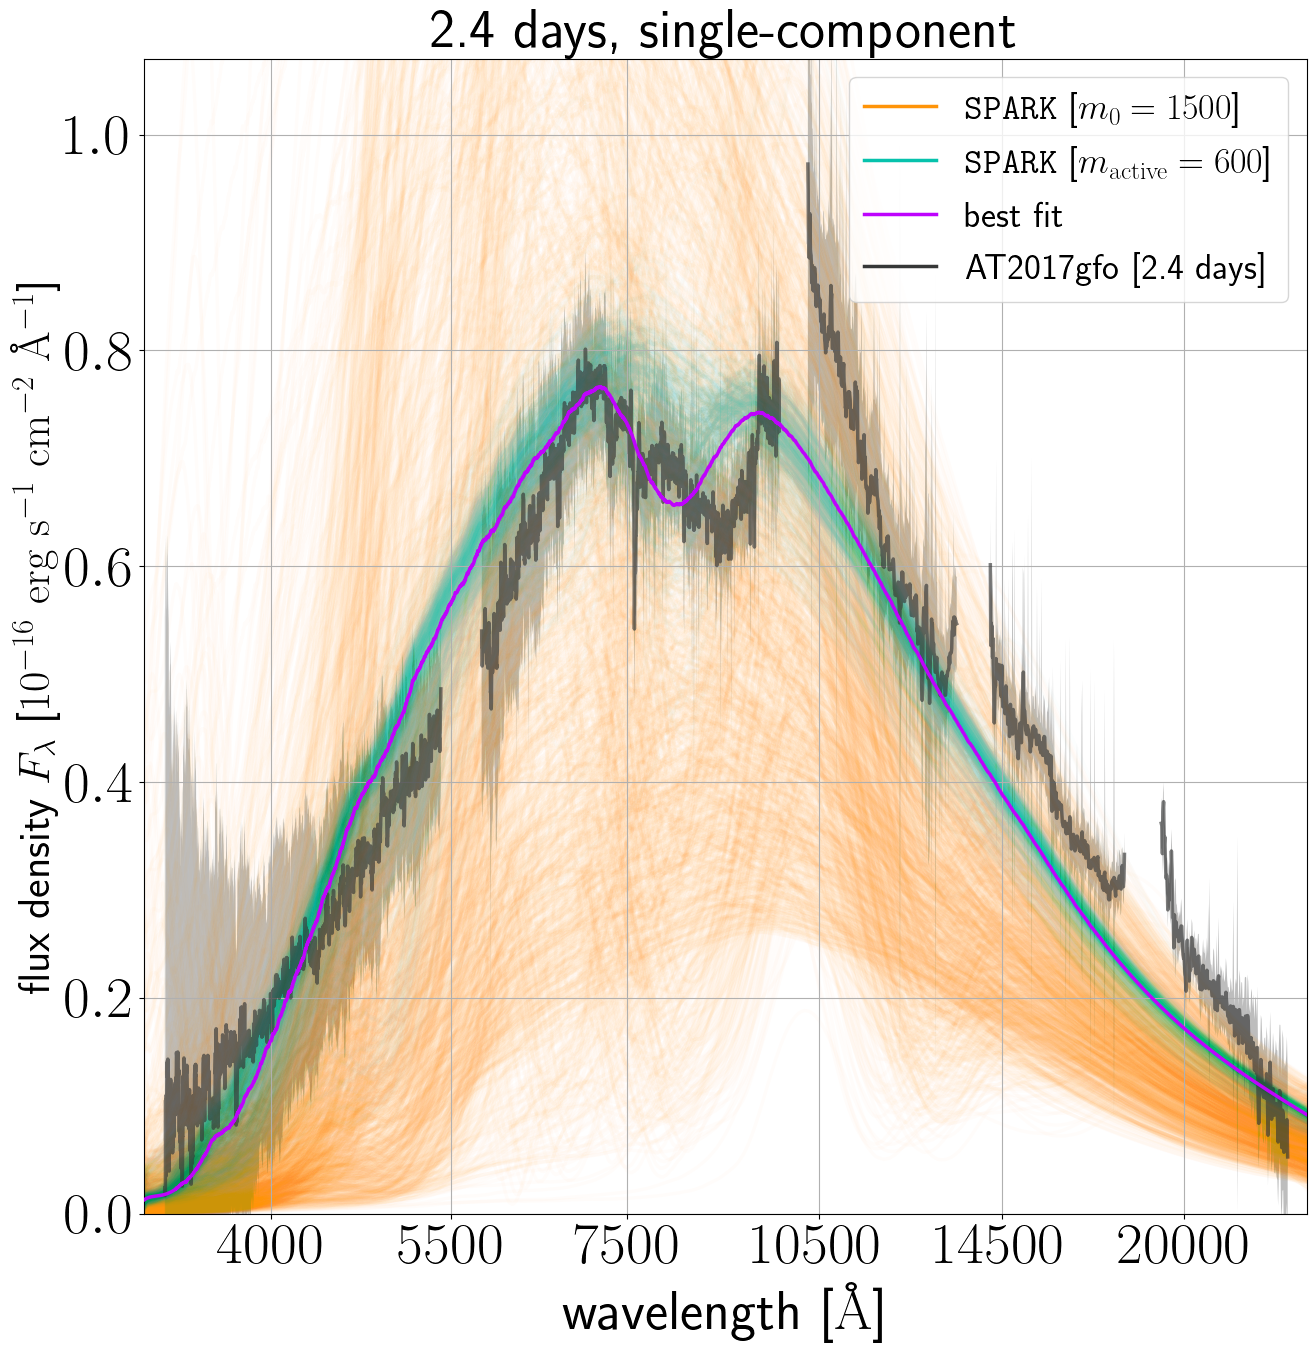
\includegraphics[width=0.47\textwidth]{figs/appendix/all-spec/221024_080947_single_all_TARDIS_evals_mactive-600_m0-1500.png}
    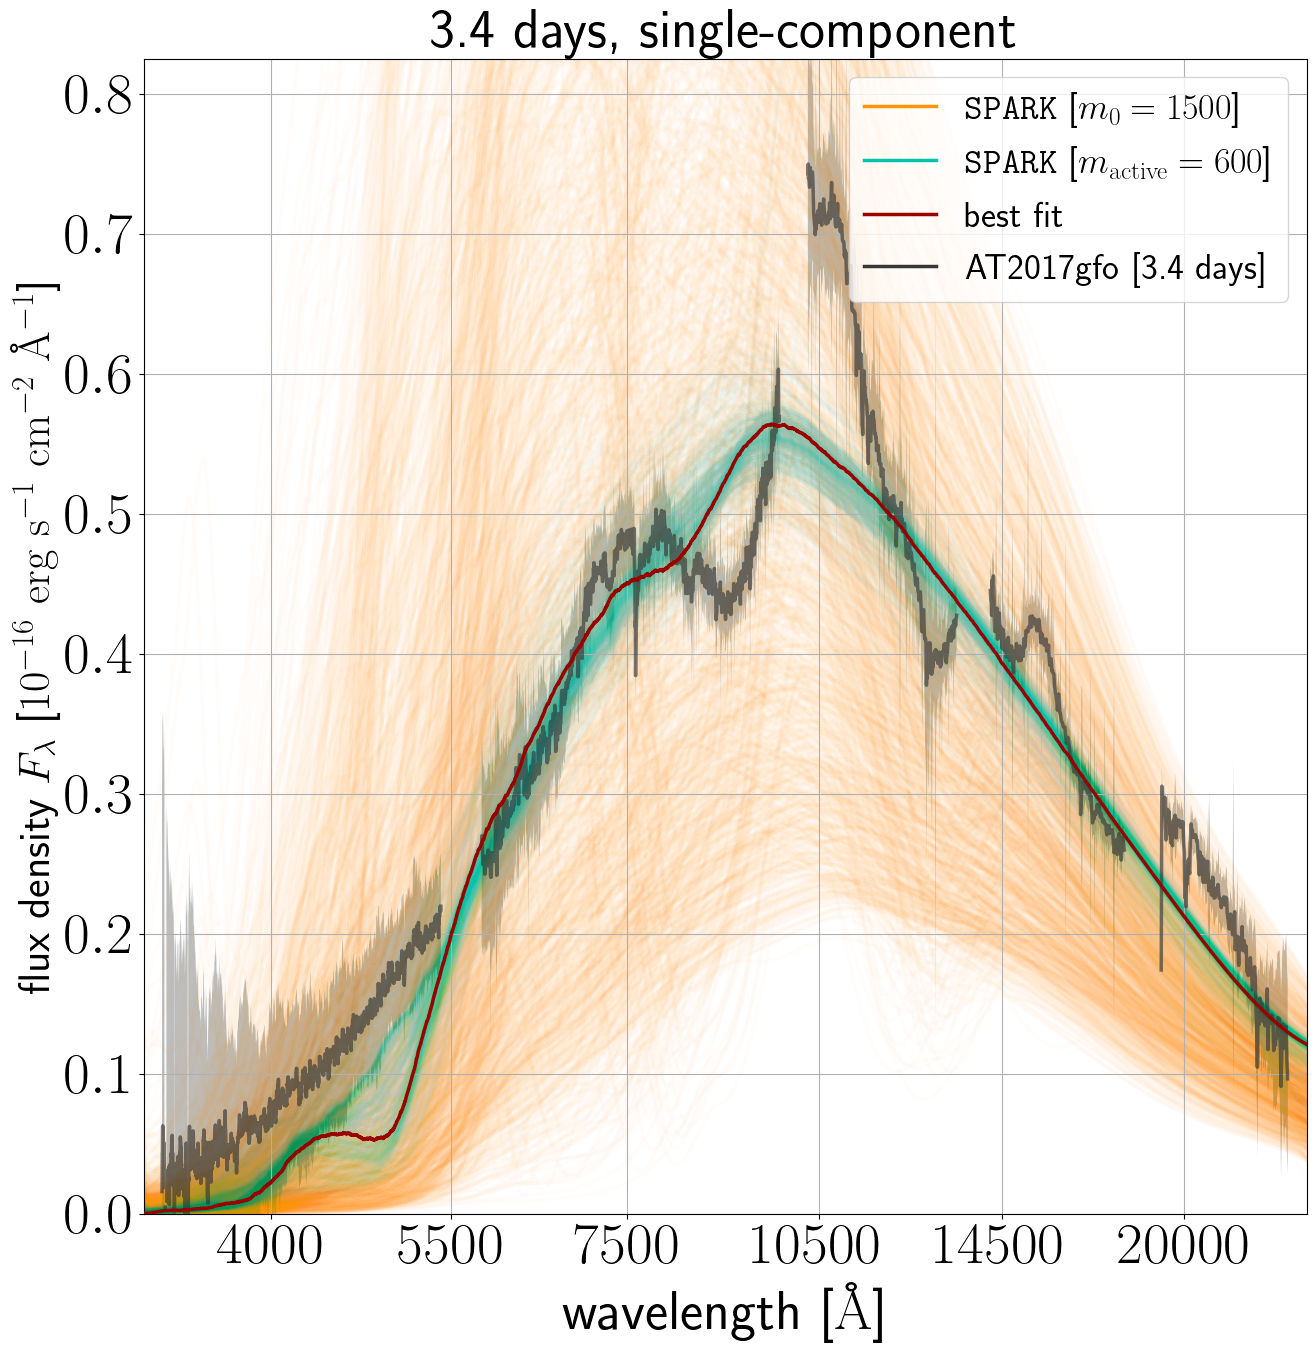
\includegraphics[width=0.47\textwidth]{figs/appendix/all-spec/230621_082134_single_all_TARDIS_evals_mactive-600_m0-1500.png}
    \figcaption{\textbf{All spectra in the training set, and the best fits, for the single-component \SPARK~runs at 2.4 and 3.4 days.} \textit{Top left:} Spectra corresponding to the $m_0 = 1500$ initial Latin Hypercube samples to explore parameter space and $m_{\mathrm{active}} = 1140$ additional active learning points selected using BAPE, for the fit to the 1.4 day spectrum of AT2017gfo, taken from V23. We also show the best fit, as obtained from the median of the posteriors. \textit{Top right:} The same, for $m_0 + m_{\mathrm{active}} = 1500 + 600$ spectra for the 2.4 day fit. \textit{Bottom center:} The same, for the 3.4 day fit. See Appendix~\ref{app:allspec_posteriors} for the complete posteriors for these single-component models. The 1.4 and 2.4 day single-component models (shown here) are favored over the multi-component models, while the 3.4 day single-component model is disfavored with respect to the multi-component model shown in Figure~\ref{fig:all_spec_multi}.}\label{fig:all_spec_single}
\end{figure*}

\begin{figure*}[!ht]
    \centering
    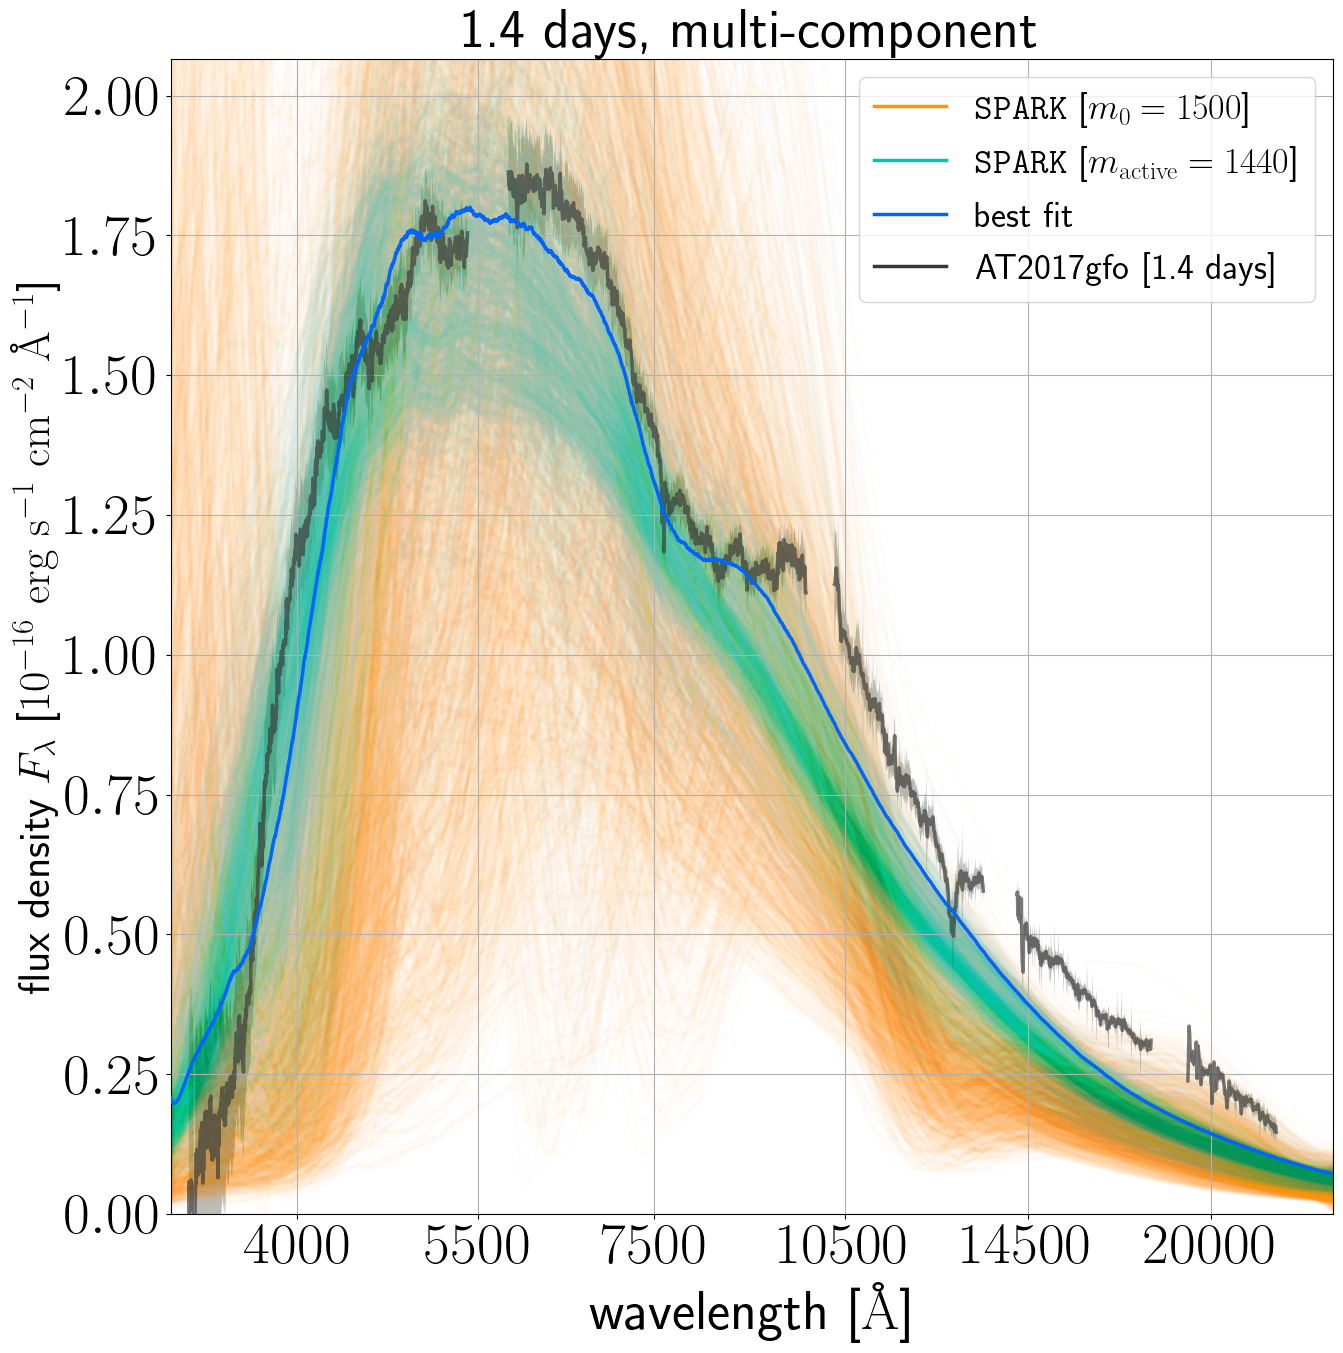
\includegraphics[width=0.47\textwidth]{figs/appendix/all-spec/230726_113032_single_all_TARDIS_evals_mactive-1440_m0-1500.png}
    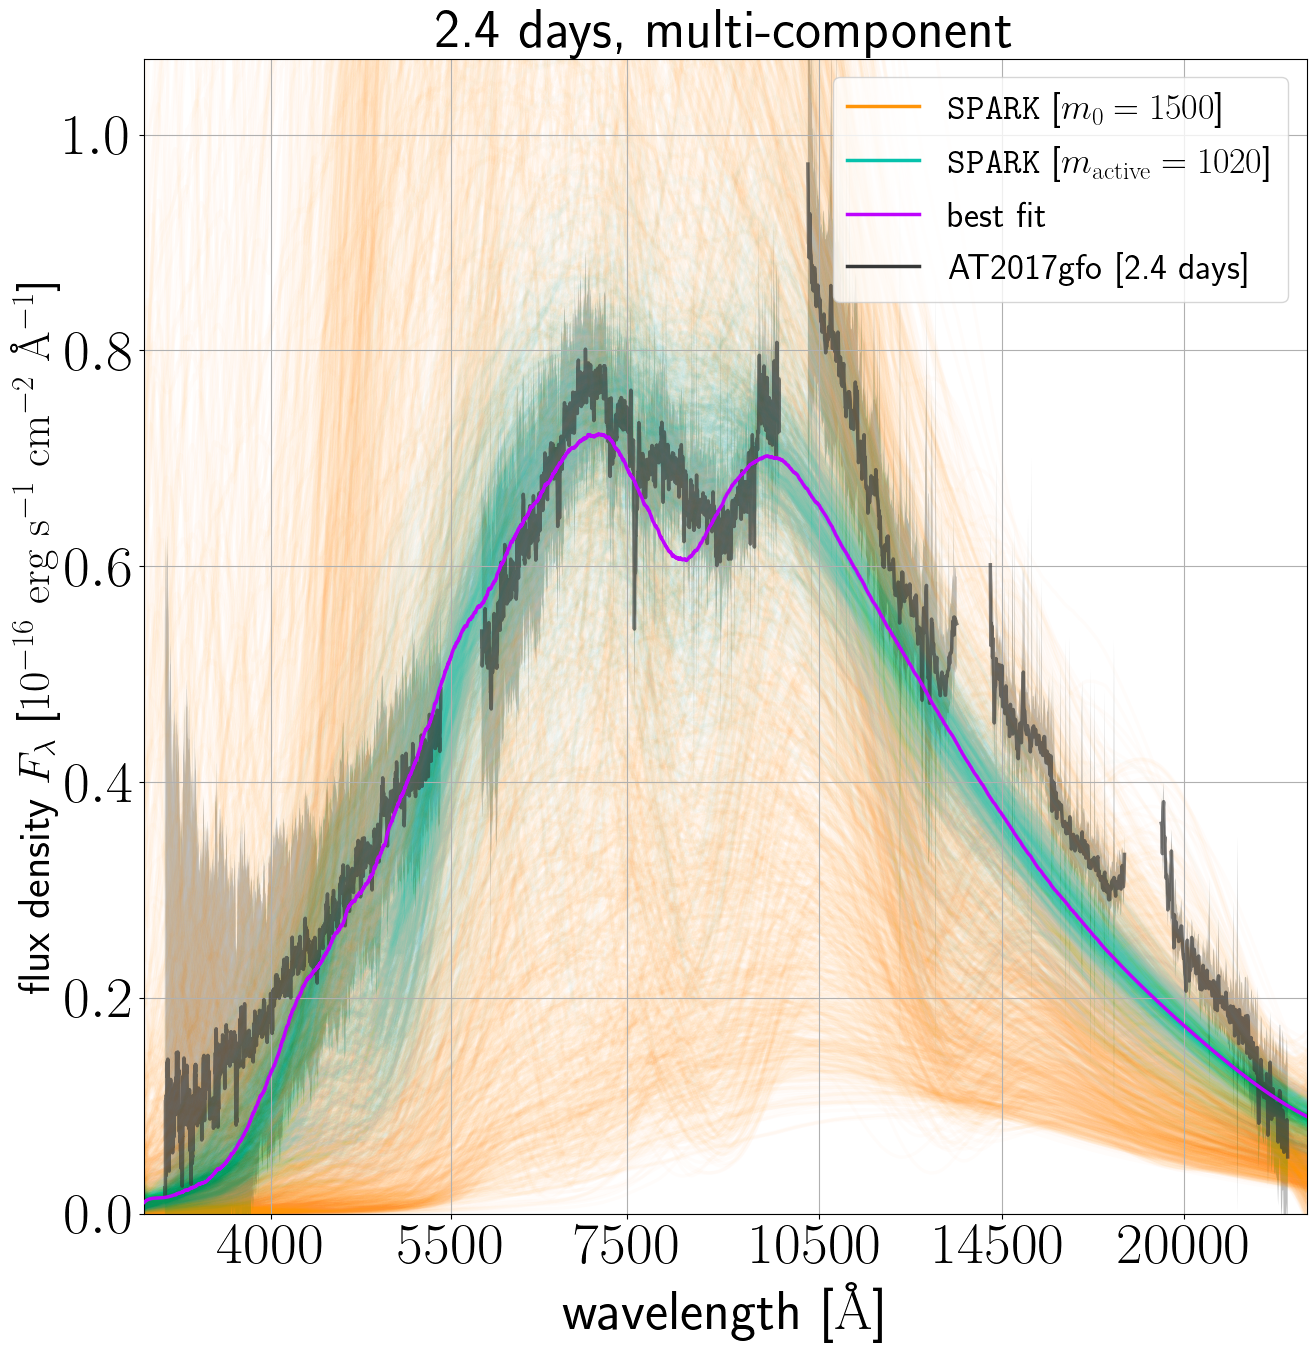
\includegraphics[width=0.47\textwidth]{figs/appendix/all-spec/230412_035244_single_all_TARDIS_evals_mactive-1020_m0-1500.png}
    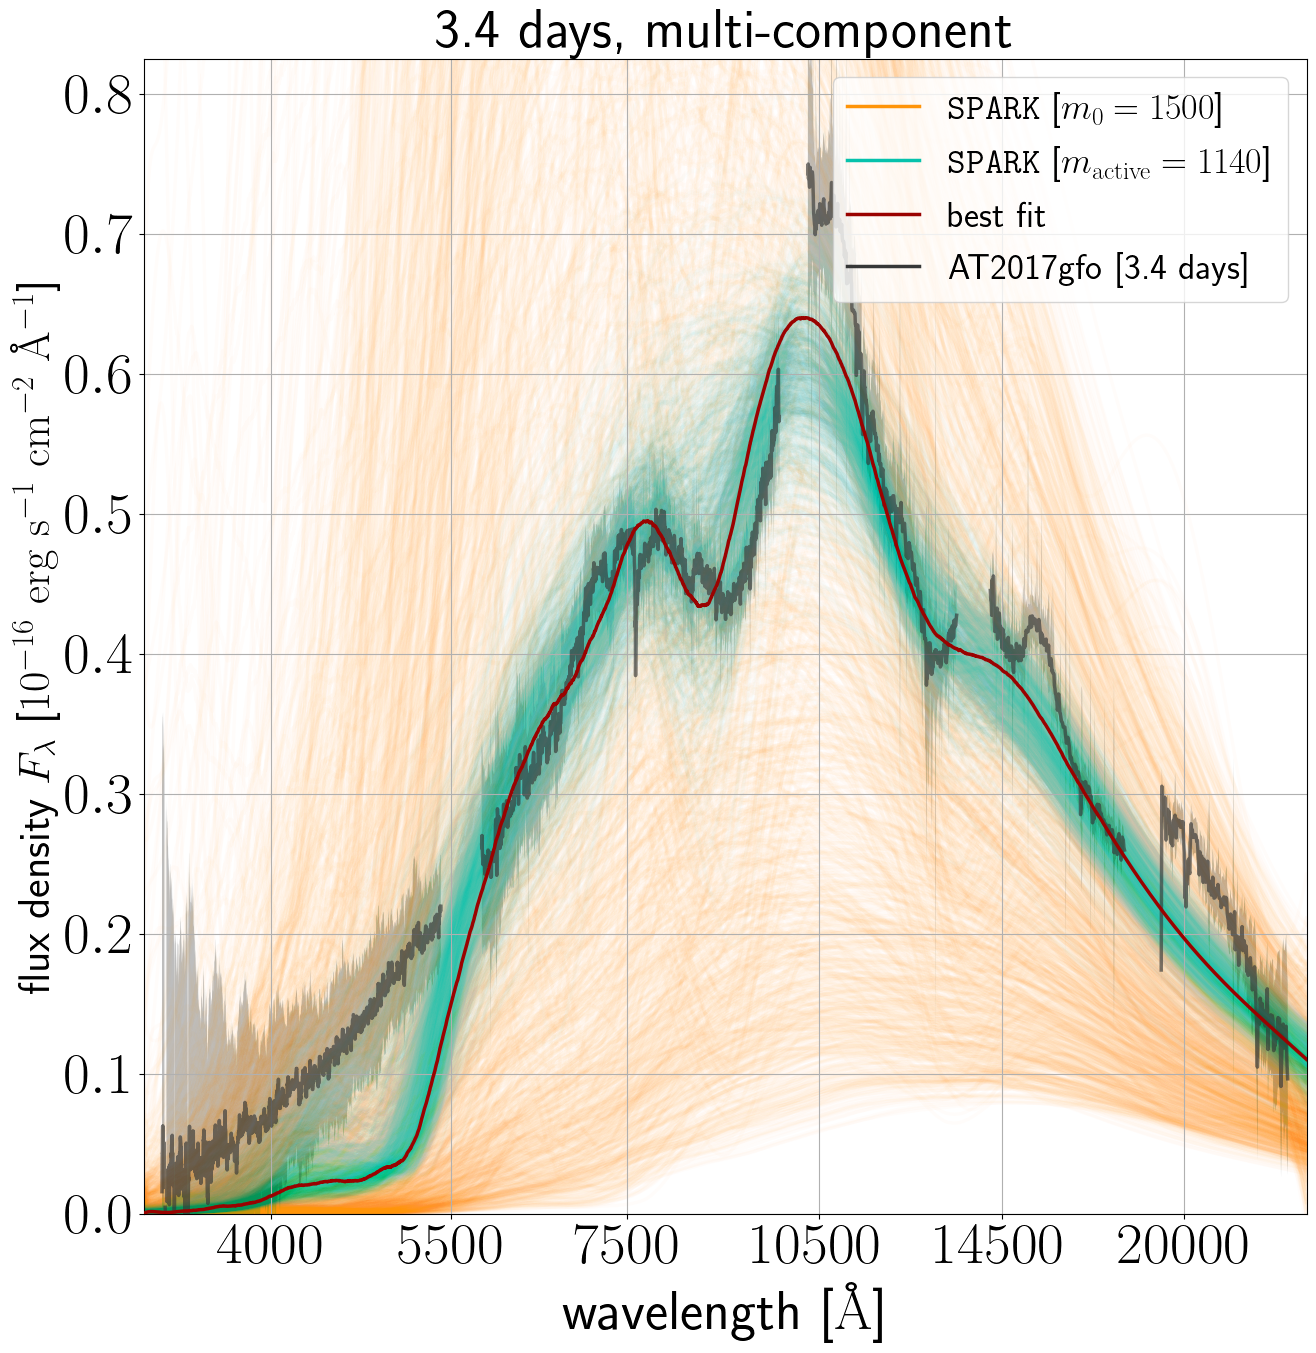
\includegraphics[width=0.47\textwidth]{figs/appendix/all-spec/230626_073230_single_all_TARDIS_evals_mactive-1140_m0-1500.png}
    \figcaption{\textbf{All spectra in the training set, and the best fits, for the multi-component \SPARK~runs at 1.4, 2.4, and 3.4 days.} \textit{Top left:} Spectra corresponding to the $m_0 = 1500$ initial Latin Hypercube samples to explore parameter space and $m_{\mathrm{active}} = 1440$ additional active learning points selected using BAPE, for the fit to the 1.4 day spectrum of AT2017gfo. We also show the best fit, as obtained from the median of the posteriors. \textit{Top right:} The same, for the 2.4 day fit, where $m_{\mathrm{active}} = 1020$ active learning samples are required. \textit{Bottom center:} The same for the 3.4 day fit, where $m_{\mathrm{active}} = 1140$ active learning samples are required. See Appendix~\ref{app:allspec_posteriors} for the complete posteriors for these multi-component models. The 1.4 and 2.4 day multi-component models shown here are disfavored with respect to the single-component models; the 3.4 day multi-component model shown here is favored over the single-component.}\label{fig:all_spec_multi}
\end{figure*}




\begin{figure*}[!ht]
    \includegraphics[width=0.95\textwidth]{figs/appendix/corners/221022_084052_dynesty_corner_pretty_smooth2d0.05_nodatapts.png}
    \figcaption{\textbf{Posterior from the single-component \SPARK~run at 2.4 days.} All posteriors are obtained through dynamic nested sampling of the surrogate Gaussian Process using \texttt{dynesty} (\citealt{speagle20}). The posterior presents some bimodality, most evident in the $s/k_{\mathrm{B}}$ dimension. In Figure~\ref{fig:corner_single_2.4_zoom}, we discard samples with $s/k_{\mathrm{B}} \geqslant 25.0$. This lower-entropy mode of the posterior is our preferred model.}\label{fig:corner_single_2.4}
\end{figure*}

\begin{figure*}[!ht]
    \includegraphics[width=0.95\textwidth]{figs/appendix/corners/221022_084052_dynesty_corner_pretty_smooth2d0.05_nodatapts_zoom.png}
    \figcaption{\textbf{Posterior from the single-component \SPARK~run at 2.4 days, zoomed in to the mode which produces the best fit.} Samples $s/k_{\mathrm{B}} \geqslant 25.0$ are discarded to show only this mode of the posterior, which corresponds to the preferred model in Table~\ref{tab:bestfit_single}.}\label{fig:corner_single_2.4_zoom}
\end{figure*}

\begin{figure*}[!ht]
    \includegraphics[width=0.95\textwidth]{figs/appendix/corners/230618_143307_dynesty_corner_pretty_mactive-600_smooth2d0.05_nodatapts.png}
    \figcaption{\textbf{Posterior from the single-component \SPARK~run at 3.4 days.} The posterior at this epoch is highly multi-modal, as most evident in the $\rho_0,~Y_{\mathrm{e}},~\mathrm{and}~s/k_{\mathrm{B}}$ dimensions. Although none of these modes in the posterior correspond to a good fit, and the multi-component model is favored at 3.4 days, we find the higher-$\rho_0$, mid-$Y_{\mathrm{e}}$, low-$s$ mode produces the best possible fit with single-component ejecta. In Figure~\ref{fig:corner_single_3.4_zoom}, we highlight this mode of the posterior by discarding samples outside the range $\log_{10}(\rho_0 / \mathrm{g~cm^{-3}}) \in [-15.0, -14.0] \cup Y_{\mathrm{e}} \in [0.13, 0.29] \cup s/k_{\mathrm{B}} \in [10.0, 25.0]$.  }\label{fig:corner_single_3.4}
\end{figure*}

\begin{figure*}[!ht]
    \includegraphics[width=0.95\textwidth]{figs/appendix/corners/230618_143307_dynesty_corner_pretty_mactive-600_smooth2d0.05_nodatapts_zoom-midYe-lows-highdens_add-nlive-30000.png}
    \figcaption{\textbf{Posterior from the single-component \SPARK~run at 3.4 days, zoomed in to the mode which produces the best fit.} Samples outside the range $\log_{10}(\rho_0 / \mathrm{g~cm^{-3}}) \in [-15.0, -14.0] \cup Y_{\mathrm{e}} \in [0.13, 0.29] \cup s/k_{\mathrm{B}} \in [10.0, 25.0]$ are discarded to show only the mode of the posterior which corresponds to the preferred model in Table~\ref{tab:bestfit_single}.}\label{fig:corner_single_3.4_zoom}
\end{figure*}

\begin{figure*}[!ht]
    \includegraphics[width=0.95\textwidth]{figs/appendix/corners/230103_064024_dynesty_corner_pretty_mactive-1440_smooth2d0.05_nodatapts_overridetitles.png}
    \figcaption{\textbf{Posterior from the multi-component \SPARK~run at 1.4 days.}}\label{fig:corner_multi_1.4}
\end{figure*}

\begin{figure*}[!ht]
    \includegraphics[width=0.95\textwidth]{figs/appendix/corners/230103_060017_dynesty_corner_pretty_mactive-1020_smooth2d0.05_nodatapts_overridetitles.png}
    \figcaption{\textbf{Posterior from the multi-component \SPARK~run at 2.4 days.} The posterior contains one lower-probability mode, most evident in the $v_{\mathrm{inner},1}$ dimension. We ignore this mode, as the median of the higher-probability mode yields our best fit, as given in Table~\ref{tab:bestfit_multi}.}\label{fig:corner_multi_2.4}
\end{figure*}

\begin{figure*}[!ht]
    \includegraphics[width=0.95\textwidth]{figs/appendix/corners/230622_230103_dynesty_corner_pretty_mactive-1140_smooth2d0.05_nodatapts_overridetitles.png}
    \figcaption{\textbf{Posterior from the multi-component \SPARK~run at 3.4 days.} As at 2.4 days, the posterior contains one lower-probability mode, most evident in the $v_{\mathrm{inner},1}$ dimension. We once again ignore this mode, as the median of the higher-probability mode yields our best fit, as given in Table~\ref{tab:bestfit_multi}.}\label{fig:corner_multi_3.4}
\end{figure*}





%%% === APPENDIX B === %%%
%% COMPARE ABUNDANCES OF COMPONENTS %%
\section{Comparison of multi-component abundances}\label{app:compare_components}

\begin{figure*}[!ht]
    \centering
    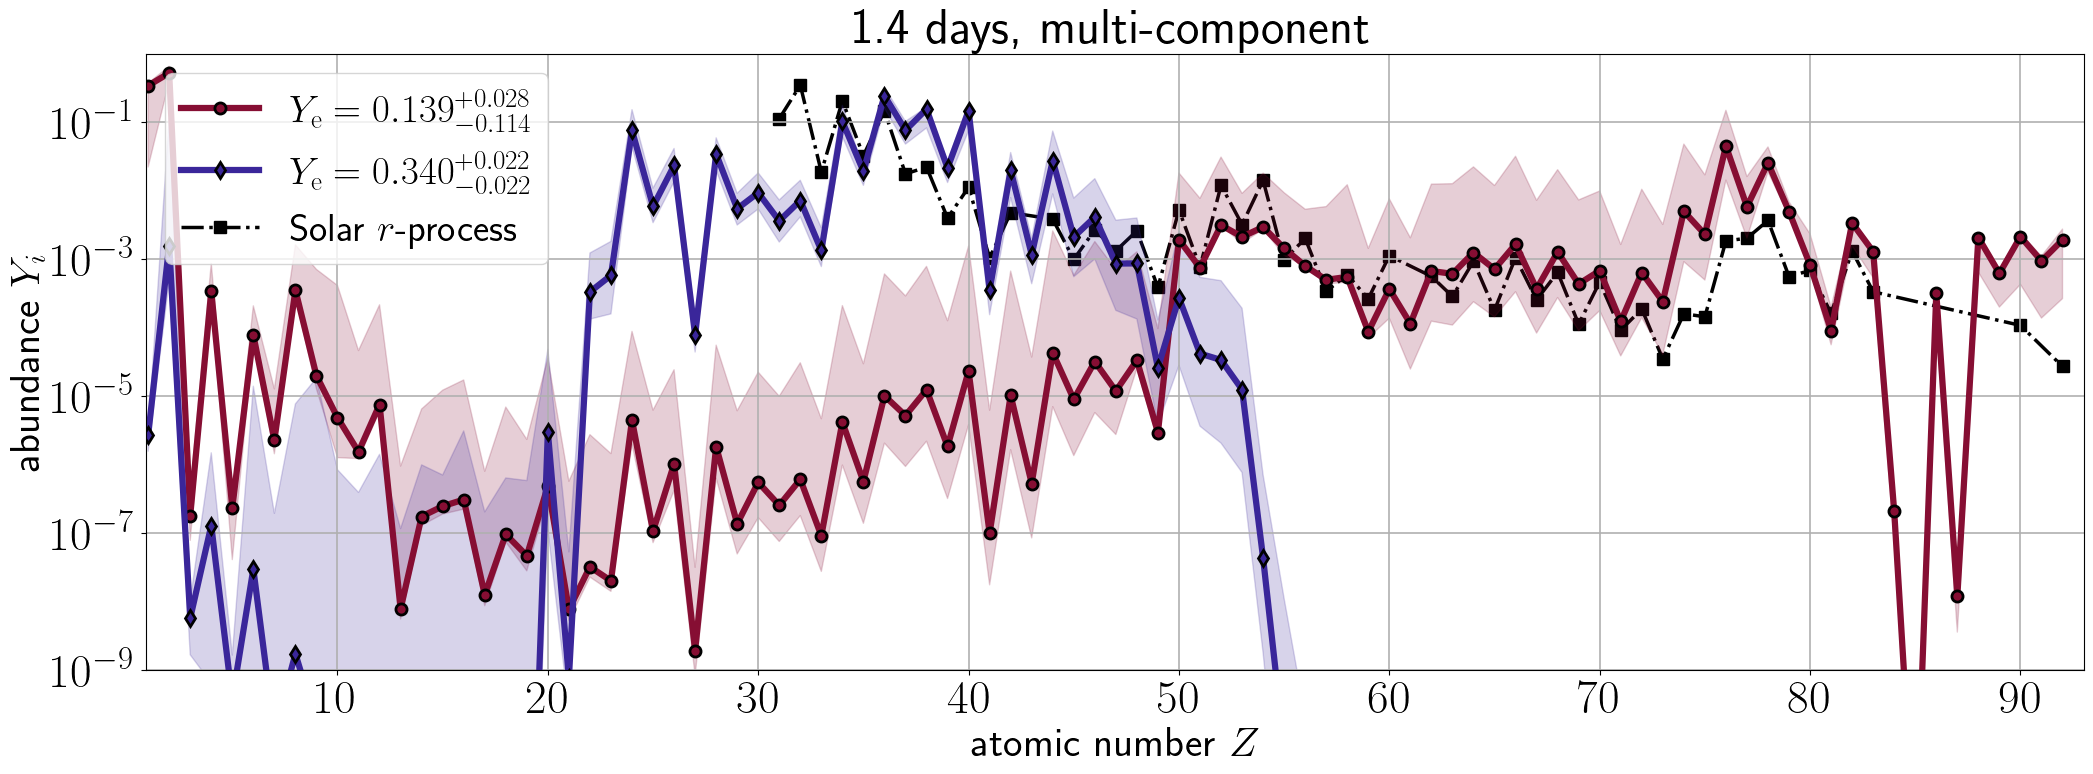
\includegraphics[width=0.98\textwidth]{figs/appendix/compare-components/compare_abunds_230103_064024_components_dynesty_100samples.png}
    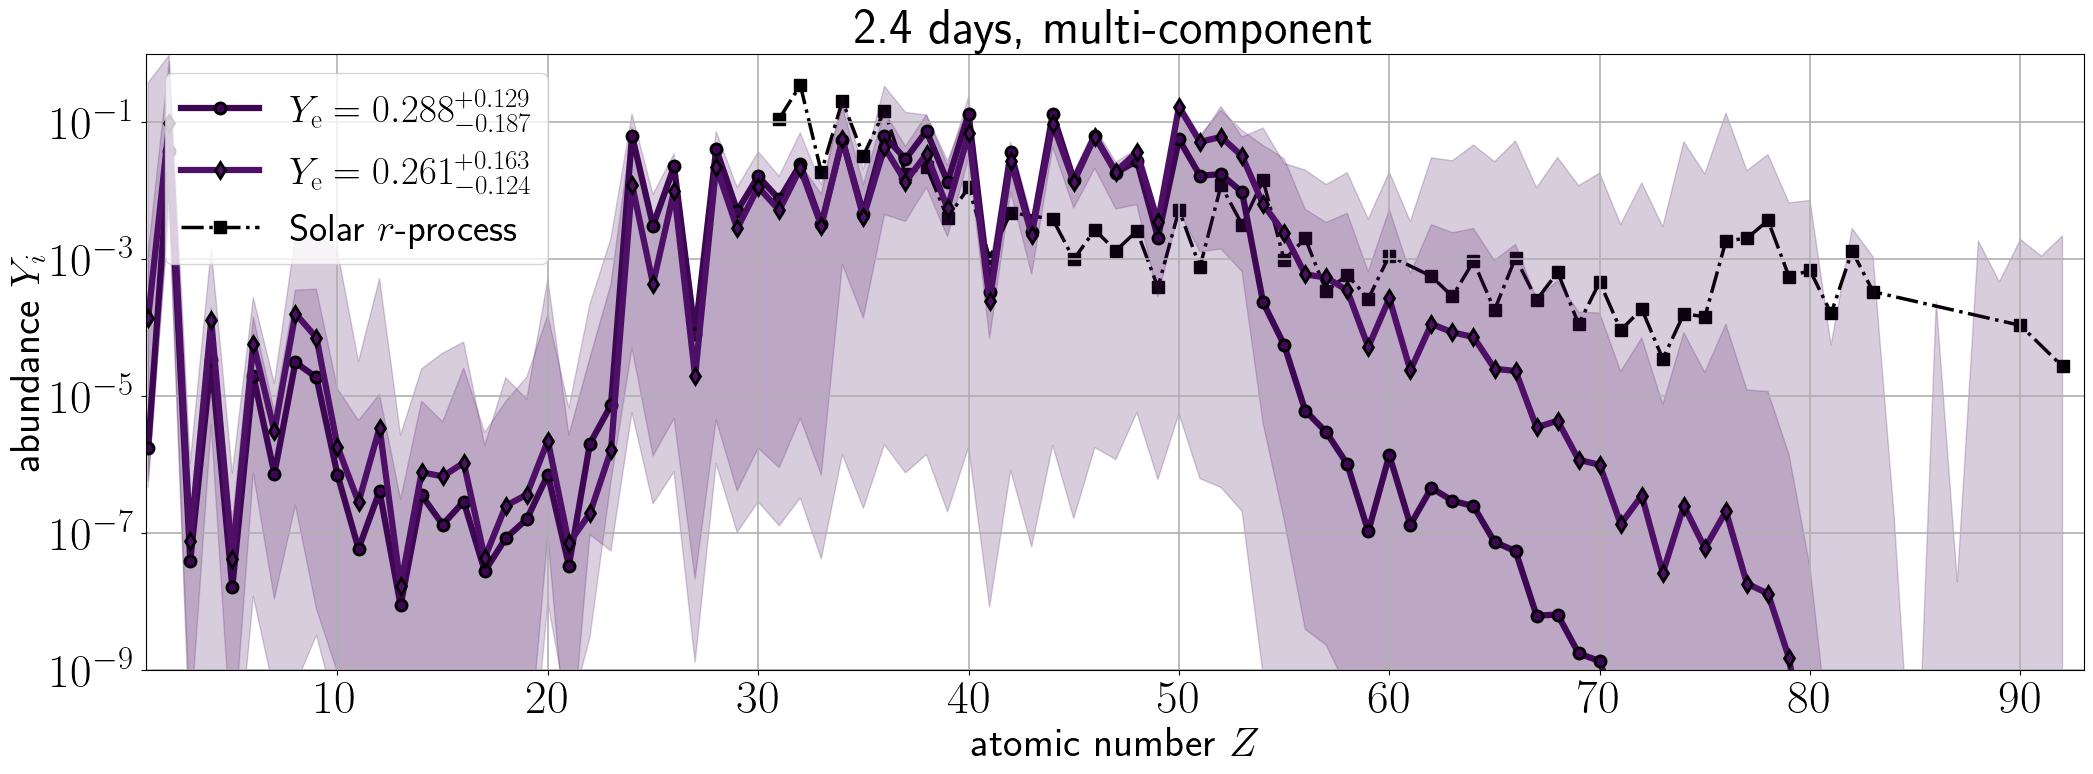
\includegraphics[width=0.98\textwidth]{figs/appendix/compare-components/compare_abunds_230103_060017_components_dynesty_100samples.png}
    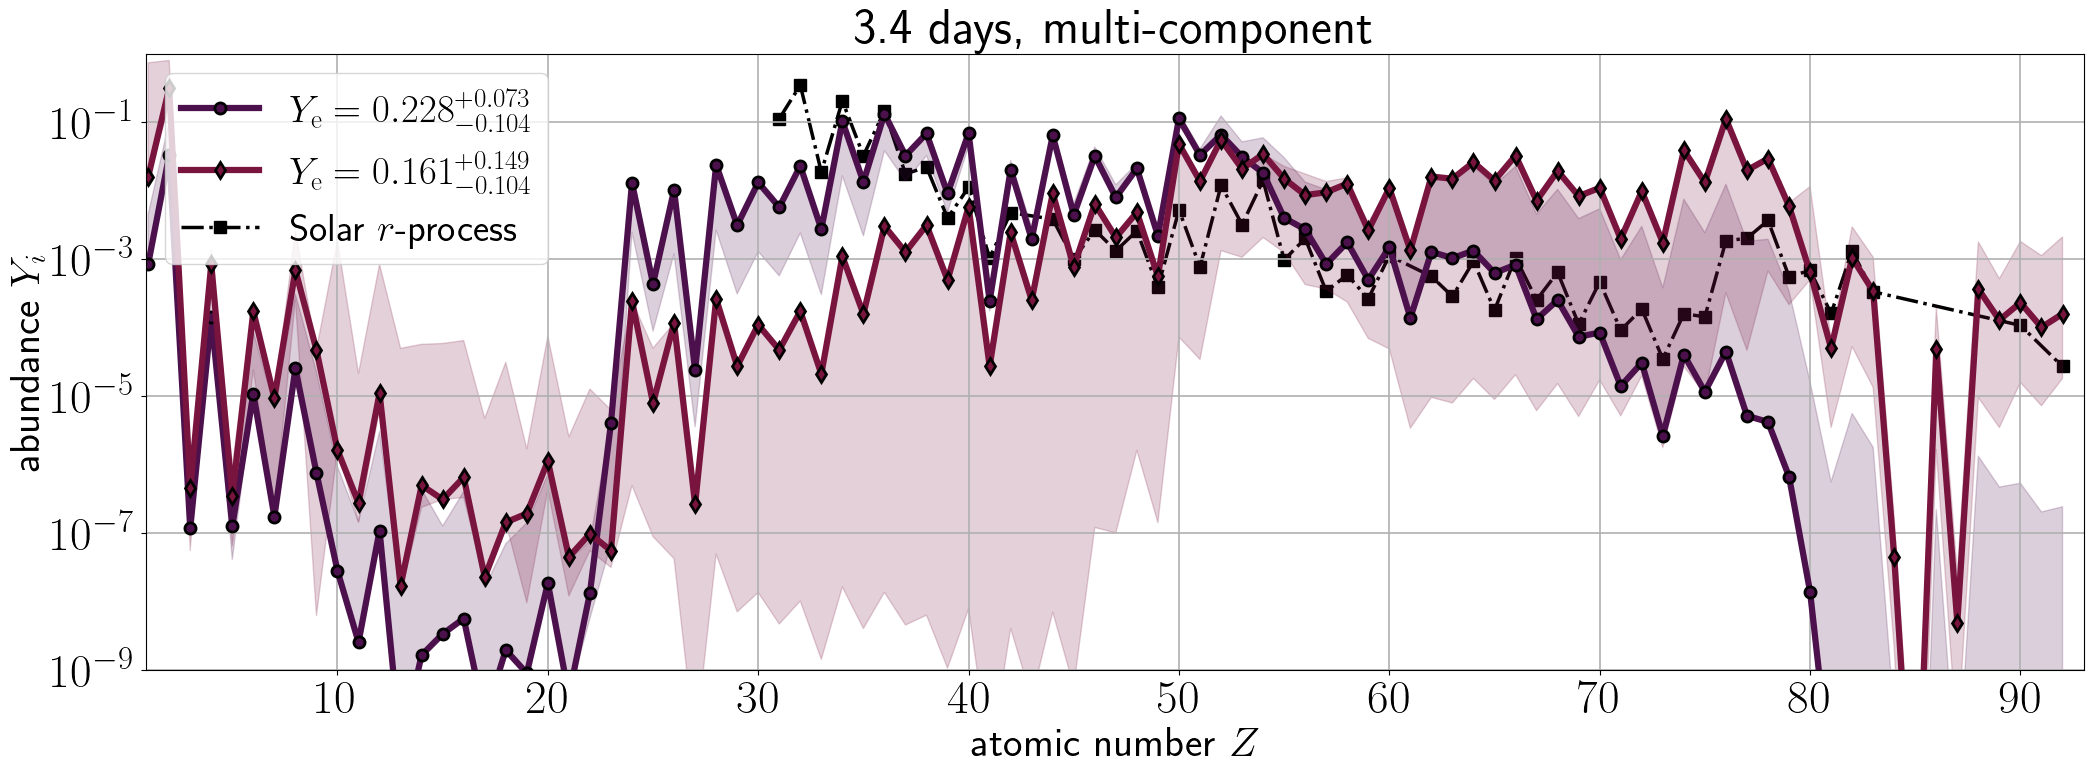
\includegraphics[width=0.98\textwidth]{figs/appendix/compare-components/compare_abunds_230622_230103_components_dynesty_100samples.png}
    \figcaption{\textbf{Comparison of the abundances of different components for the multi-component models at 1.4, 2.4, and 3.4 days.} The abundance patterns for the two components are similar at 2.4 days. At 3.4 days, there is a redder (lower-$Y_e$) component with more lanthanides and a relative dearth of the crucial element strontium (${}_{38}$Sr), while the bluer (higher-$Y_e$) component contains $\sim$10$\times$ as much Sr and a dearth of lanthanides. Importantly, these plots show abundances, and not mass fractions: the components are approximately equipartitioned in mass at 2.4 and 3.4 days, such that both contribute to the emergent spectrum, while the redder component at 1.4 days has $\sim$100$\times$ less mass than the blue and thus its contribution to the emergent spectrum is negligible, despite having a substantially different abundance pattern.}\label{fig:abunds_components_compare}
\end{figure*}

Figure~\ref{fig:abunds_components_compare} compares the abundances of each component in the multi-component models at 1.4, 2.4, and 3.4 days. Crucially, these are abundances, not mass fractions: while the components are approximately equipartitioned in mass at 2.4 and 3.4 days, at 1.4 days, the bluer has $\sim$100$\times$ the mass of the redder, and the redder has negligible impact on the emergent spectrum, despite having a substantially different abundance pattern.



% %%% === APPENDIX C === %%%
% %% LEAVE-ONE-OUT SPECTRA %%
% \section{Leave-one-out Spectra---Non-Preferred Models}\label{app:leave_out_nonpref}

% In Figure~\ref{fig:leave_out_nonpref}, we show leave-one-out spectra for the non-preferred fits: multi-component for 1.4 and 2.4 days, and single-component for 3.4 days.

% \begin{figure*}[!ht]
%     \centering
%     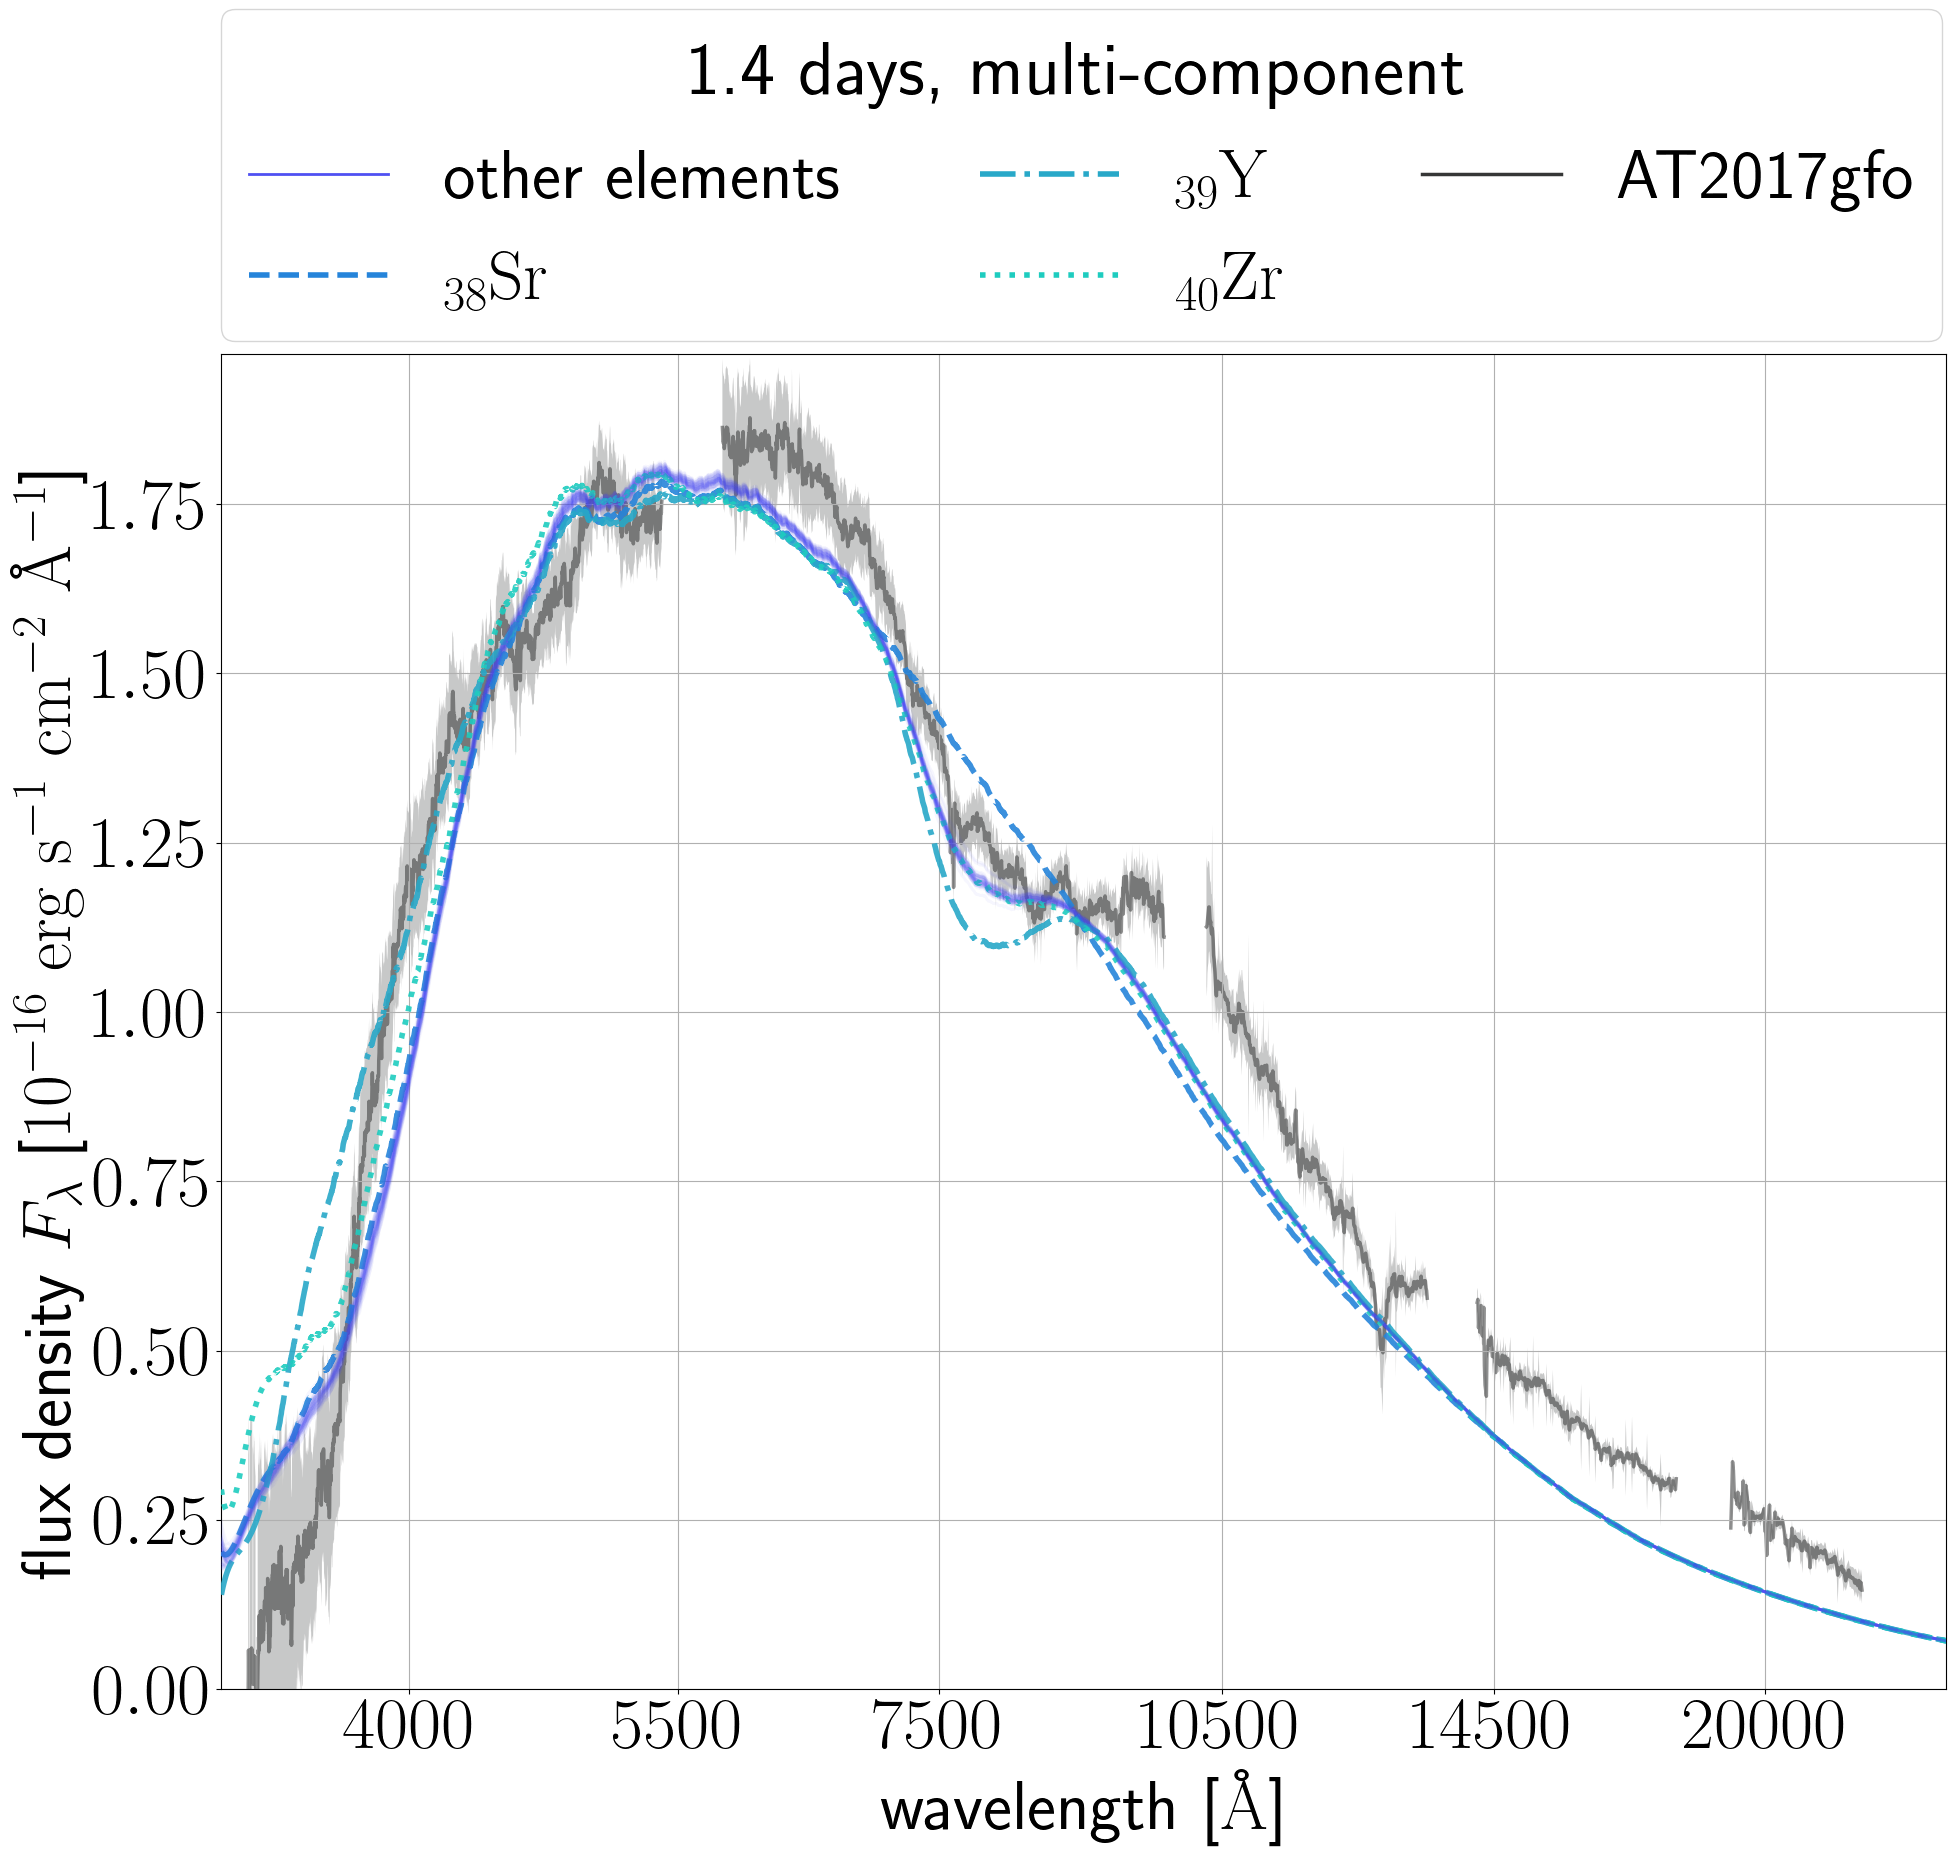
\includegraphics[width=0.47\textwidth]{figs/appendix/LoO/230729_020047_leaveoneout_all_TARDIS_evals_label-interest-38-39-40.png}
%     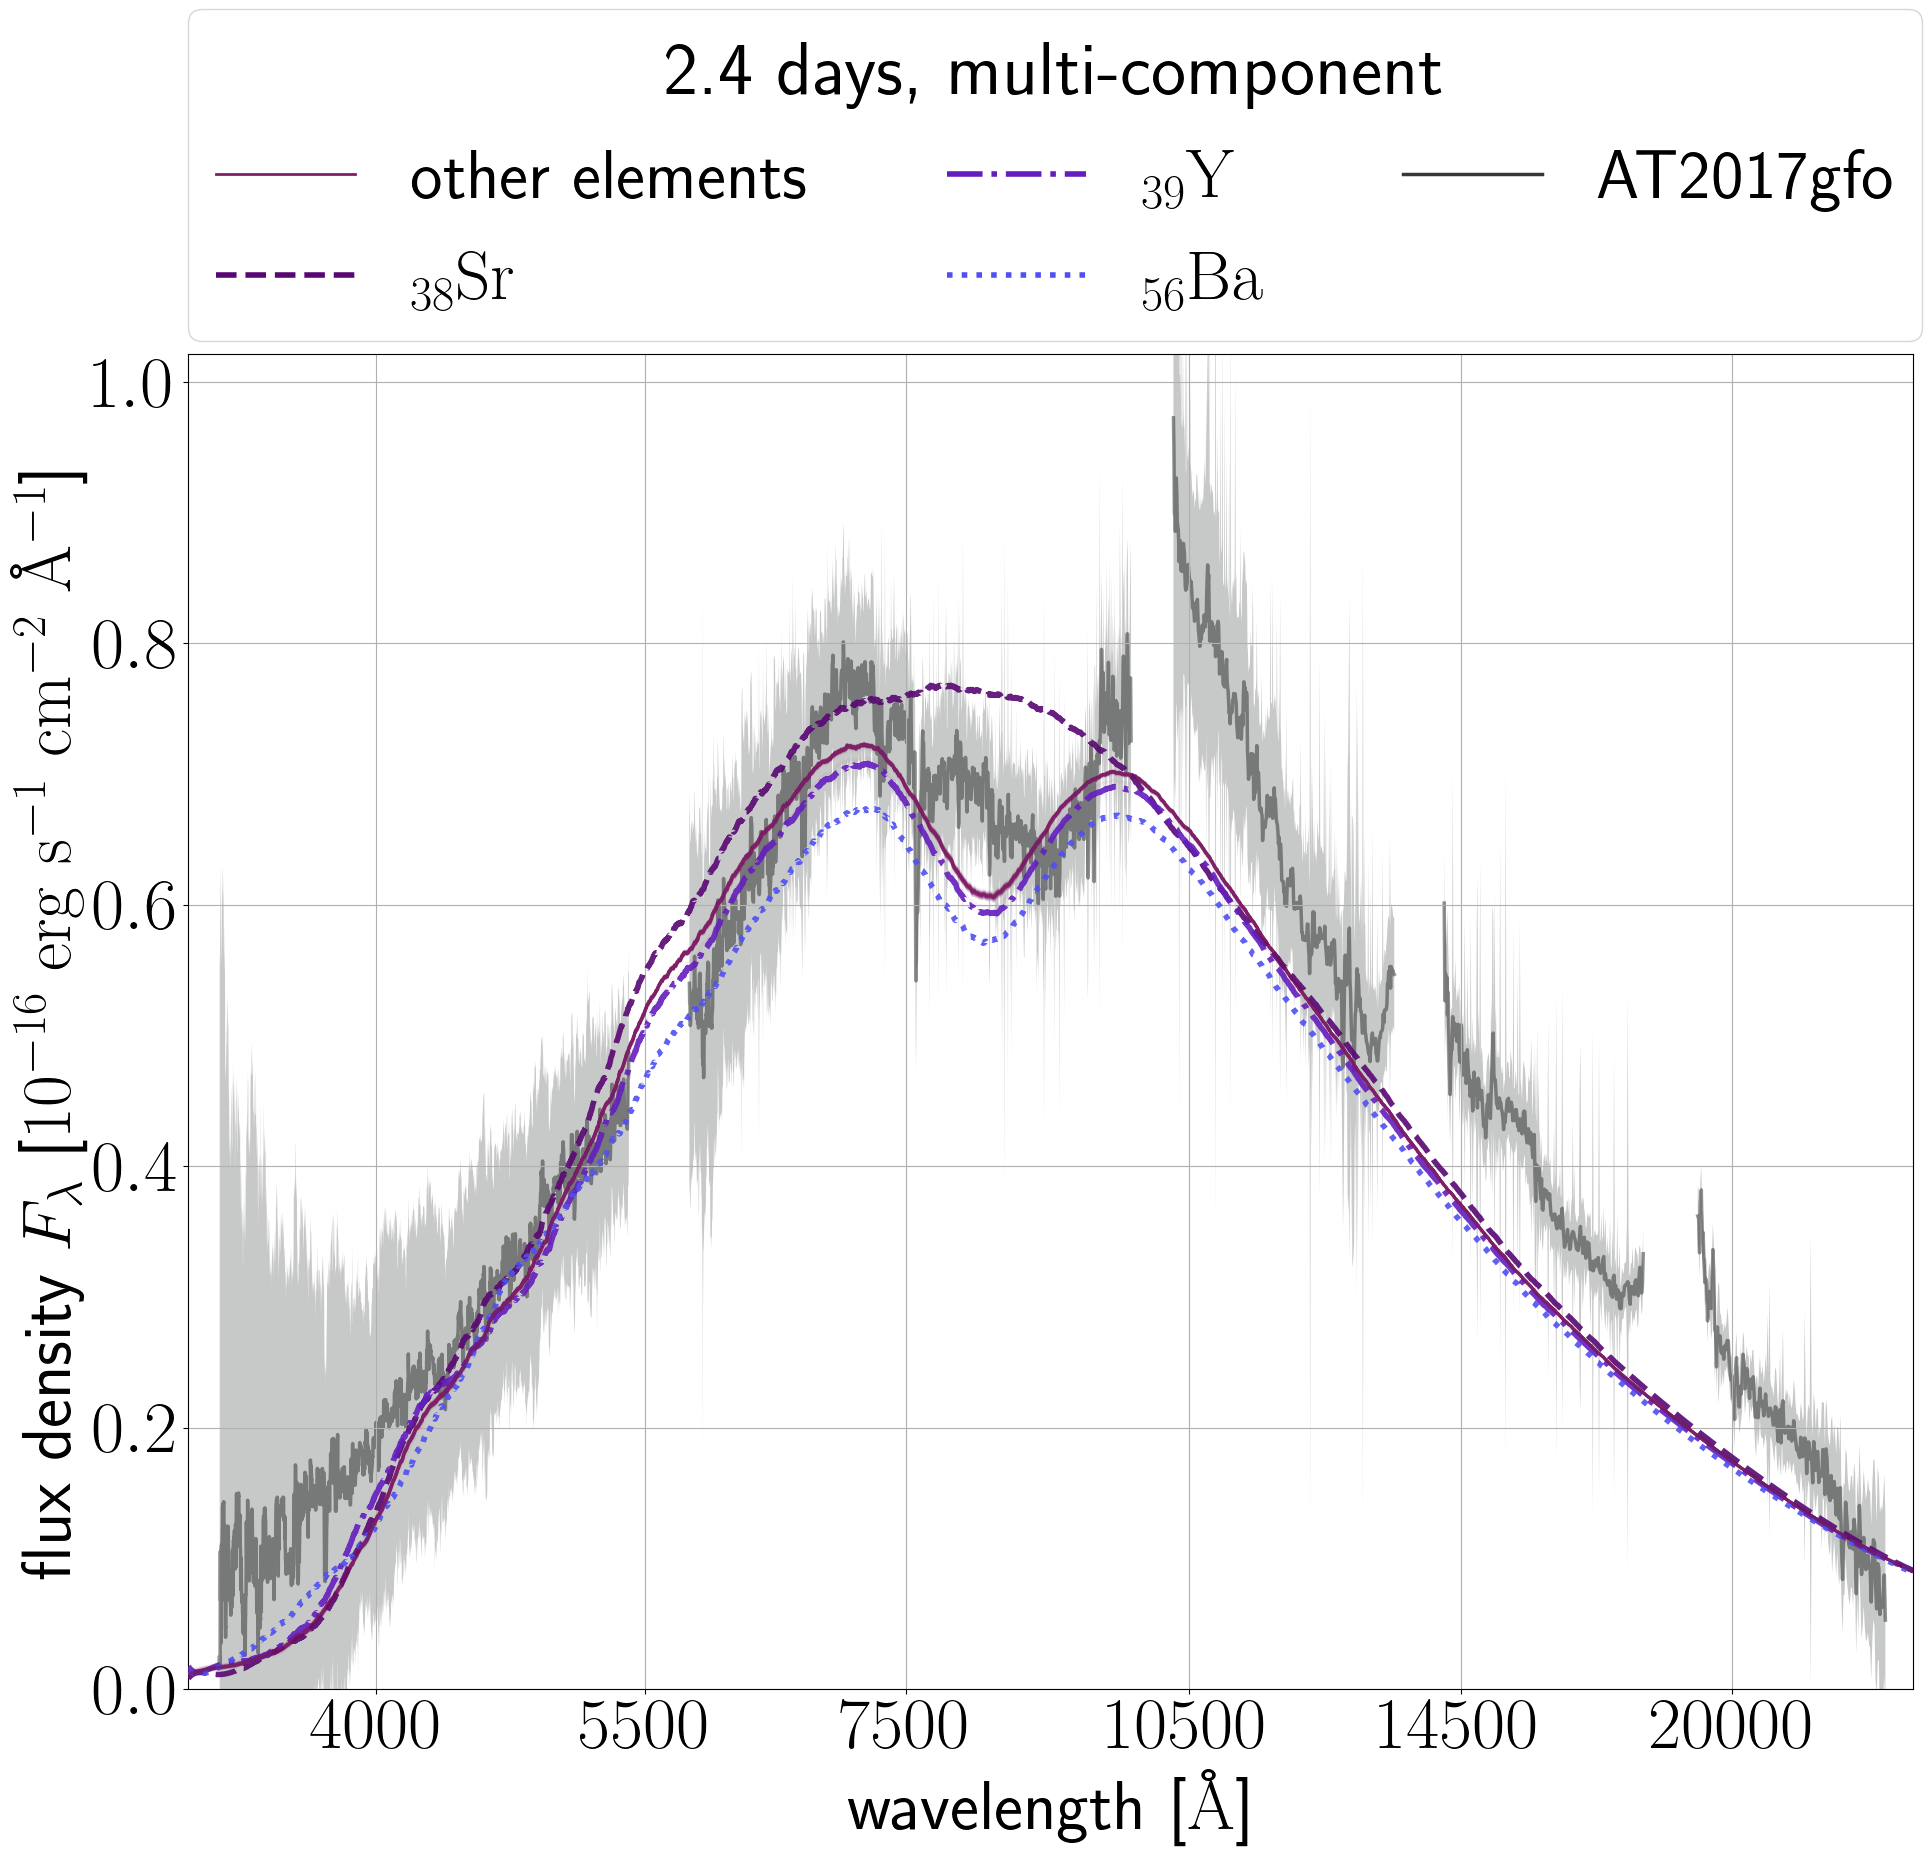
\includegraphics[width=0.47\textwidth]{figs/appendix/LoO/230504_003423_leaveoneout_all_TARDIS_evals_label-interest-38-39-56.png}
%     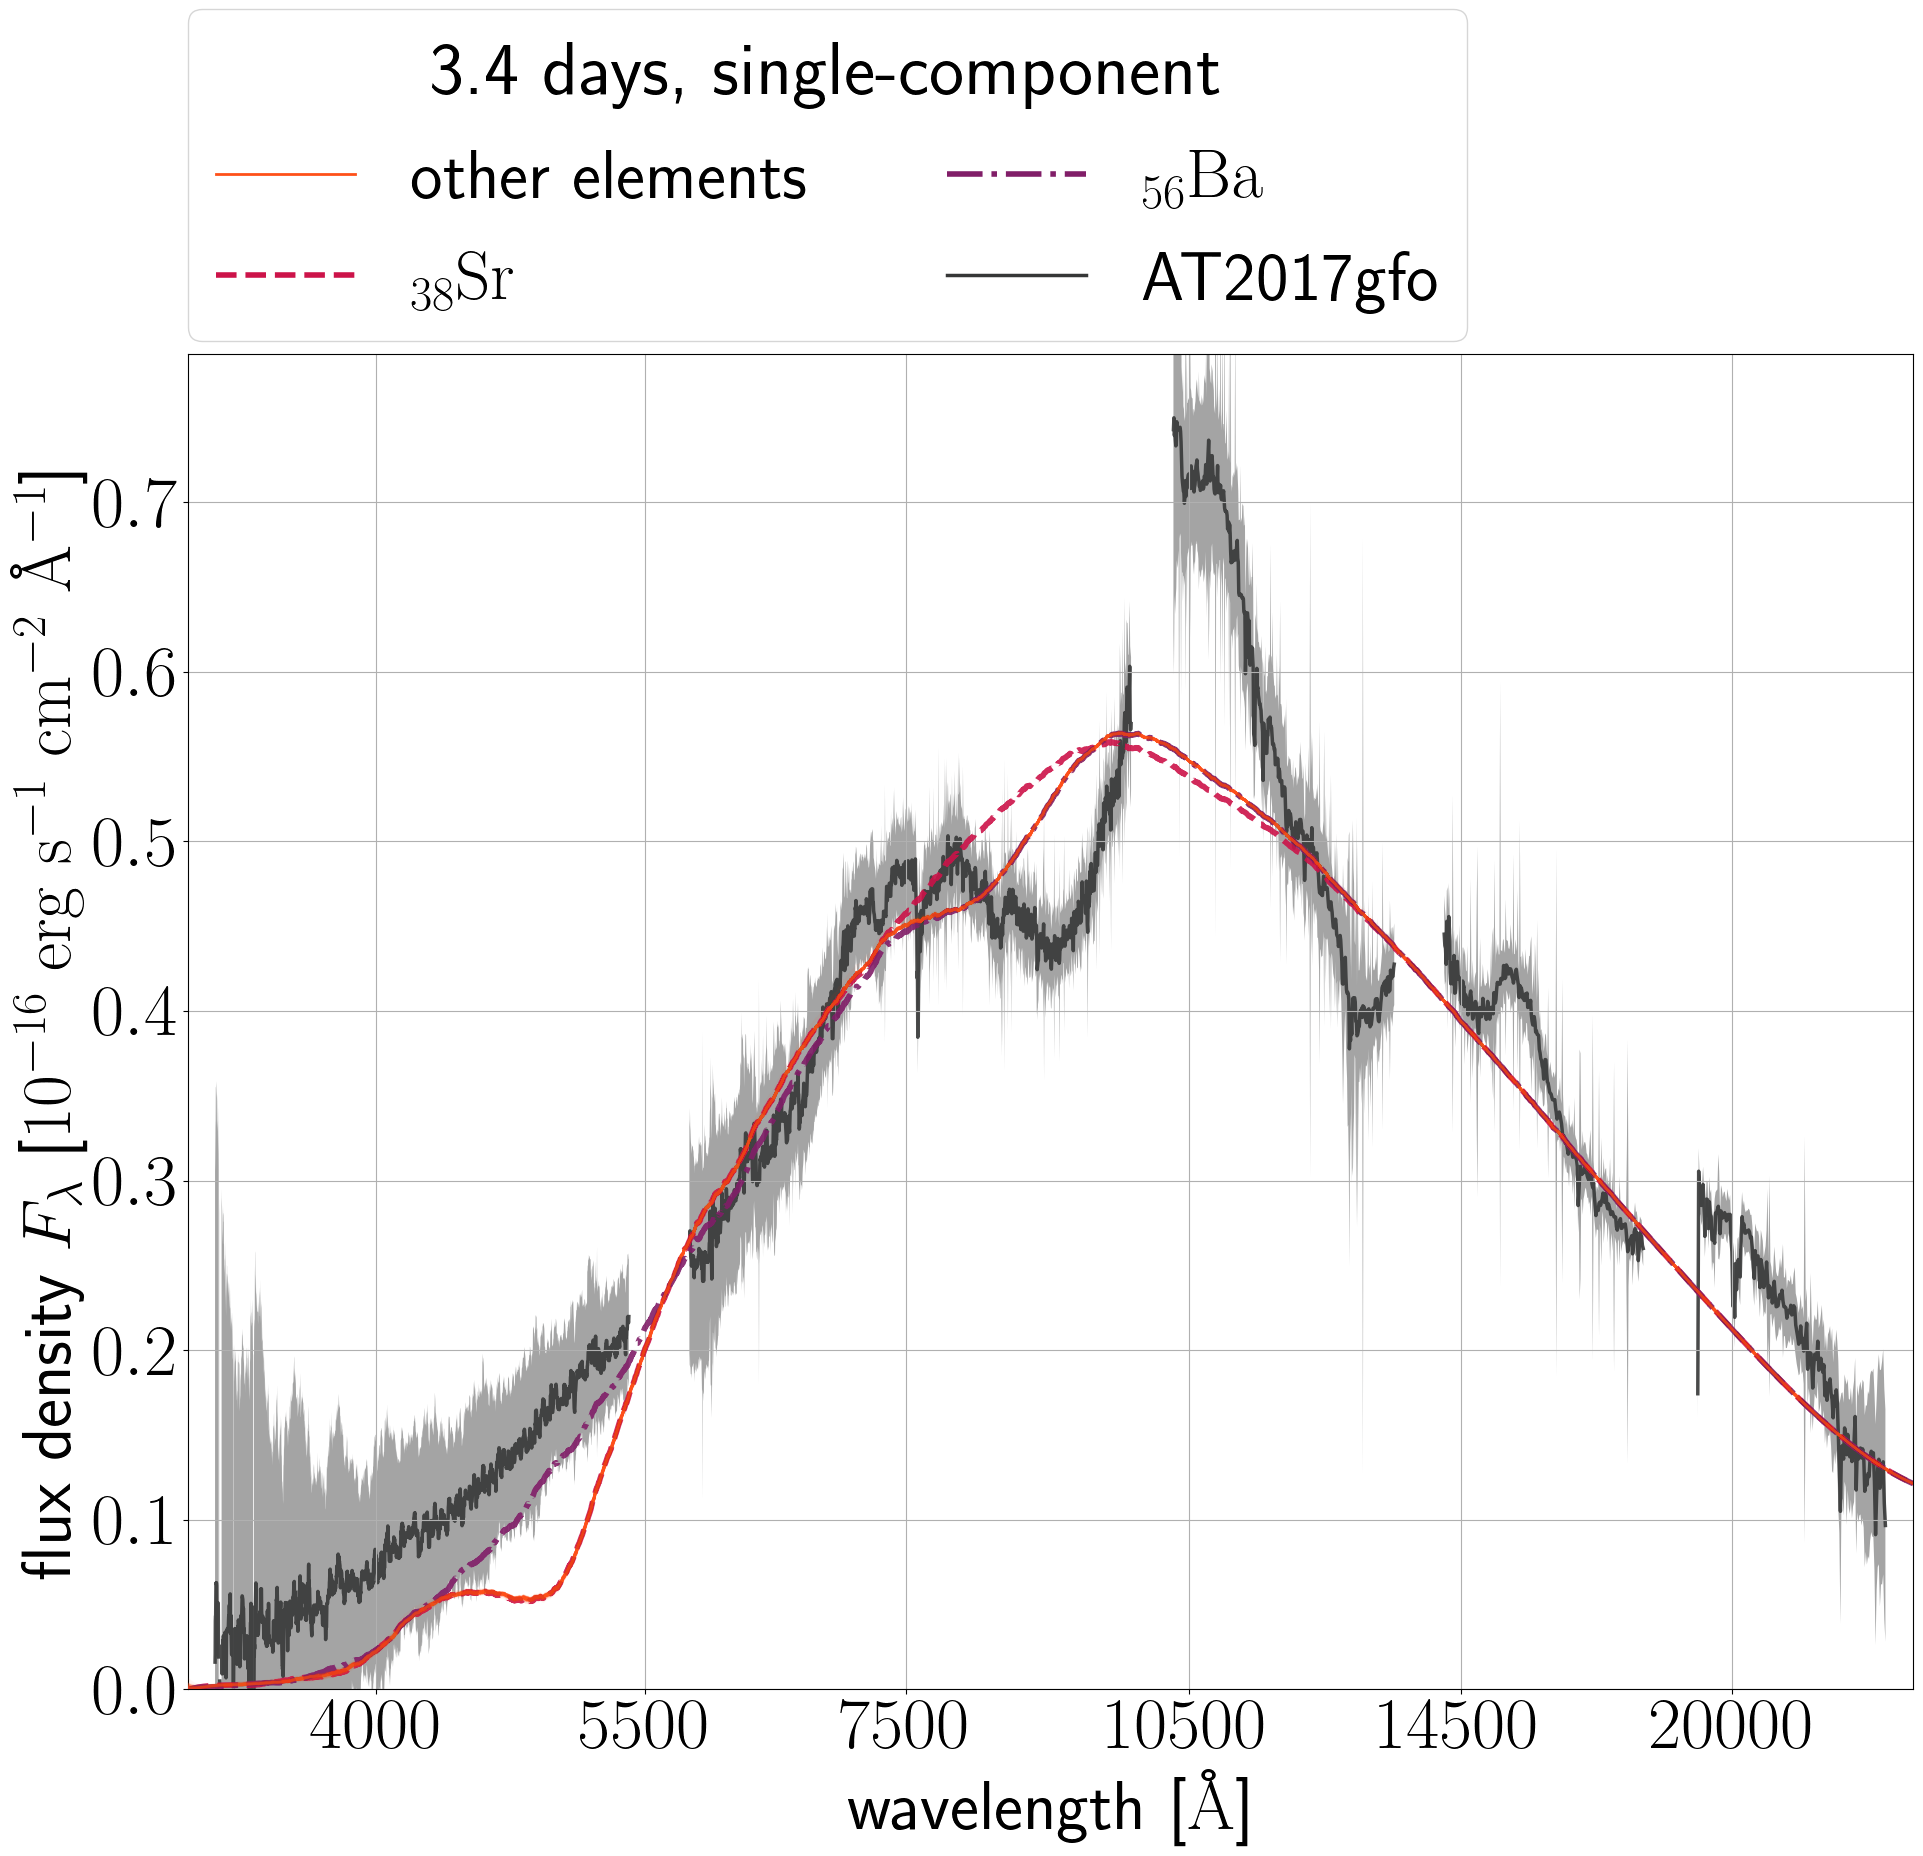
\includegraphics[width=0.47\textwidth]{figs/appendix/LoO/230628_205804_leaveoneout_all_TARDIS_evals_label-interest-38-56.png}
%     \figcaption{\textbf{Leave-one-out spectra for the disfavored models: multi-component for 1.4 and 2.4 days, and single-component for 3.4 days.} All models show clear absorption from strontium (${}_{38}$Sr) at $\sim8000$\AA. Both 1.4 and 2.4 day multi-component models also show absorption from yttrium (${}_{39}$Y). At (multi-component) 2.4 and (single-component) 3.4 days, absorption from barium (${}_{56}$Ba) is also present. Spectral DEComposition (SDEC) plots, included in Appendix~\ref{app:SDEC}, provide a complementary view of the dominant species to these leave-one-out plots.}\label{fig:leave_out_nonpref}
% \end{figure*}





%%% === APPENDIX C === %%%
%% SDEC %%
\section{Spectral DEComposition Plots}\label{app:SDEC}

Figure~\ref{fig:SDEC} shows the Spectral DEComposition (SDEC) plots for all 1.4, 2.4, and 3.4 day single- and multi-component fits. These SDEC plots show the species (elements or ions) which dominate the absorption (measured by absorbed luminosity) and emission (measured by emitted luminosity) in the spectrum. Above the $y = 0$ line, the height of the histogram indicates the total emitted luminosity in some wavelength bin, across different species. Below the $y = 0$ line, the depth of the histogram indicates the total absorbed luminosity. These plots also show how emission may be re-processed, \ie, absorbed in some wavelength range and reemmitted in another. These are complementary to the leave-one-out plots, which show which elements have the largest impact on the shape of the spectrum, in terms of either absorption or emission.

% \addstackgap SOLUTION INSPIRED BY [1]: https://tex.stackexchange.com/a/219766 
% \addstackgap SOLUTION INSPIRED BY [2]: https://tex.stackexchange.com/a/226335

\newlength{\SDECheight} % height of SDEC plots when printed out
\setlength{\SDECheight}{+5.6cm} % height of SDEC plots when printed out

\begin{figure*}[!ht]
    \centering
    \begin{tabular}{ccc}
    single-component & multi-component & \\
    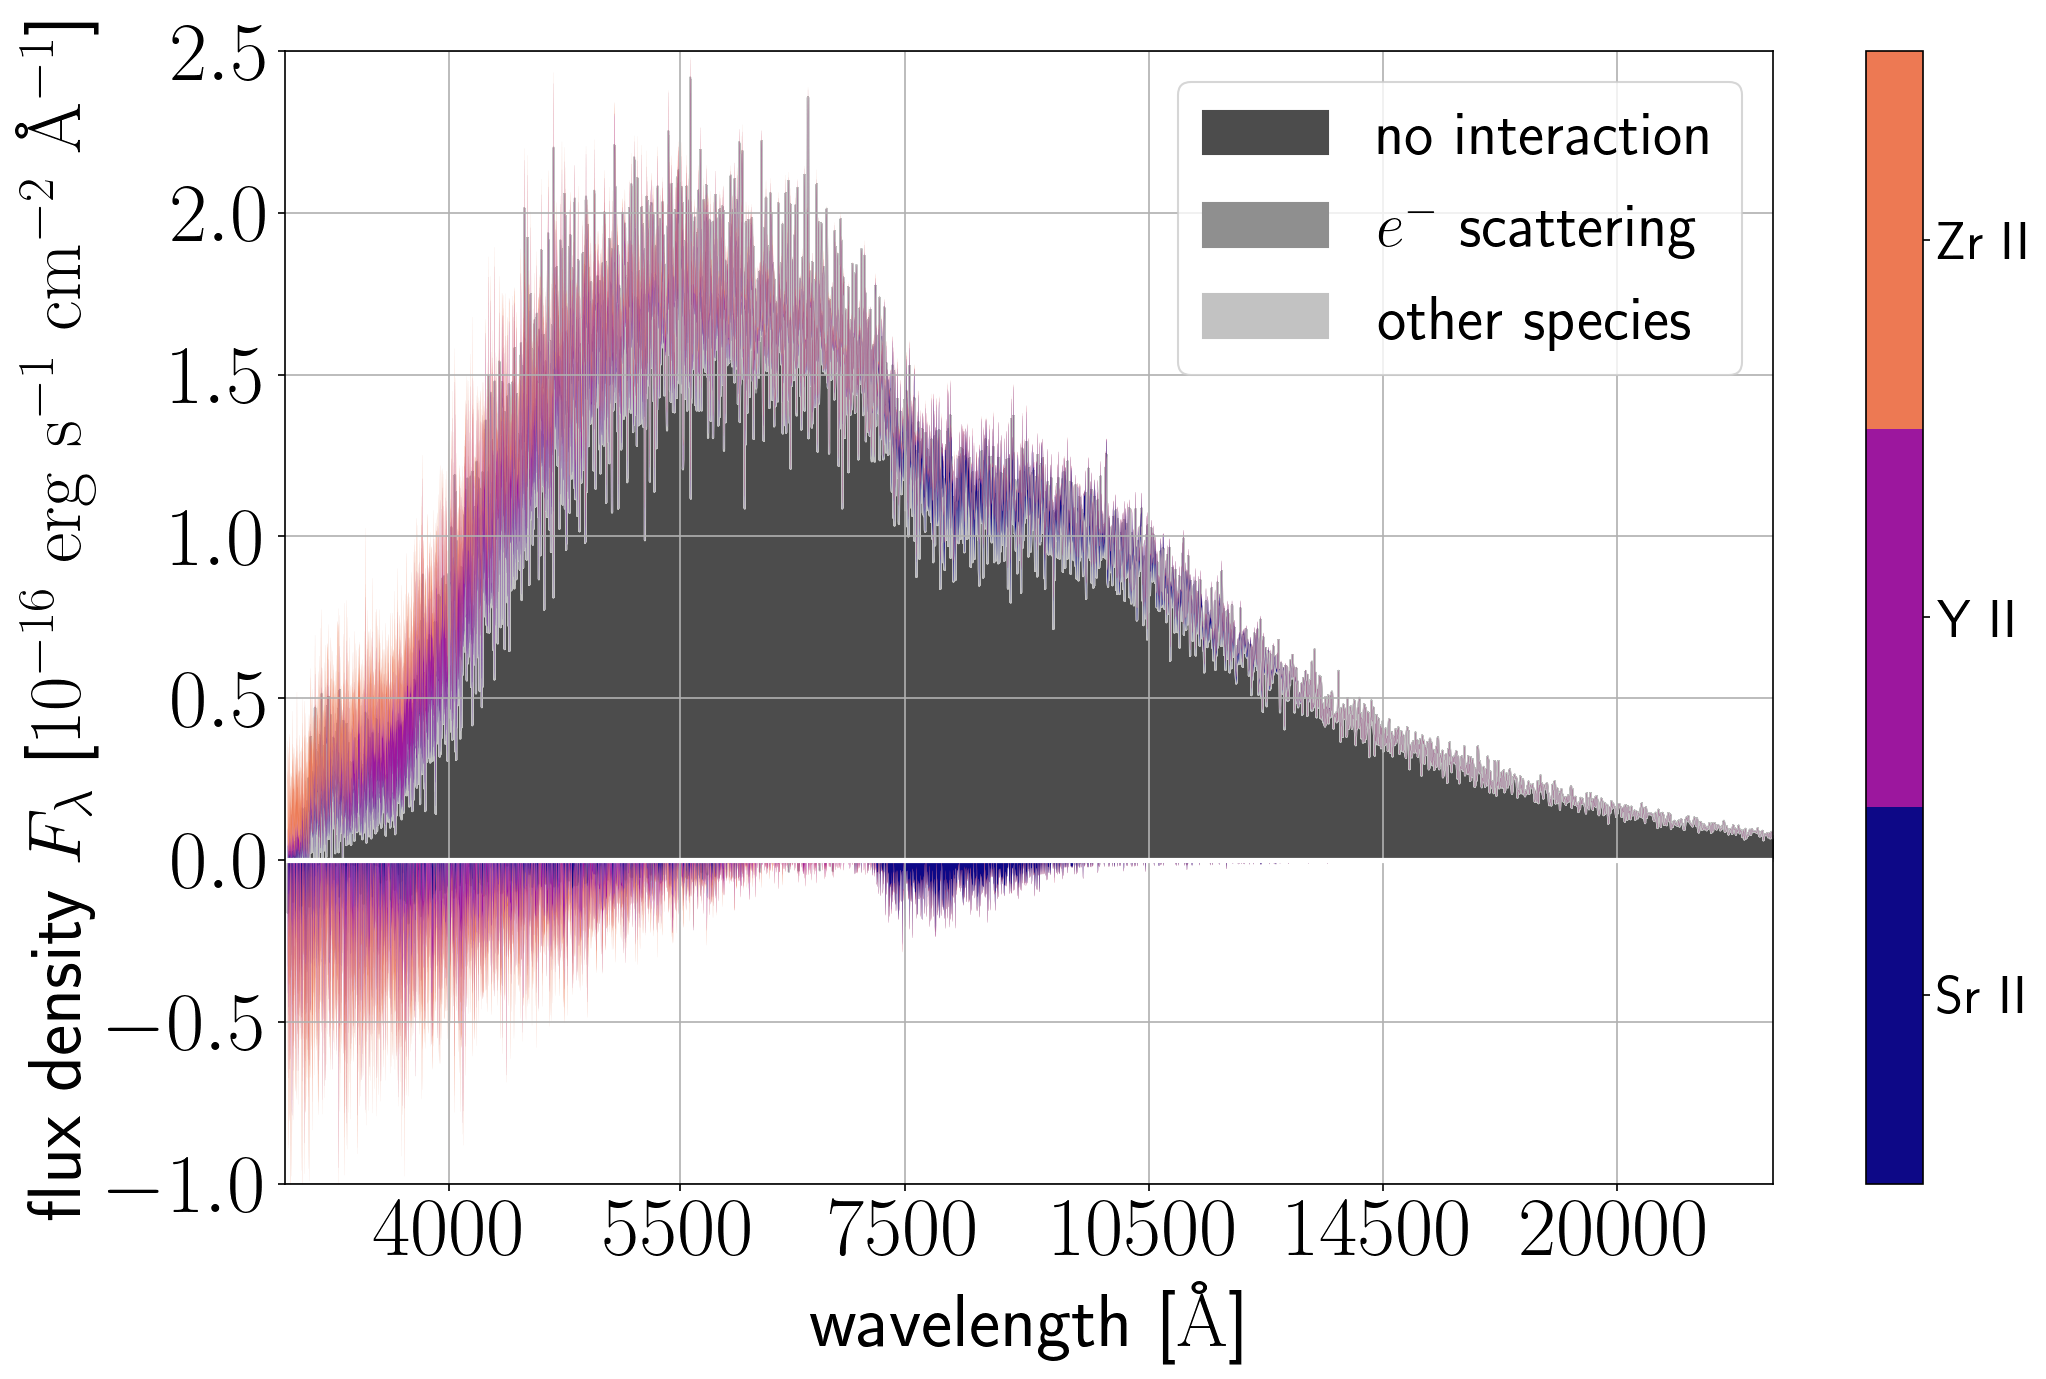
\includegraphics[width=0.47\textwidth]{figs/appendix/SDEC/230704_165812_single_TARDIS_eval_SDEC.png} & 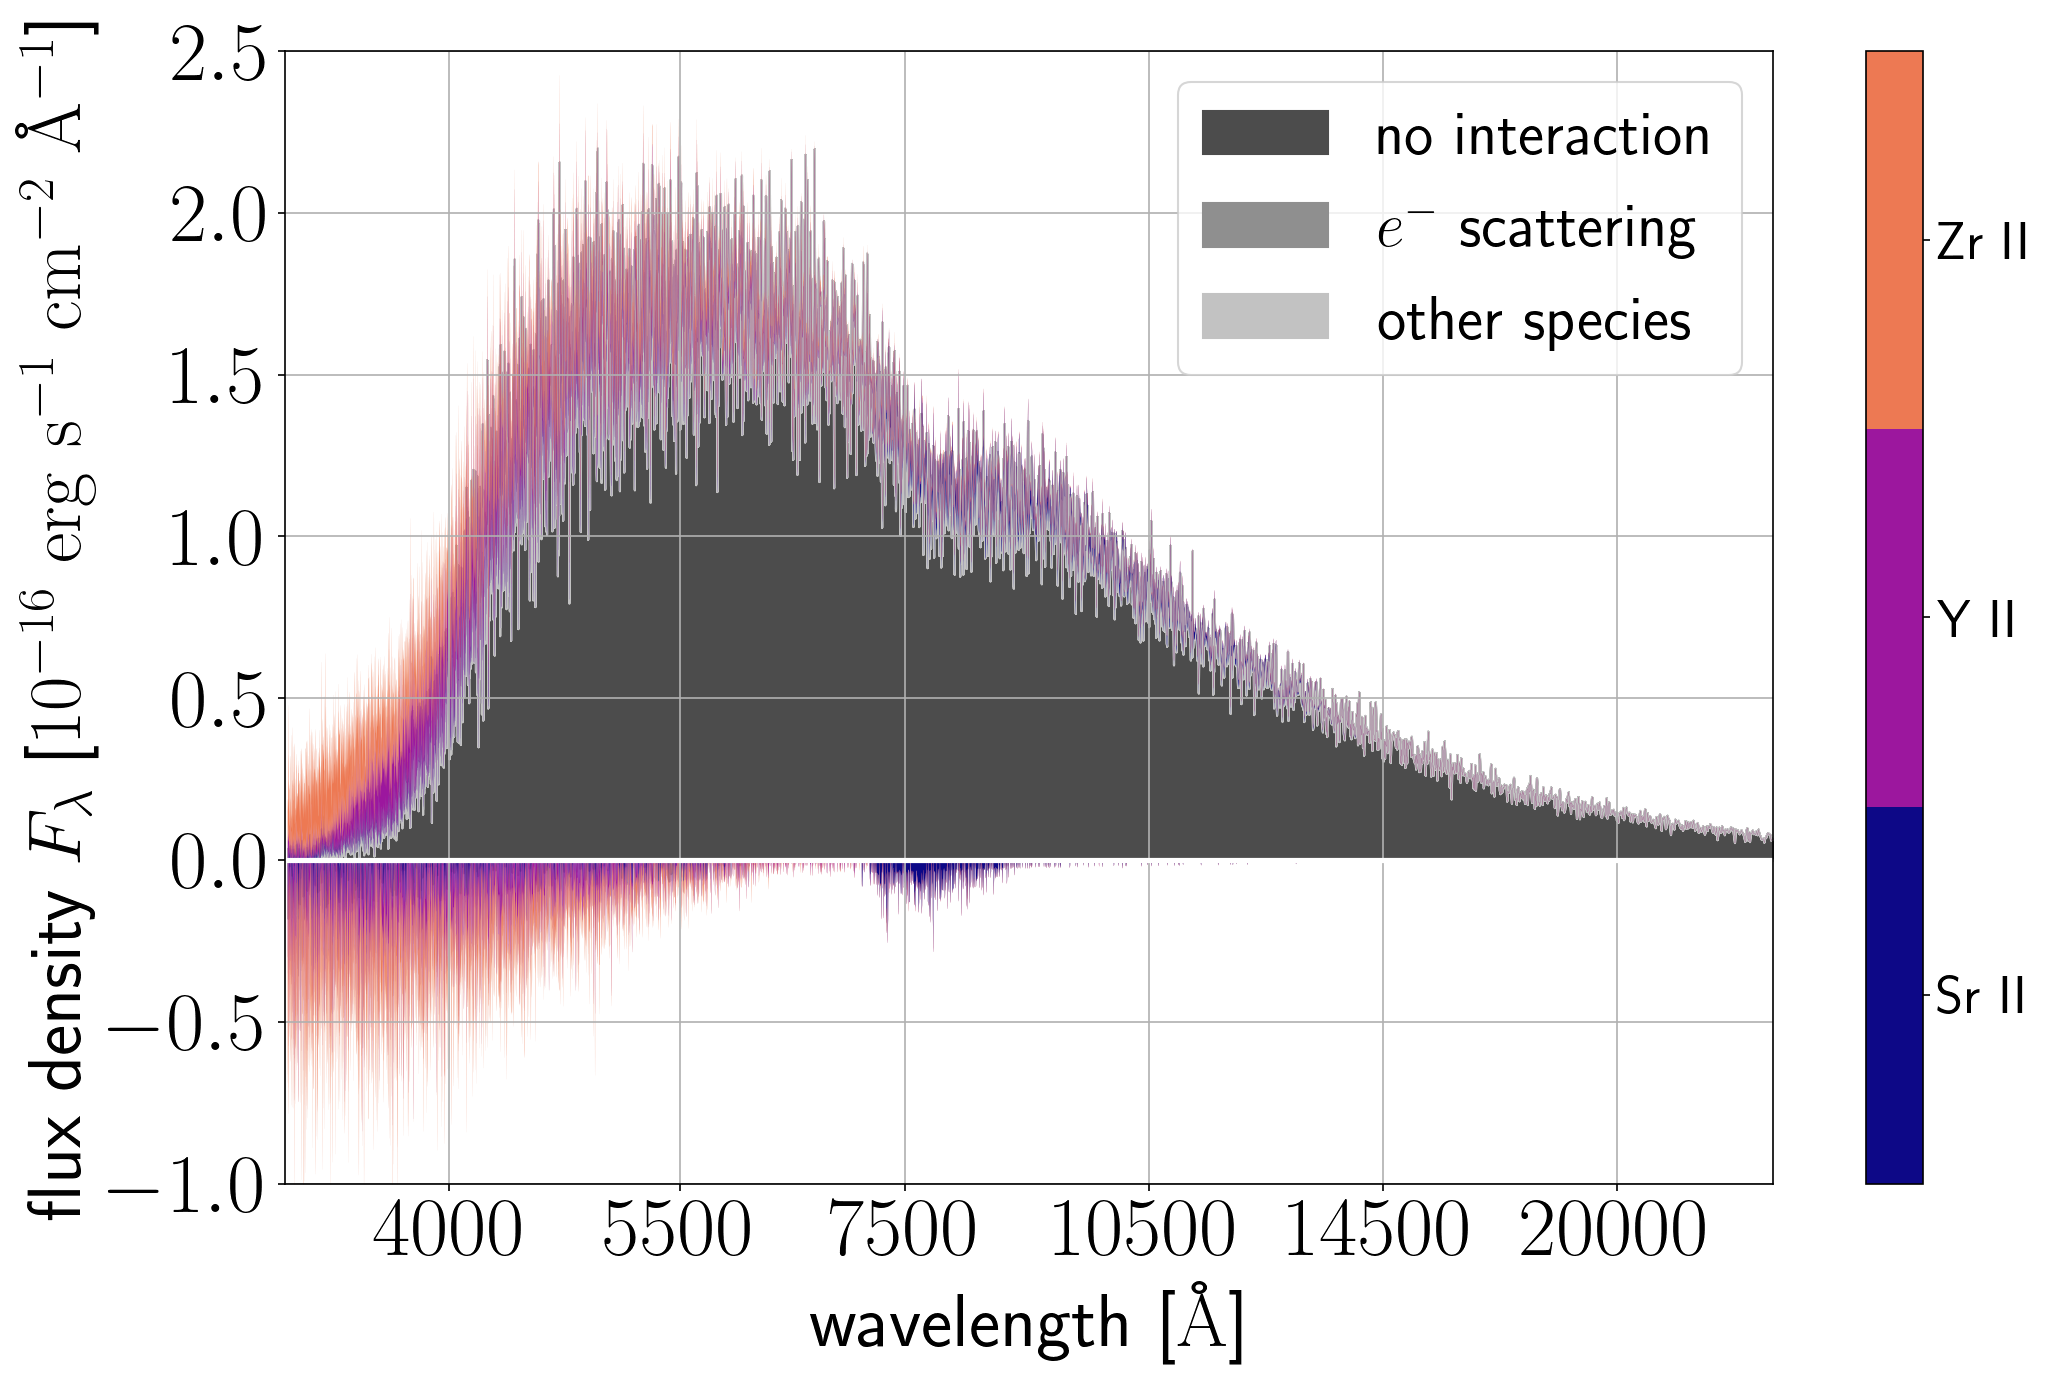
\includegraphics[width=0.47\textwidth] {figs/appendix/SDEC/230726_113032_single_TARDIS_eval_SDEC.png} & \addstackgap{\raisebox{0.5\SDECheight}{1.4 days}} \\
    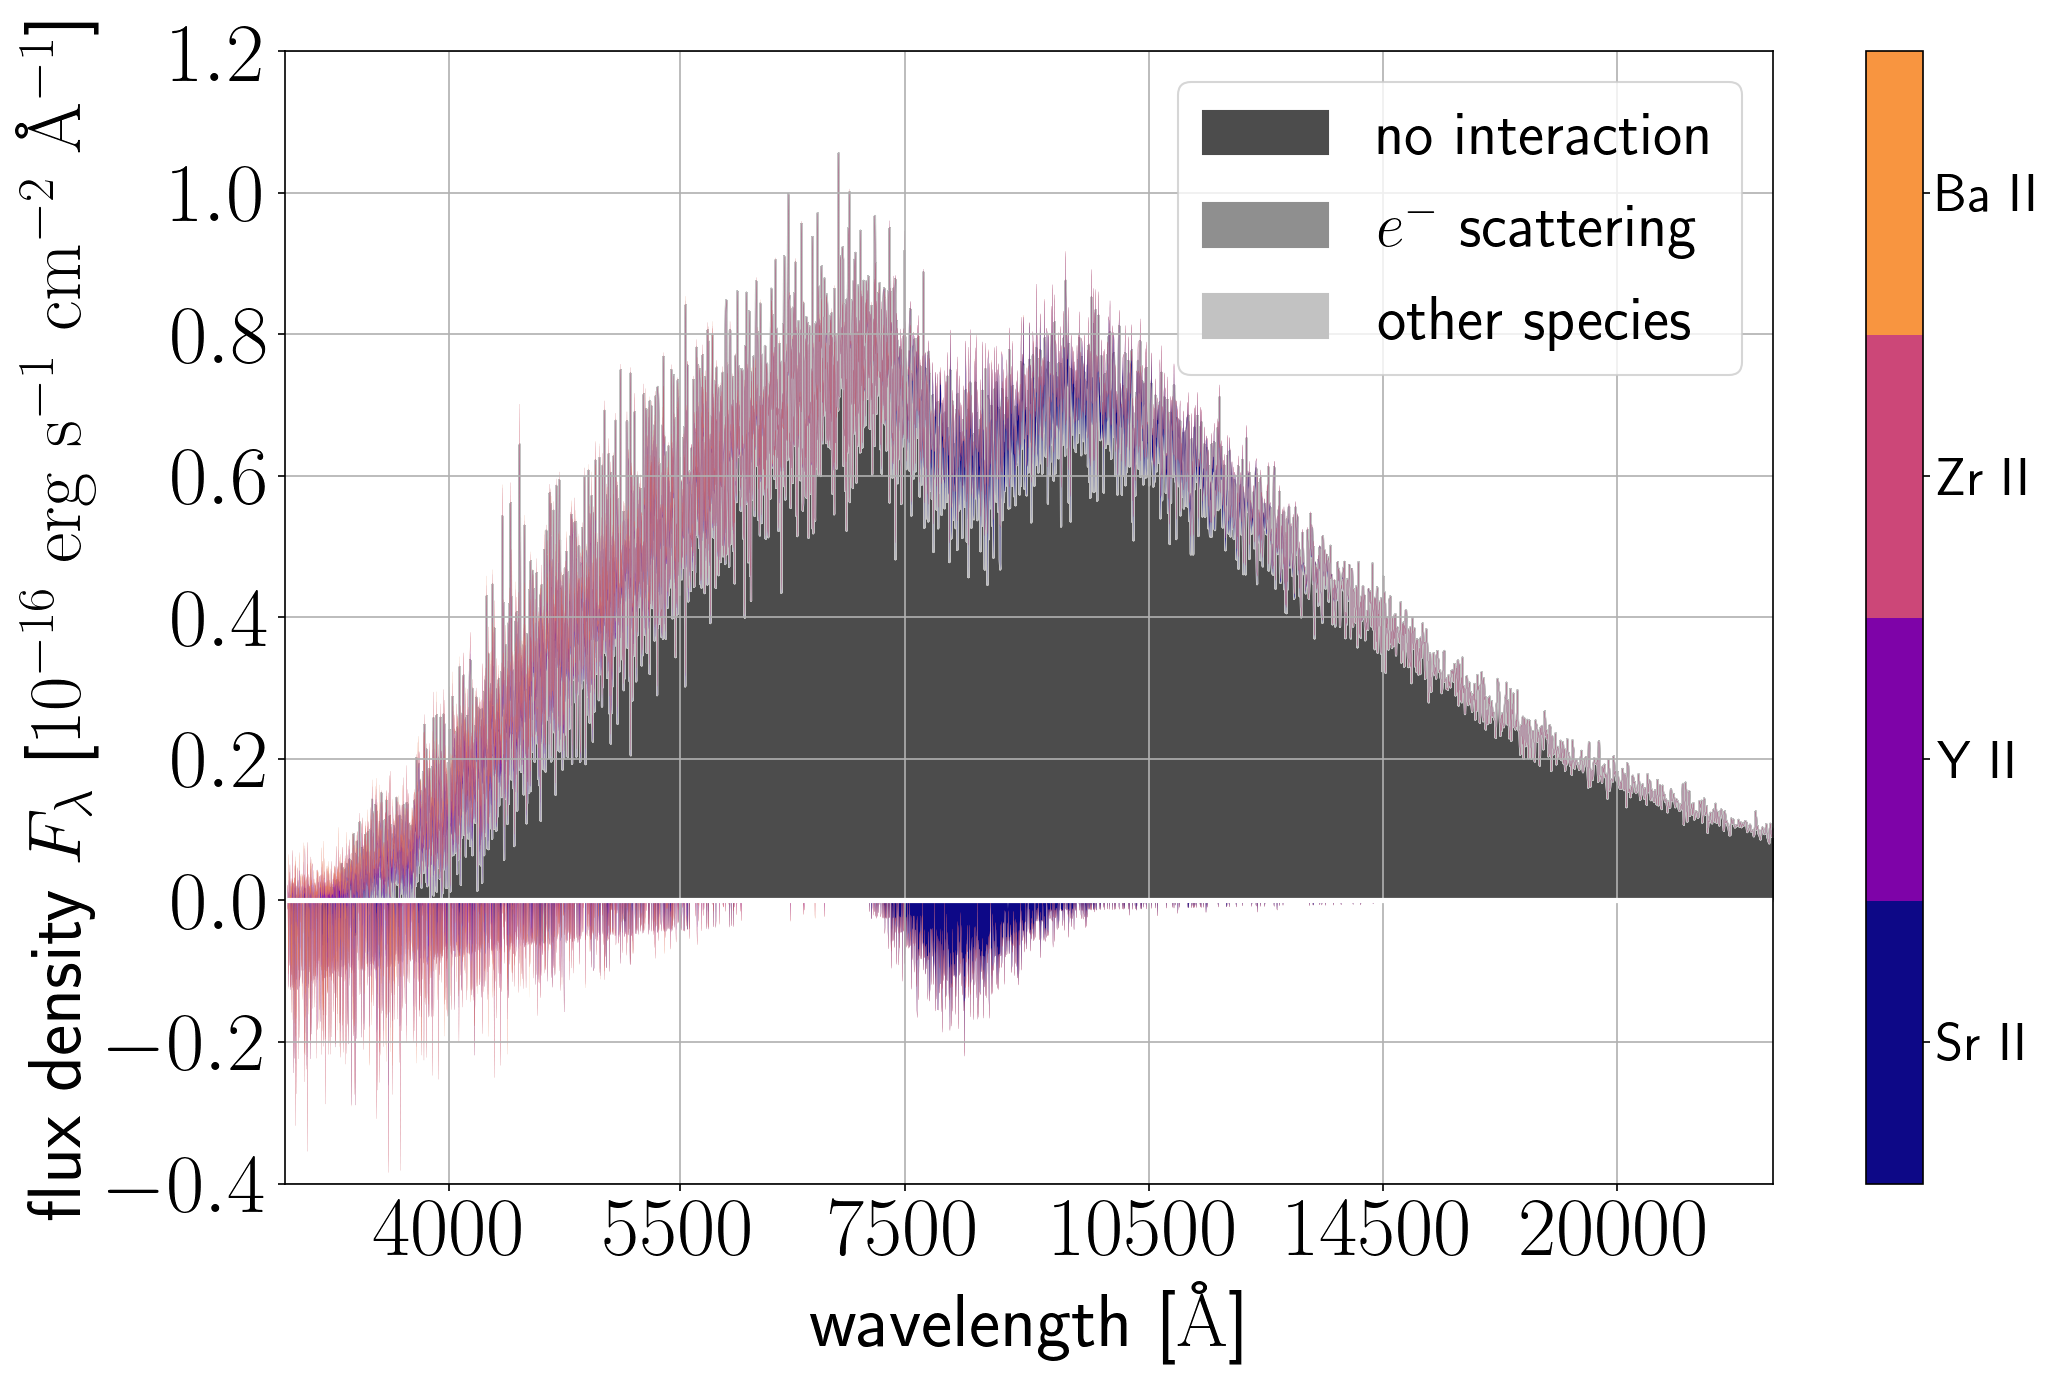
\includegraphics[width=0.47\textwidth]{figs/appendix/SDEC/221024_080947_single_TARDIS_eval_SDEC.png} & 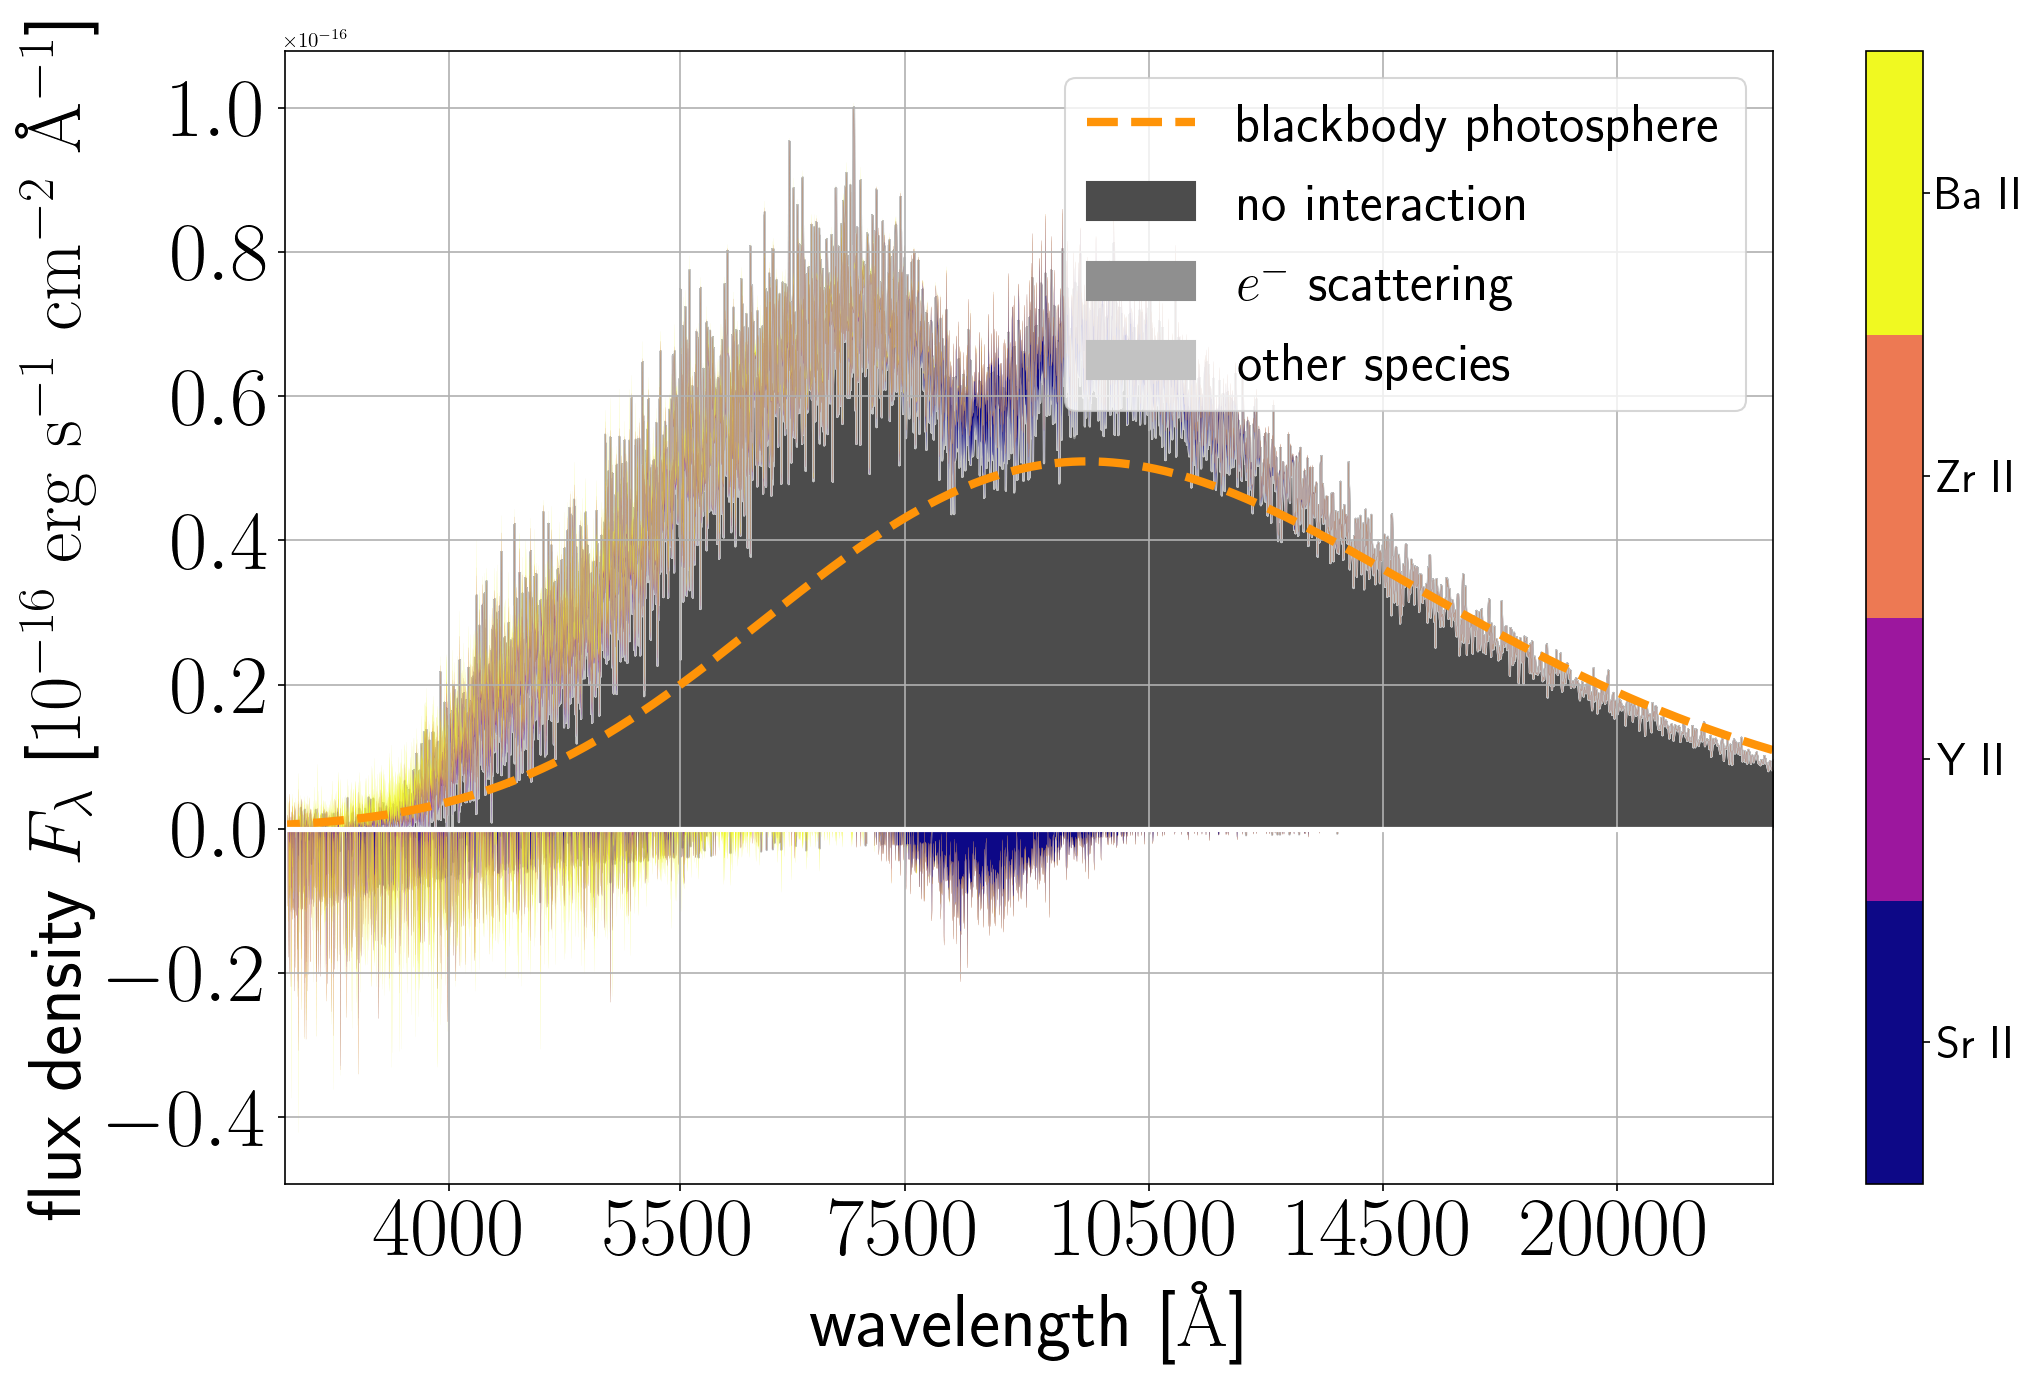
\includegraphics[width=0.47\textwidth] {figs/appendix/SDEC/230412_035244_single_TARDIS_eval_SDEC.png} & \addstackgap{\raisebox{0.5\SDECheight}{2.4 days}} \\ 
    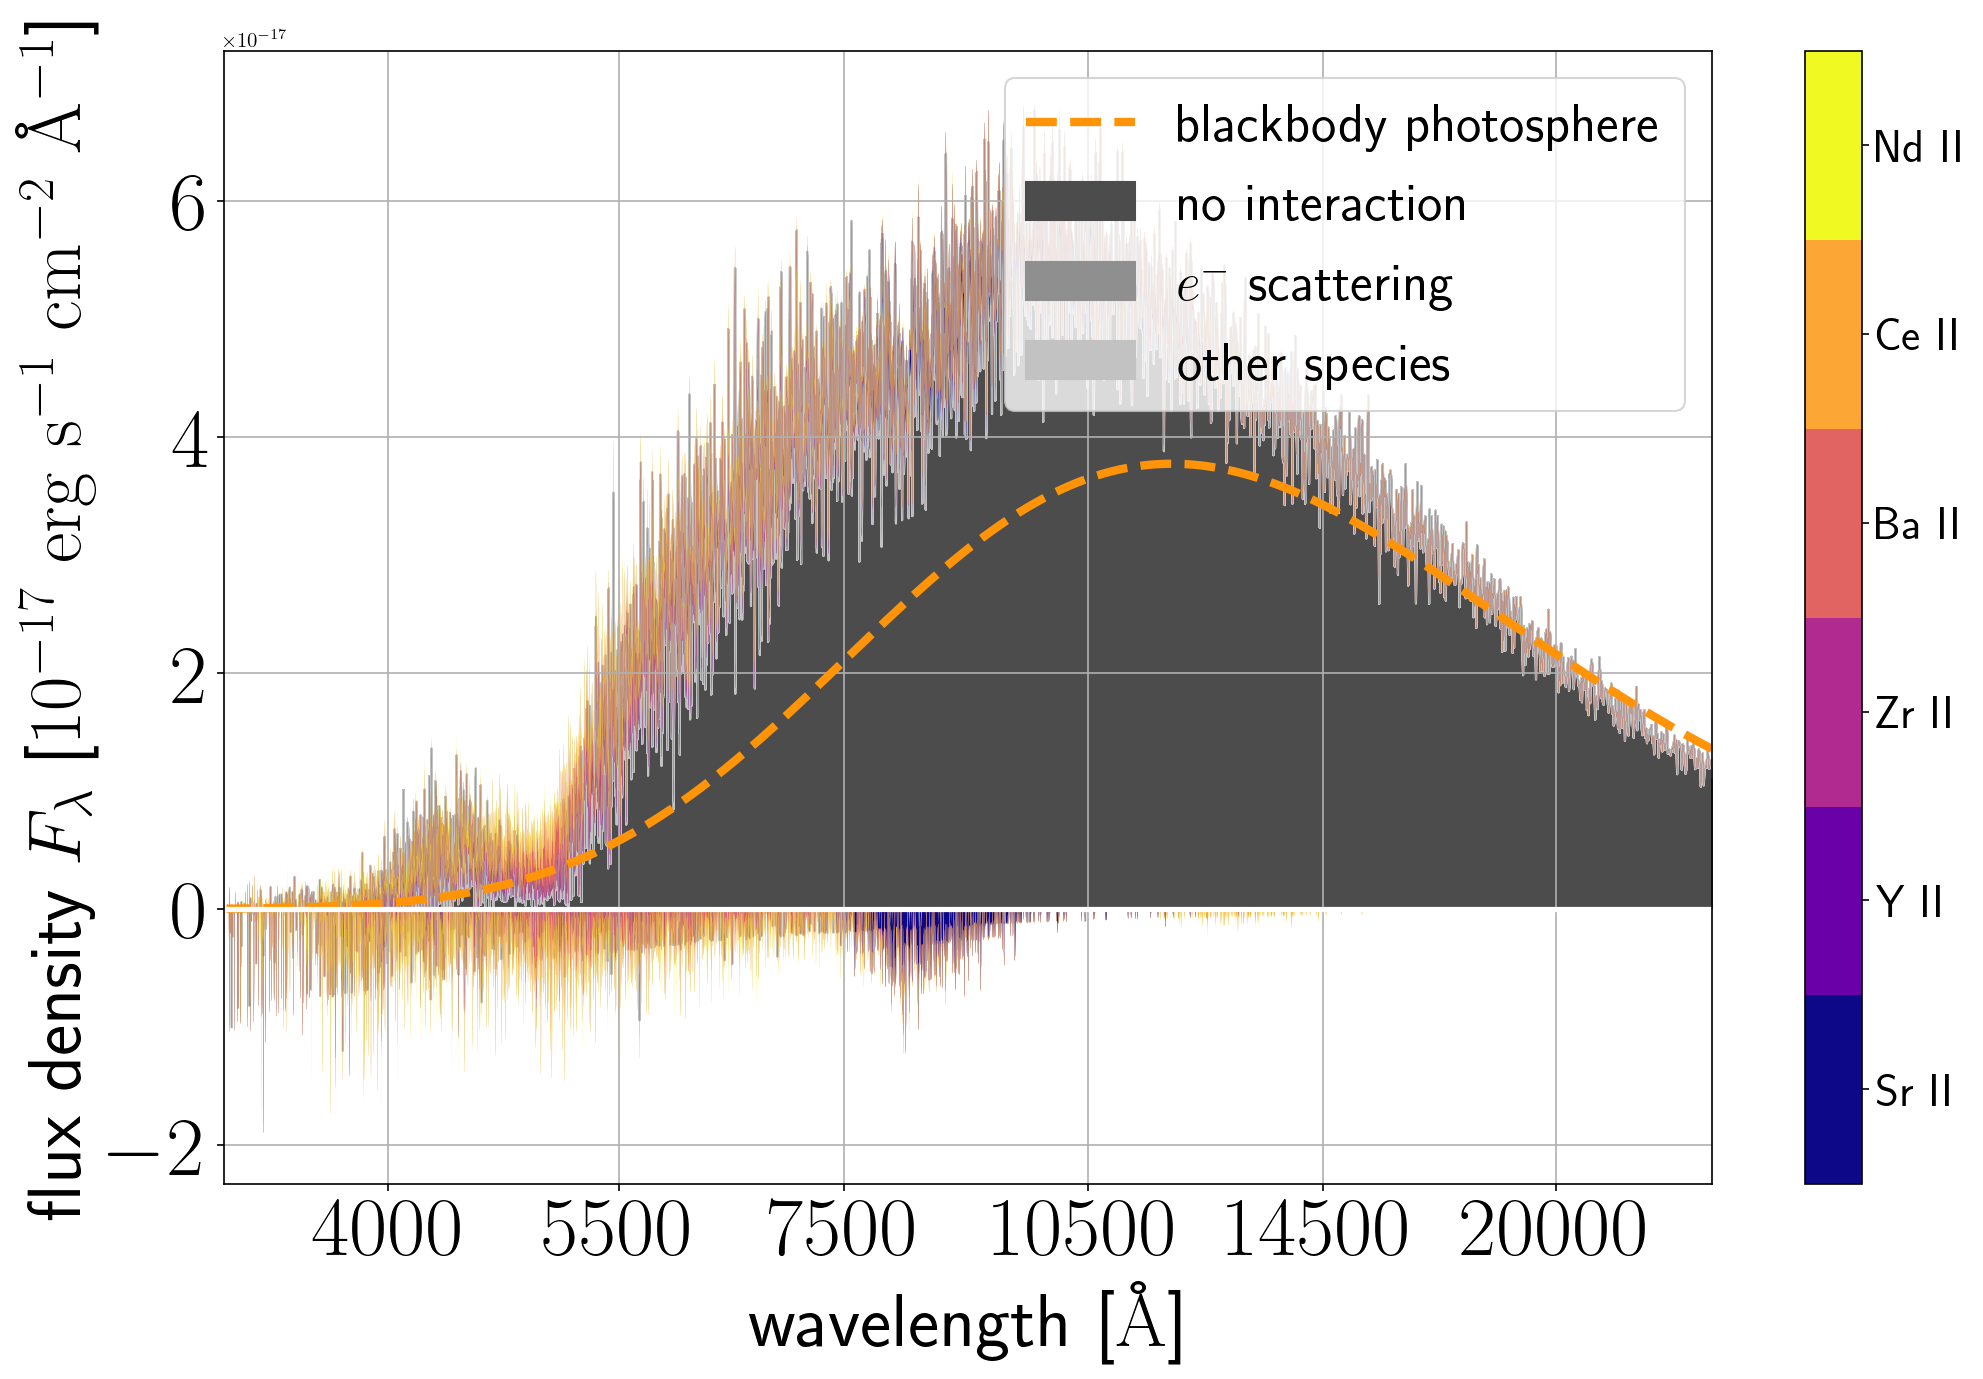
\includegraphics[width=0.47\textwidth]{figs/appendix/SDEC/230621_082134_single_TARDIS_eval_SDEC.png} & 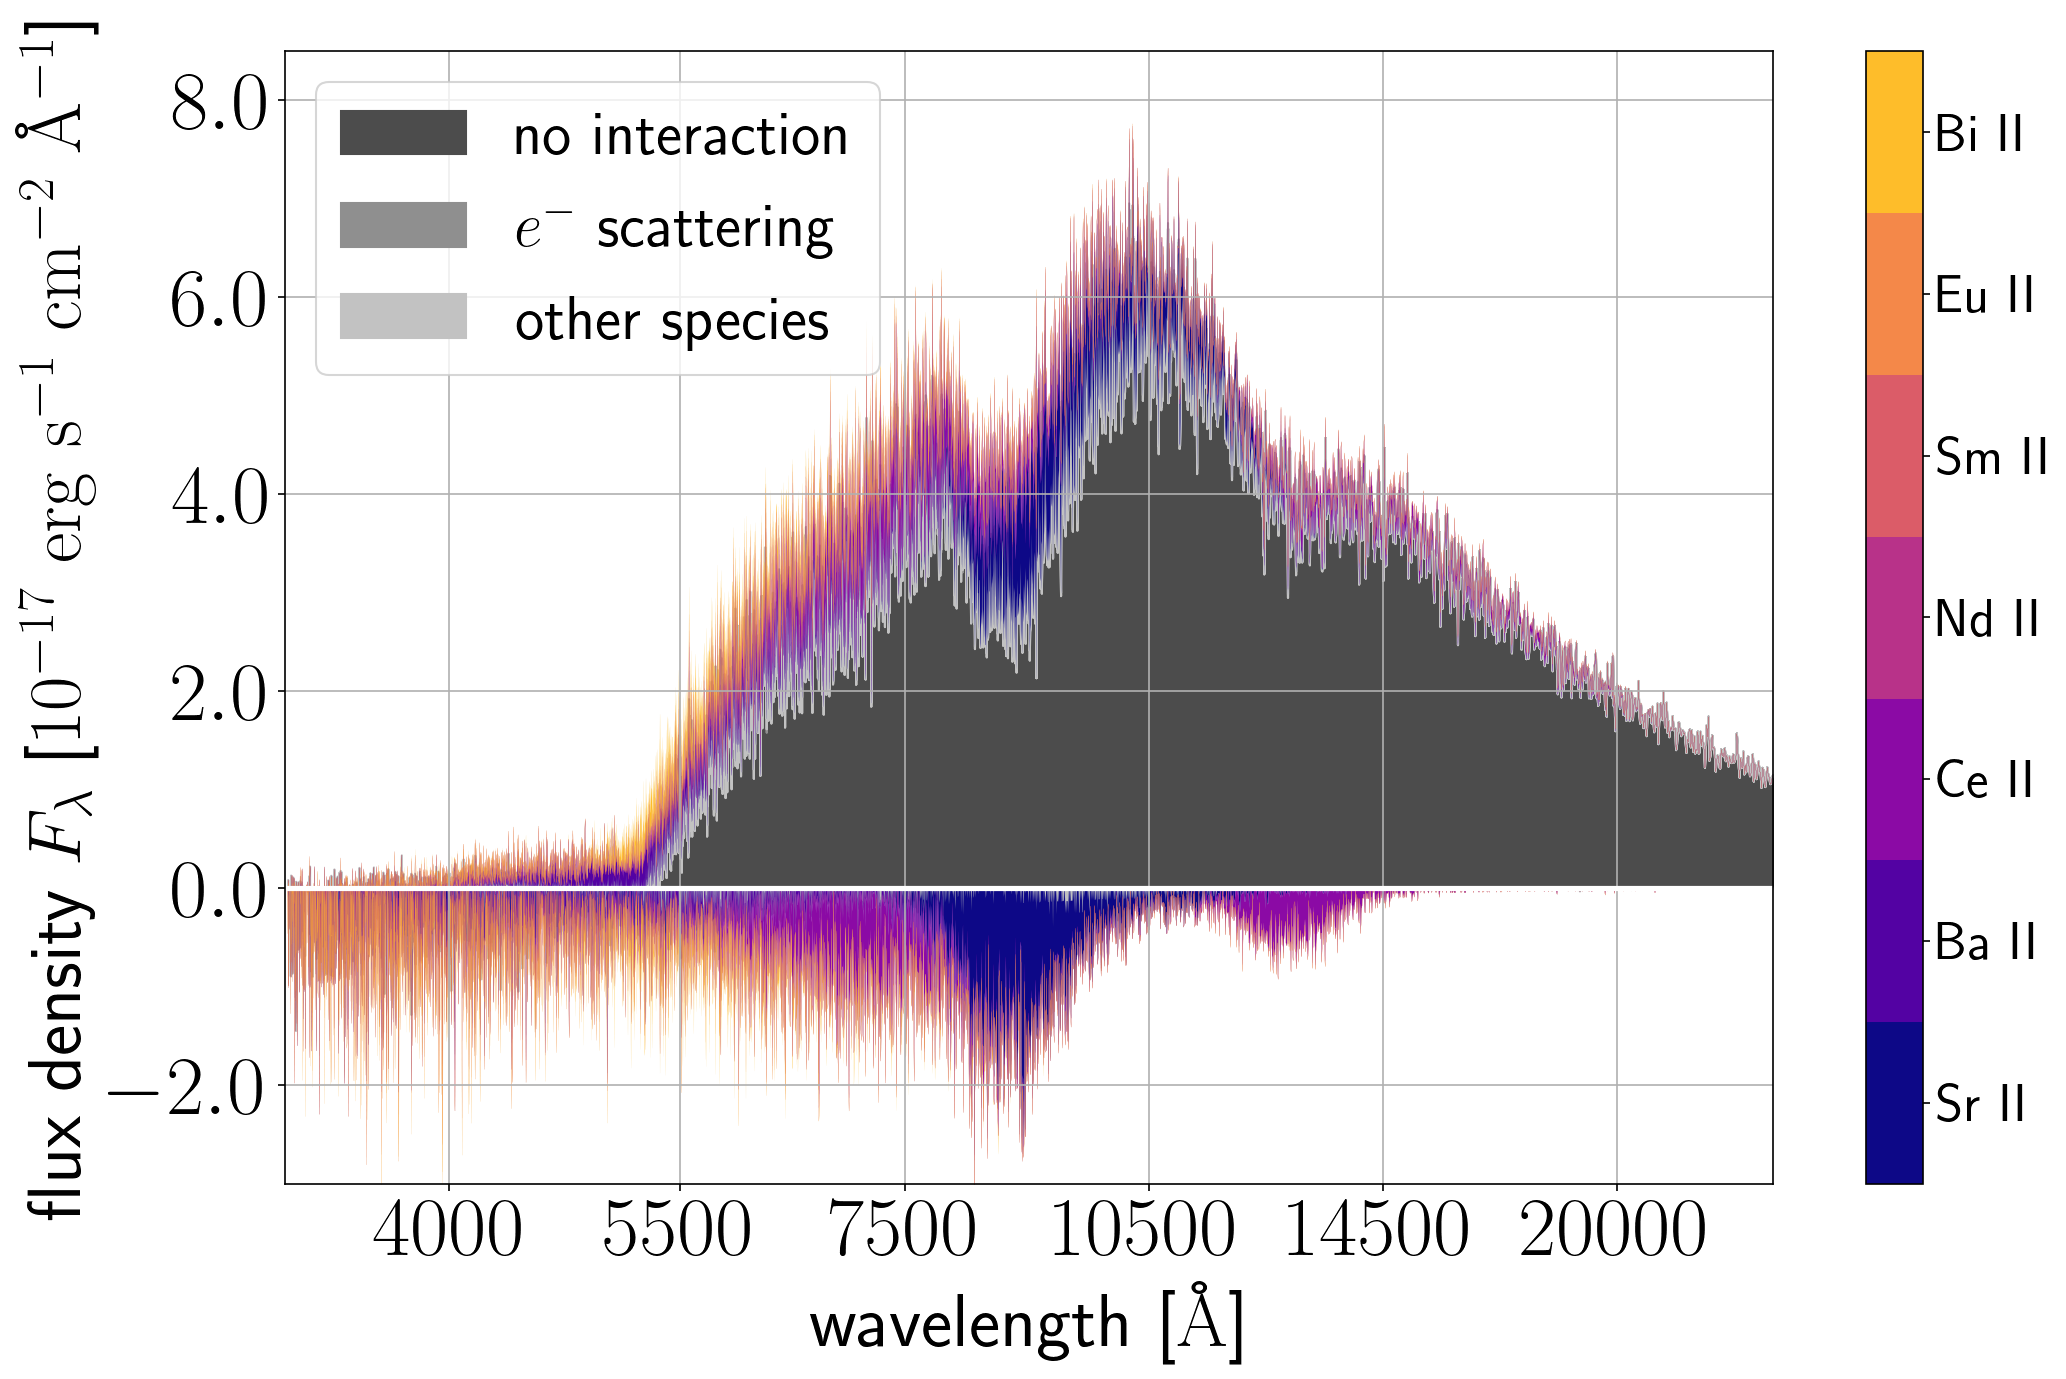
\includegraphics[width=0.47\textwidth] {figs/appendix/SDEC/230626_073230_single_TARDIS_eval_SDEC.png} & \addstackgap{\raisebox{0.5\SDECheight}{3.4 days}} \\
    \end{tabular}
    \figcaption{\textbf{Spectral DEComposition (SDEC) plots for all best fits, at 1.4, 2.4, and 3.4 days, for single- and multi-component models}. The left column contains single-component models for 1.4, 2.4, and 3.4 days; the right contains multi-component equivalents. The ions \ion{Sr}{2}, \ion{Y}{2}, and \ion{Zr}{2} produce significant absorption in all 1.4 day and 2.4 day models. The 2.4 day models also show absorption from \ion{Ba}{2}. The 3.4 day single-component model (which is a poor fit to the observed spectrum, but nonetheless the best fit possible with a single component) exhibits absorption from all four of these ions, except \ion{Zr}{1} in the place of \ion{Zr}{2}, due to the cooler ejecta. The spectrum also shows moderate absorption from ions of three lanthanides: \ion{La}{2}, \ion{Ce}{2}, and \ion{Nd}{2}. The 3.4 multi-component model, which is favored over the single-component, shows absorption from two open $s$-shell elements in the same periodic table group (\ion{Sr}{2} and \ion{Ba}{2}), four lanthanide ions (\ion{Ce}{2}, \ion{Nd}{2}, \ion{Sm}{2}, and \ion{Eu}{2}), and one ion of an especially heavy element, \ion{Bi}{2}. Furthermore, unlike at earlier epochs, ions of Y and Zr do not dominate absorption in the 3.4 day multi-component model.}\label{fig:SDEC}
\end{figure*}





%%% === APPENDIX D === %%%
%% CONVERGENCE OF FITS %%
\section{Convergence of fits}\label{app:convergence}

We assess the convergence of each fit using the \approxposterior~$z$ convergence diagnostic:

\begin{equation}
    z_{t,j} = \frac{\mu_{t,j} - \mu_{t-1,j}}{\sigma_{t-1,j}},
\end{equation}\label{eqn:convergence_z}

\noindent where $\mu_{t,j}$ and $\sigma_{t,j}$ are the mean and standard deviation of the posterior for model parameter $\theta_j$ at the $t$'th instance of nested sampling. This diagnostic thus assesses the stability of the posterior as more active learning samples are added to the training set of the GP. Figure~\ref{fig:convergence_single} shows these convergence plots for single-component runs at 1.4, 2.4, and 3.4 days; Figure~\ref{fig:convergence_multi} shows the multi-component equivalents. We define convergence as $z_{t,j} \leqslant 0.5$ for all $j$ for sufficient consecutive iterations. In all cases, convergence is obtained, and the final posterior is stable as more active learning samples are added to the training set.


\begin{figure*}[!ht]
    \centering
    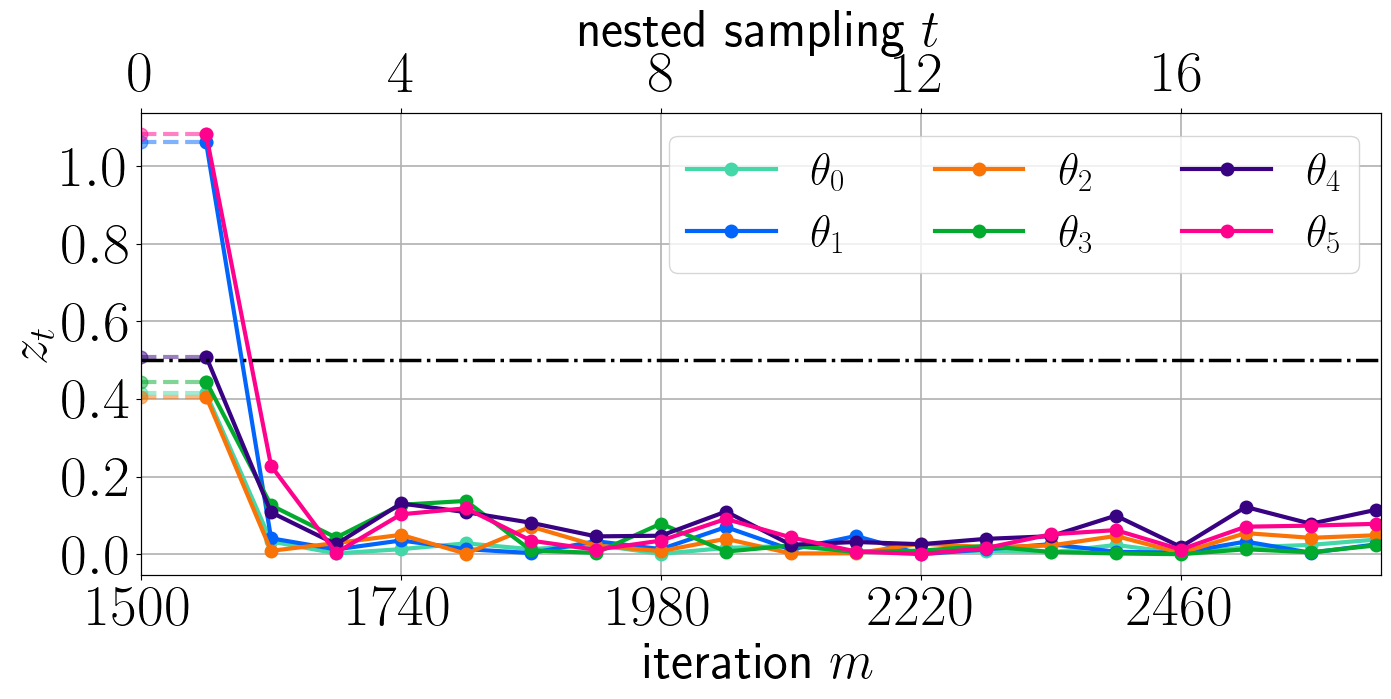
\includegraphics[width=0.8\textwidth]{figs/appendix/convergence/220808_014638_dynesty-sampling_convergence_z_eps0.5.png}
    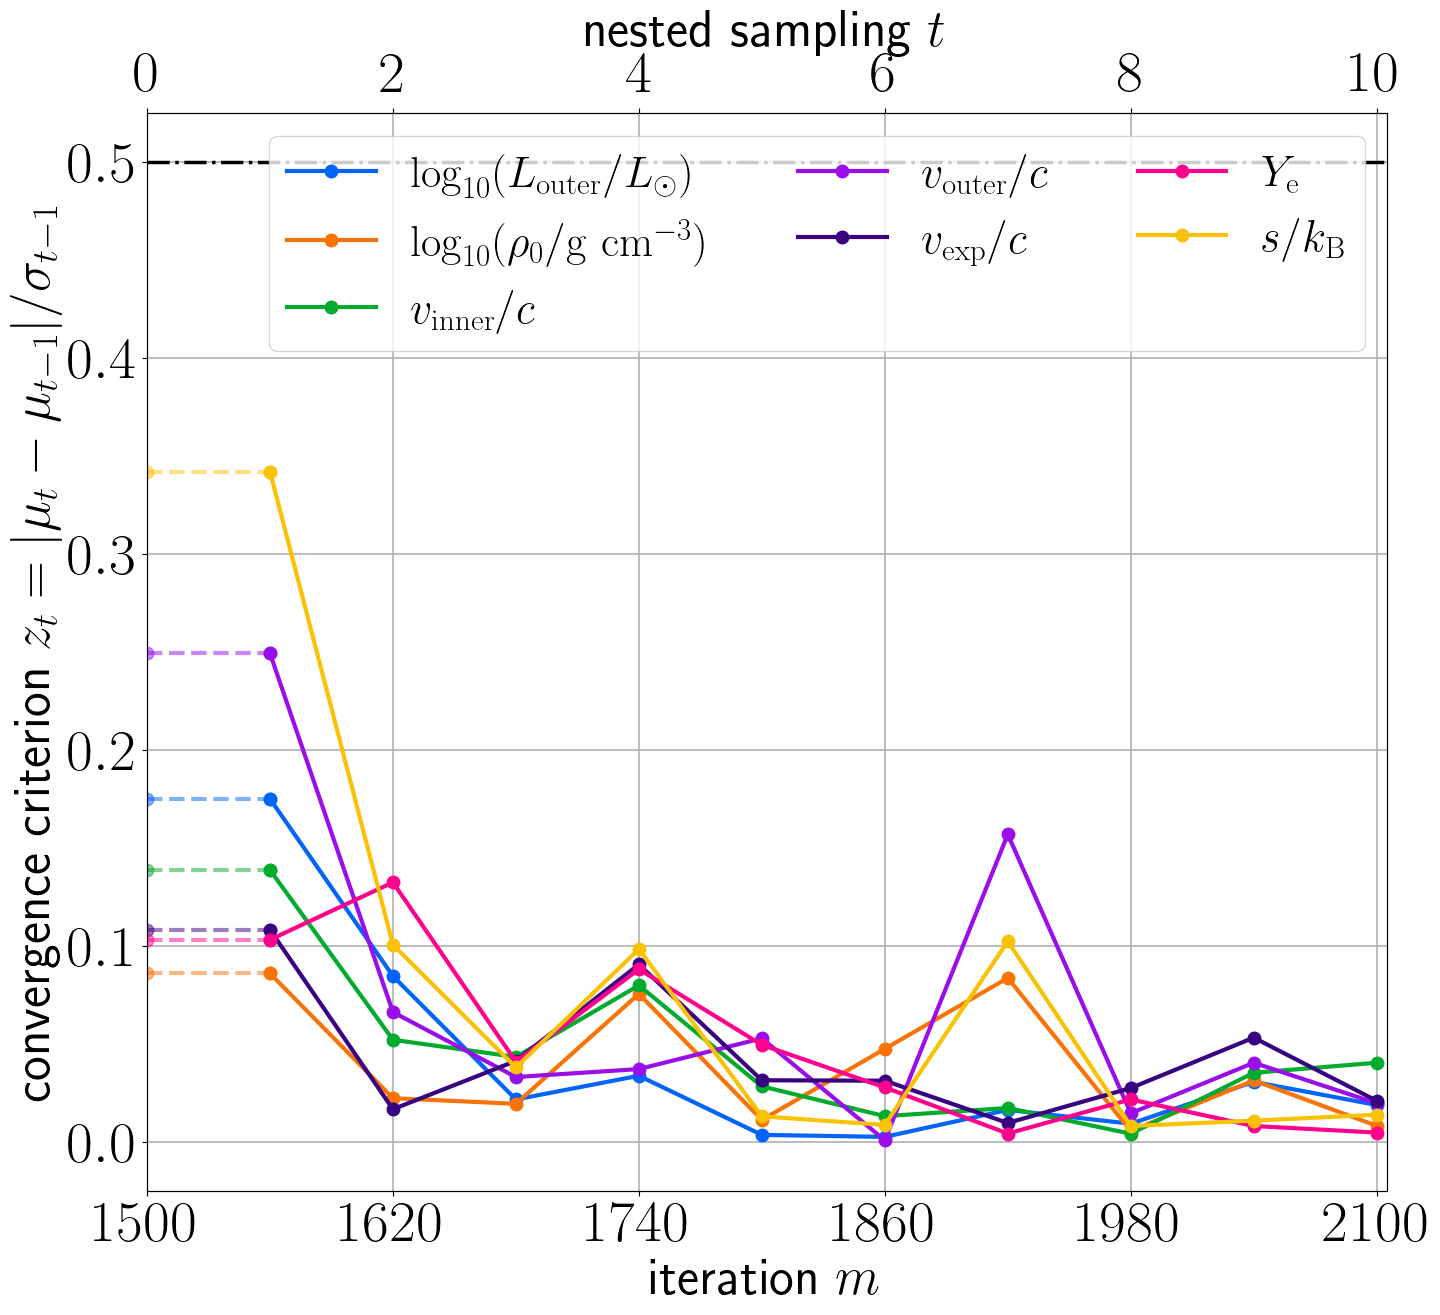
\includegraphics[width=0.8\textwidth]{figs/appendix/convergence/221022_084052_dynesty-sampling_convergence_z_eps0.5.png}
    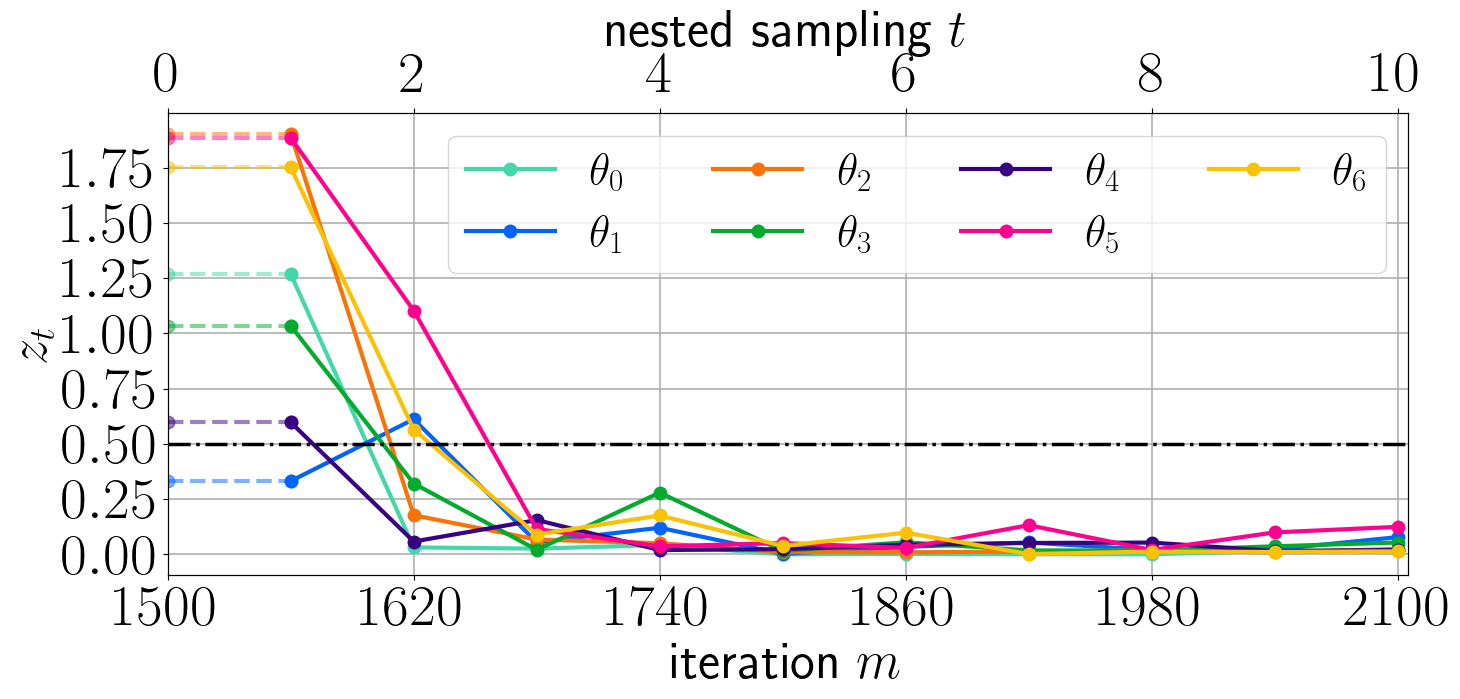
\includegraphics[width=0.8\textwidth]{figs/appendix/convergence/230618_143307_dynesty-sampling_convergence_z_eps0.5.png}
    \figcaption{\textbf{Convergence of the GP, measured according to the $z$ \approxposterior~convergence diagnostic, for the single-component runs at 1.4, 2.4, and 3.4 days.} We define convergence as $z_{t,j} \leqslant 0.5$ for all $j$ for sufficient consecutive iterations (see Equation~\ref{eqn:convergence_z}). In all cases, convergence is obtained.}\label{fig:convergence_single}
\end{figure*}

\begin{figure*}[!ht]
    \centering
    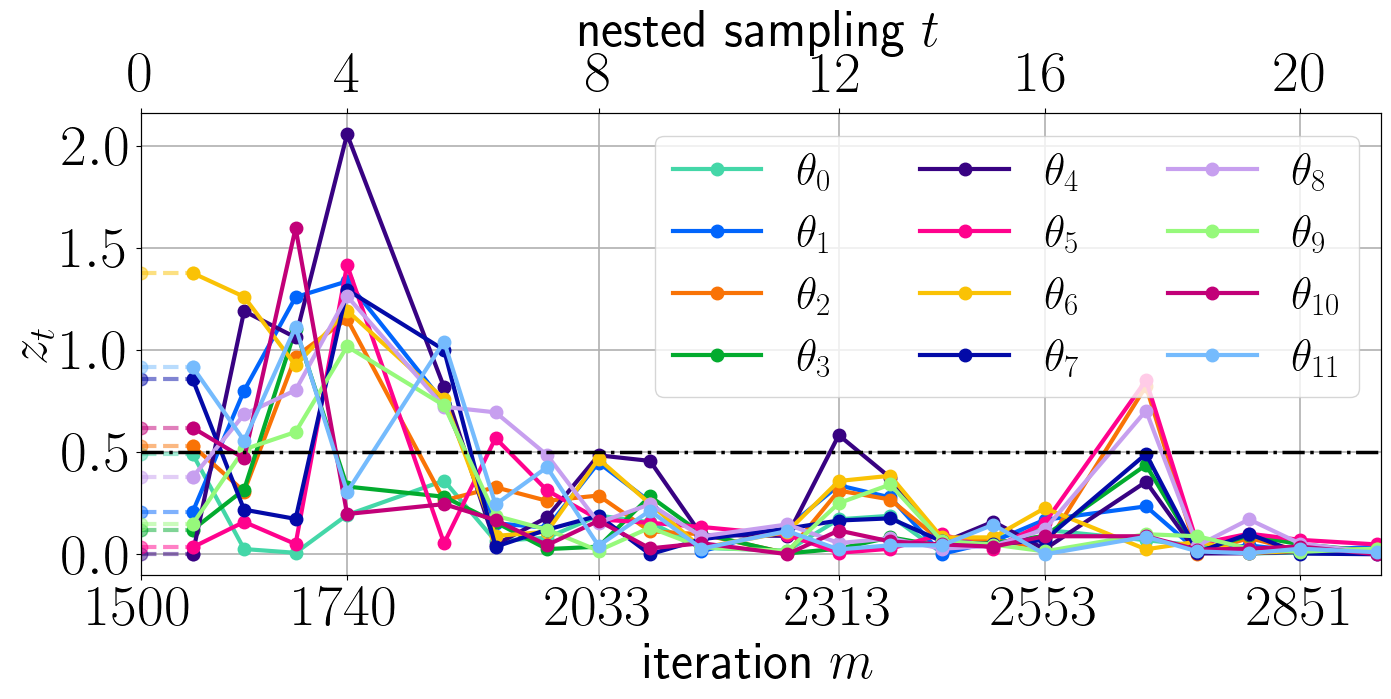
\includegraphics[width=0.8\textwidth]{figs/appendix/convergence/230103_064024_dynesty-sampling_convergence_z_eps0.5.png}
    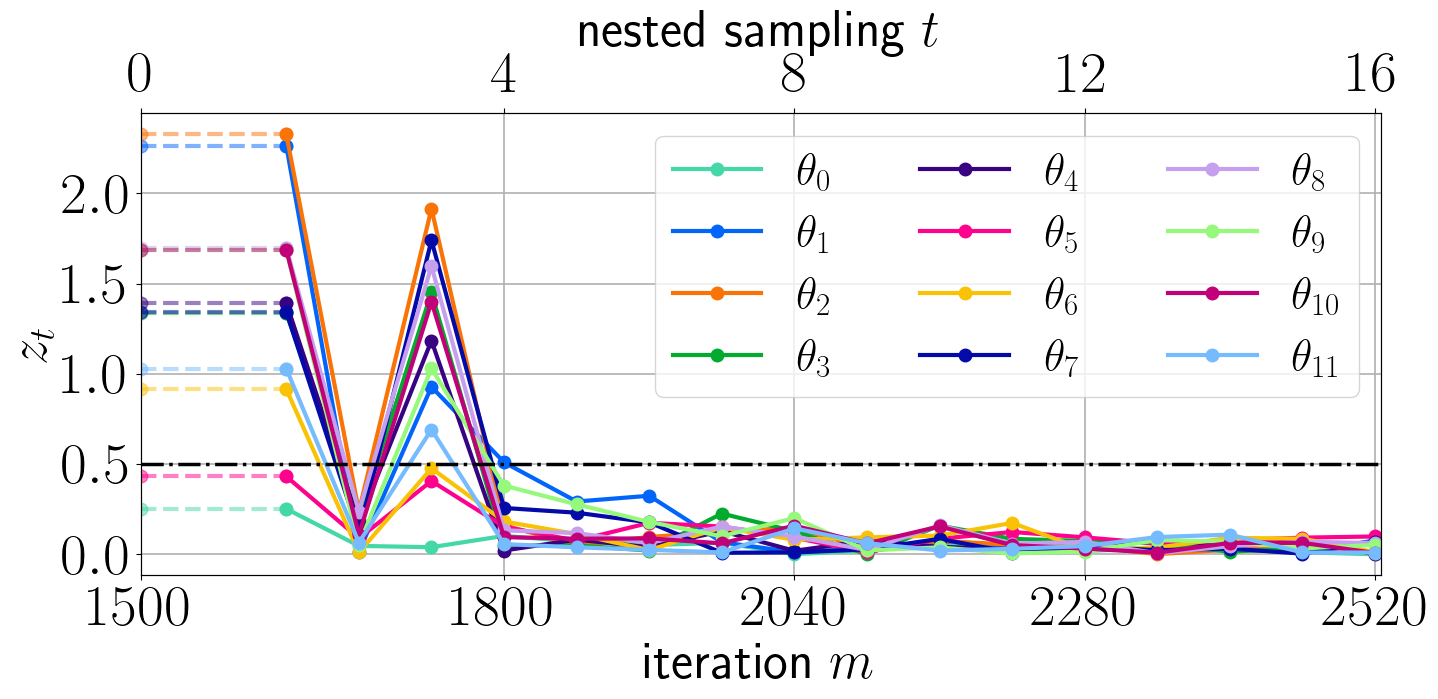
\includegraphics[width=0.8\textwidth]{figs/appendix/convergence/230103_060017_dynesty-sampling_convergence_z_eps0.5.png}
    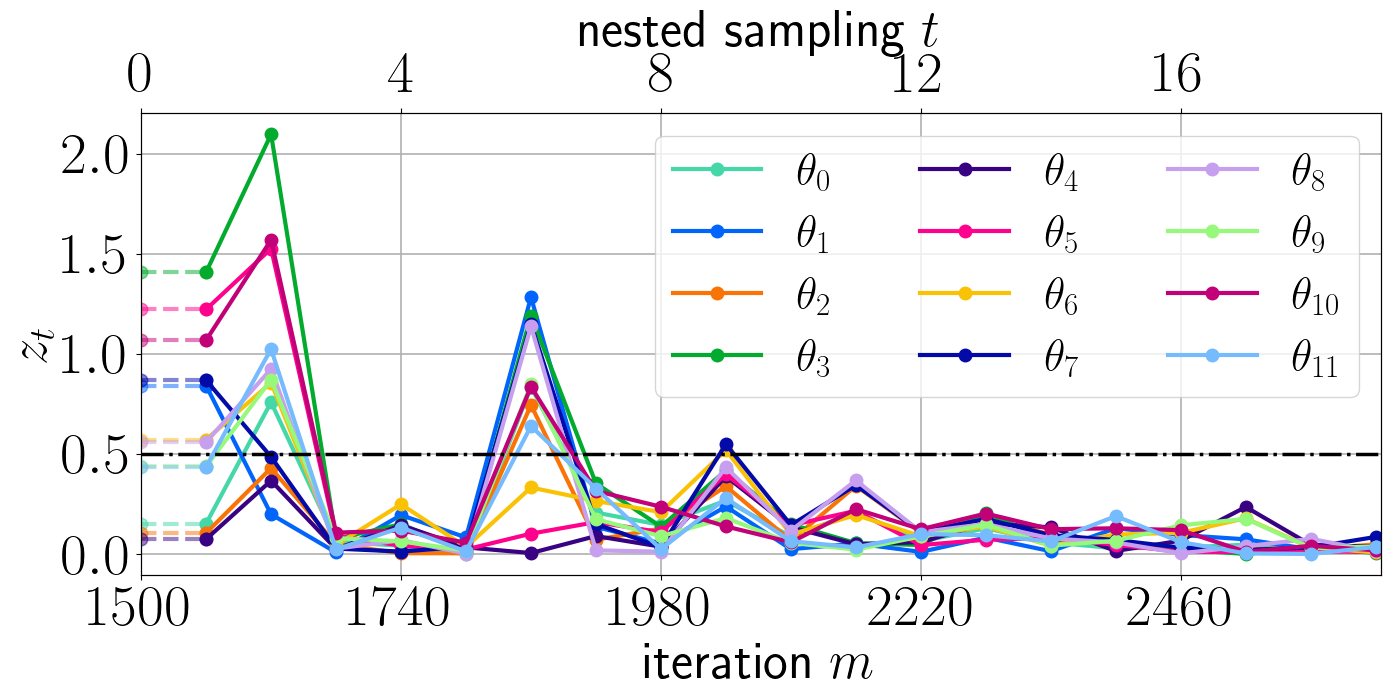
\includegraphics[width=0.8\textwidth]{figs/appendix/convergence/230622_230103_dynesty-sampling_convergence_z_eps0.5.png}
    \figcaption{\textbf{Same as Figure~\ref{fig:convergence_single}, for multi-component equivalents.}}\label{fig:convergence_multi}
\end{figure*}


% ============================

\end{document}
